
% The \appendix command resets the chapter counter, and changes the chapter numbering scheme to capital letters.
%\chapter{Appendices}
\appendix

\clearpage
\phantomsection
\addcontentsline{toc}{chapter}{Appendices}
\addtocontents{toc}{\protect\setcounter{tocdepth}{0}}

\chapter{Dijet Mass Binning}
\label{app:dijet_bins}

\noindent
The dijet mass binning used in the di-$b$-jet analyses, given in units of GeV:
\begin{verbatim}
203, 216, 229, 243, 257, 272, 287, 303, 319, 335, 352, 369,
387, 405, 424, 443, 462, 482, 500, 523, 544, 566, 588, 611, 
634, 657, 681, 705, 730, 755, 781, 807, 834, 861, 889, 917,
946, 976, 1006, 1037, 1068, 1100, 1133, 1166, 1200, 1234, 
1269, 1305, 1341, 1378, 1416, 1454, 1493, 1533, 1573, 1614,
1656, 1698, 1741, 1785, 1830, 1875, 1921, 1968, 2016, 2065, 
2114, 2164, 2215, 2267, 2320, 2374, 2429, 2485, 2542, 2600, 
2659,2719, 2780, 2842, 2905, 2969, 3034, 3100, 3167, 3235, 
3305, 3376, 3448,3521, 3596, 3672, 3749, 3827, 3907, 3988, 
4070, 4154, 4239, 4326, 4414, 4504, 4595, 4688, 4782, 4878, 
4975, 5074, 5175, 5277, 5381, 5487, 5595, 5705, 5817, 5931, 
6047, 6165, 6285, 6407, 6531, 6658, 6787, 6918, 7052, 7188, 
7326, 7467, 7610, 7756, 7904, 8055, 8208, 8364, 8523, 8685, 
8850, 9019, 9191, 9366, 9544, 9726, 9911, 10100, 10292, 
10488, 10688, 10892, 11100, 11312, 11528, 11748, 11972, 
12200, 12432, 12669, 12910, 13156
\end{verbatim}


\chapter{Single Jet Trigger Threshold~\pT{} Fit}
\label{app:triggerTurnOn_fit}

The trigger plateau is defined as the kinematic region where all events that pass the offline jet-\pT{} selection
also pass the online jet-\pT{} selection at the trigger level.
To be on the trigger plateau of a single jet trigger
the offline jet-\pT{} must be above some threshold value,
which is referred to as the threshold jet-\pT{}.

For single jet triggers it is found that the threshold offline jet-\pT{} follows
a linear behaviour with respect to the online jet-\pT{} requirements at the trigger level.
Therefore a linear fit can be used to predict the threshold jet-\pT{} of any single jet trigger
from considering a small number of single jet triggers.
The single jet triggers considered require that there is an online jet with \pT{} above
15, 25, 35, 45, 60, 110, 175, 260 and 360 GeV respectively.
%are \verb|HLT_j15|, \verb|HLT_j25|, \verb|HLT_j35|, \verb|HLT_j45|,
%\verb|HLT_j60|, \verb|HLT_j110| , \verb|HLT_j175| , \verb|HLT_j260| and \verb|HLT_j360|,
%where, as an example, \verb|HLT_j360| requires that there is an online jet with \pT{}~\gt{}~360~GeV.

Figure~\ref{fig:triggerTurnOn_fit} shows the threshold jet-\pT{} 
at which a trigger is 99\% efficient with respect to a lower-\pT{} benchmark trigger
as a function of the jet-\pT{} requirement of the single jet trigger.
A linear fit is performed, as shown by the red line.
The 1$\sigma$ error band on the fit slope is shown by the dotted lines~\cite{evt-jet_turnOnFit}.

\begin{figure}[!hbt]
    \begin{center}
        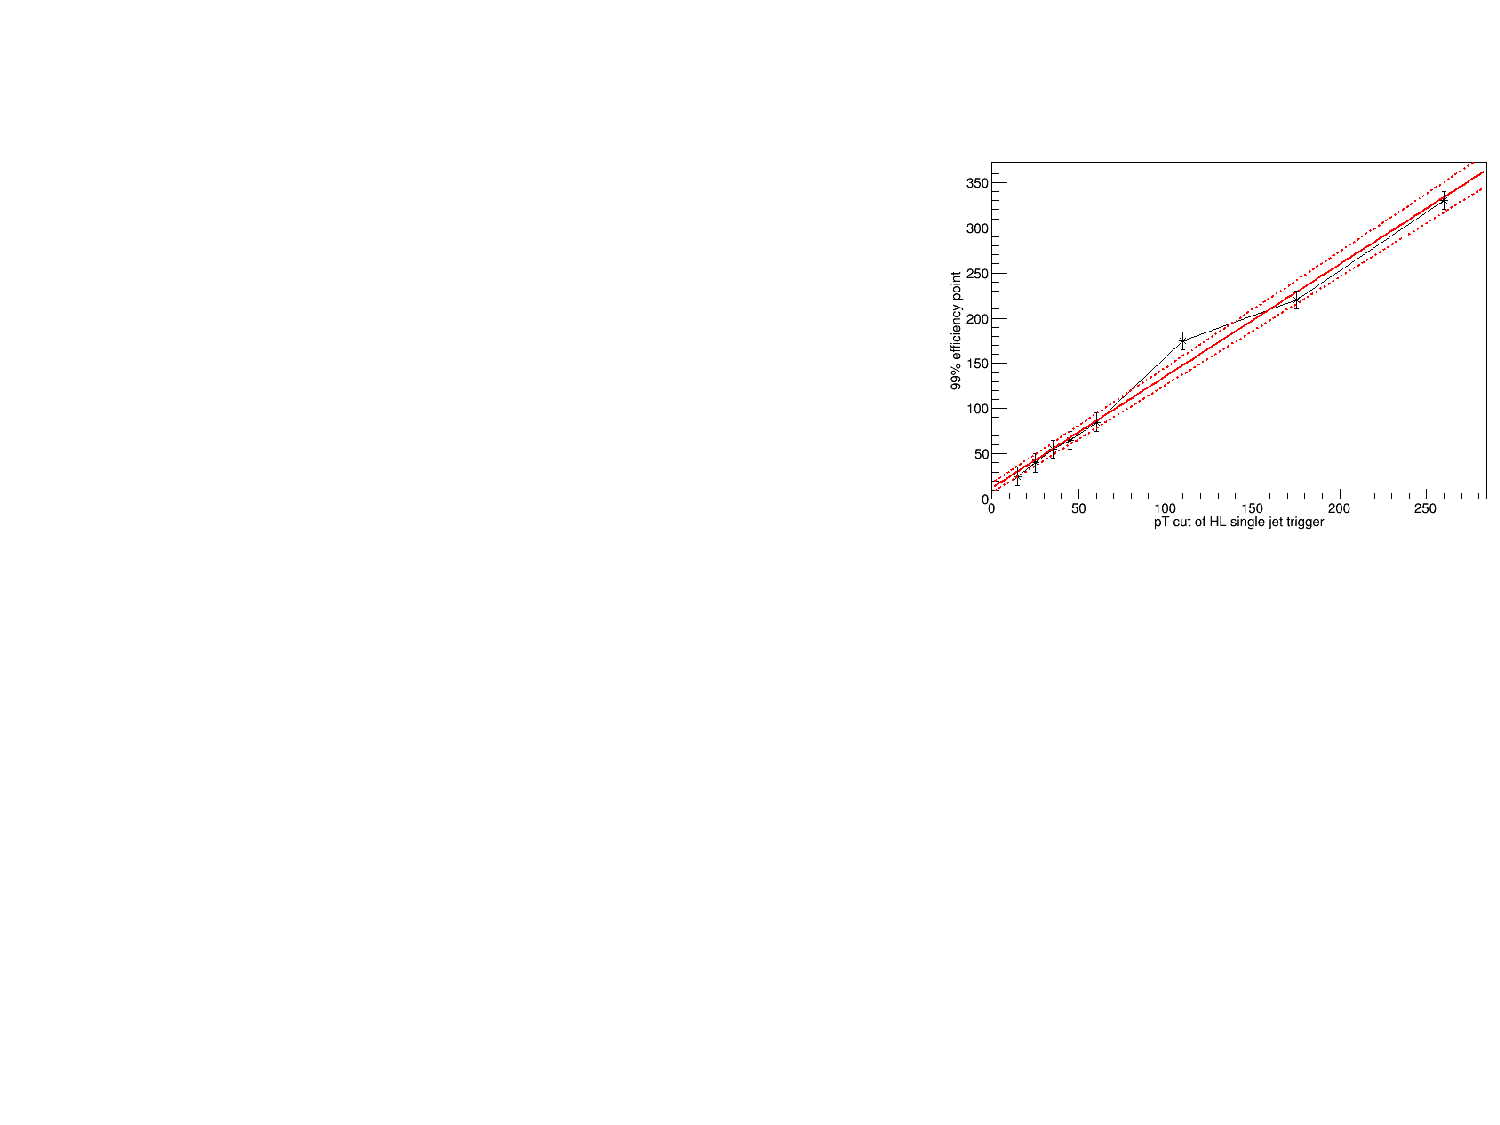
\includegraphics[width=0.7\linewidth, angle=0]{figs/Dibjet/LowMass/jetTriggerTurnOn.pdf}
      \end{center}
  \caption[A plot showing the threshold jet-\pT{} of a single jet trigger as a function of the trigger-level jet-\pT{} requirements.]
           {A plot showing the threshold offline jet-\pT{} at which a trigger is 99\% efficient
             with respect to a lower-\pT{} benchmark trigger as a function of the trigger-level~\pT{} requirements of the single jet trigger.
             A linear fit is performed, as shown by the red line. The 1$\sigma$ error band on the fit slope is shown by the dotted lines~\cite{evt-jet_turnOnFit}.}
          \label{fig:triggerTurnOn_fit}
\end{figure}

\noindent
The resulting linear fit has a normalisation of 12.3 and a slope of 1.24.
Applying the fit to the trigger level jet requirements of the double $b$-jet trigger we obtain:
\vspace{-0.5em}
\begin{itemize}[leftmargin=*]
\item Trigger level jet~\pT{} $>$ 150 GeV,~  Threshold offline jet~\pT{} $>$ 198~GeV 
\item Trigger level jet~\pT{} $>$  50 GeV,~~ Threshold offline jet~\pT{} $>$ 74.1~GeV
\end{itemize}
\vspace{-0.3em}
\noindent
The values are rounded up in the analysis to give a safety margin.

%\chapter{All SWiFt Configurations for \lm{} Data-Set Fit Validation Studies}
\chapter{Additional Plots for \lm{} Data-Set Fit Validation Studies}
\label{app:lowMass_Swift}
\vspace{-3em}

\section{Figure~\ref{fig:bumpH_spuriousSignal} for all SWiFt configurations}

\begin{figure}[!htb]
\captionsetup[subfigure]{aboveskip=0pt,justification=centering}
\centering
\subcaptionbox{4 parameter fit, $wHW$ = 16} {
  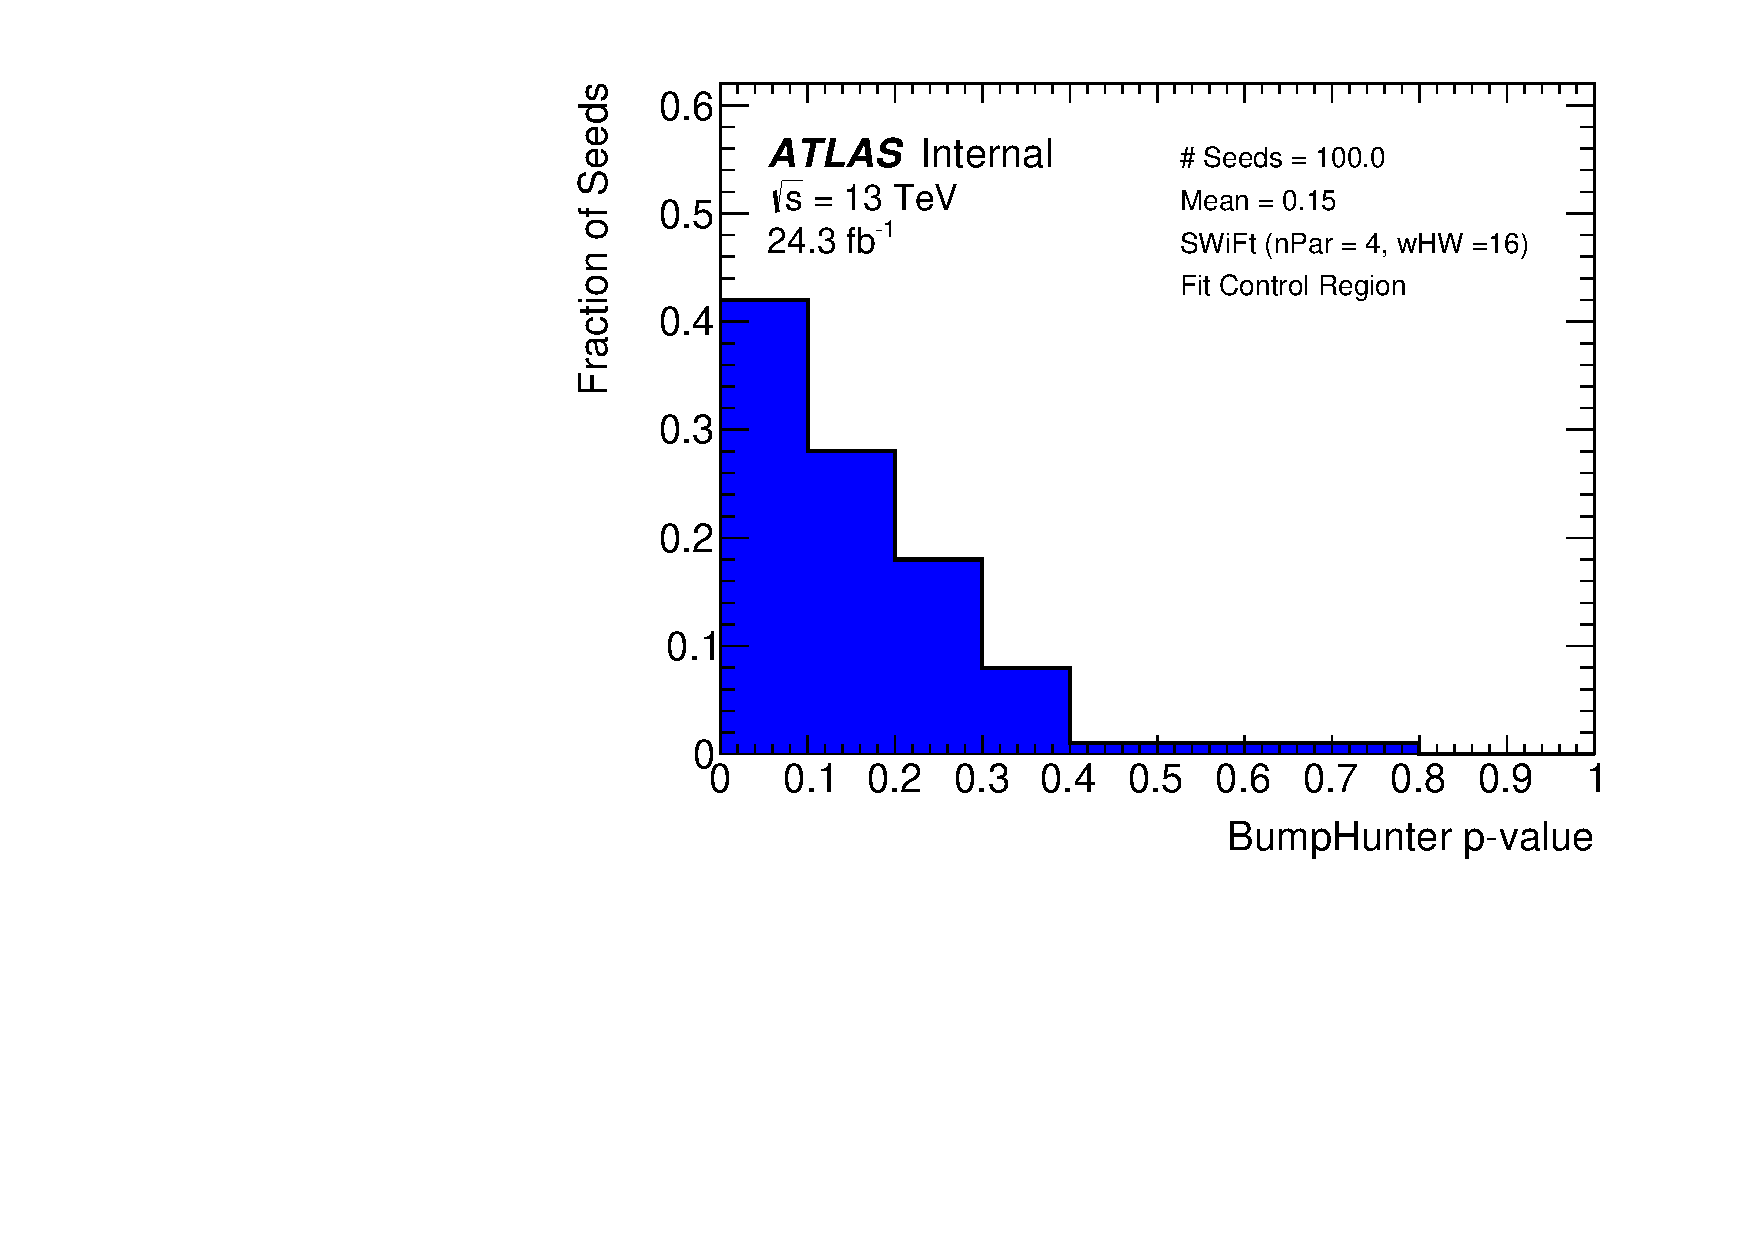
\includegraphics[width=0.48\linewidth, angle=0]{figs/Dibjet/LowMass/FitStudy_min566/pVal_bumpHunter_corrFitCR_4para_low16_high16.pdf}
}\hspace{-3mm}                                       
\subcaptionbox{4 parameter fit, $wHW$ = 14} {                                                    
  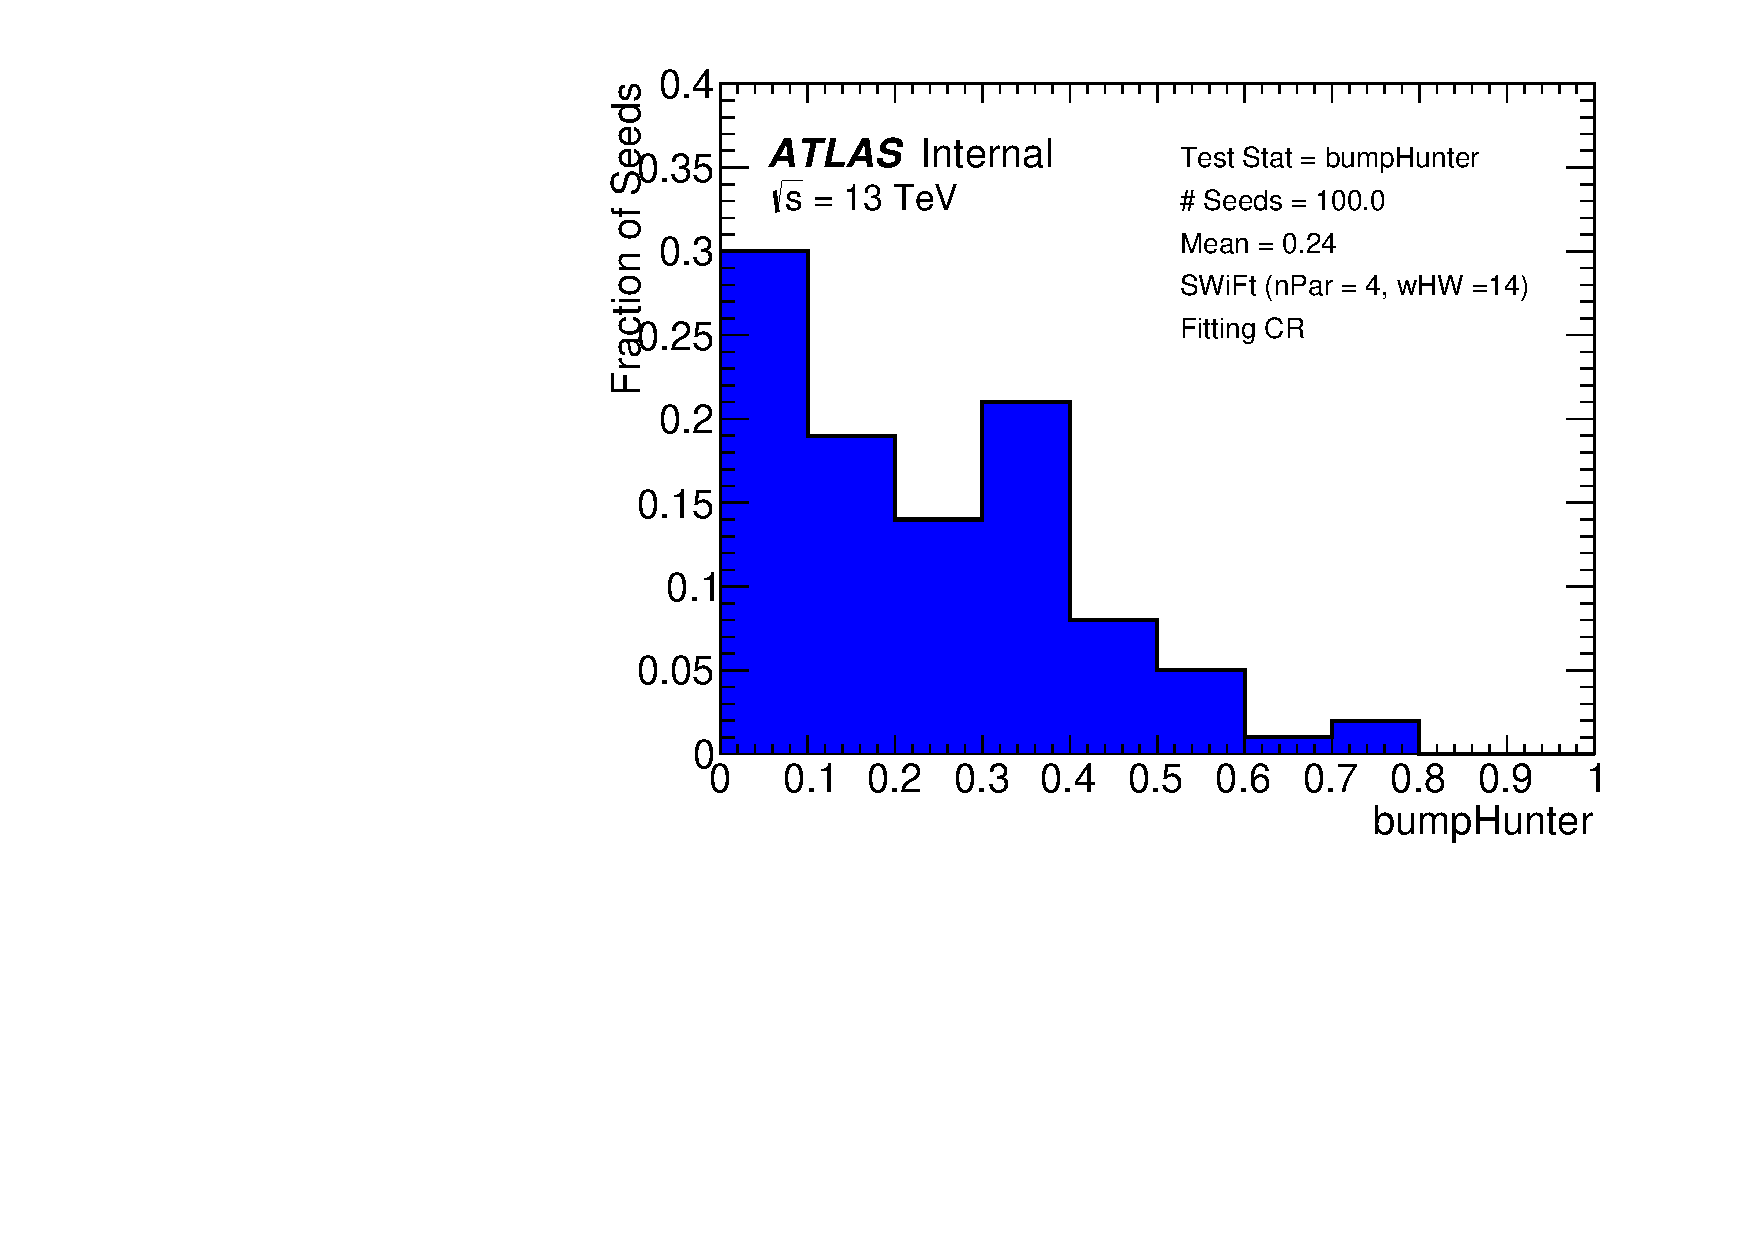
\includegraphics[width=0.48\linewidth, angle=0]{figs/Dibjet/LowMass/FitStudy_min566/pVal_bumpHunter_corrFitCR_4para_low14_high14.pdf}
}\hspace{-3mm}                                       
\subcaptionbox{4 parameter fit, $wHW$ = 12} {                                                    
  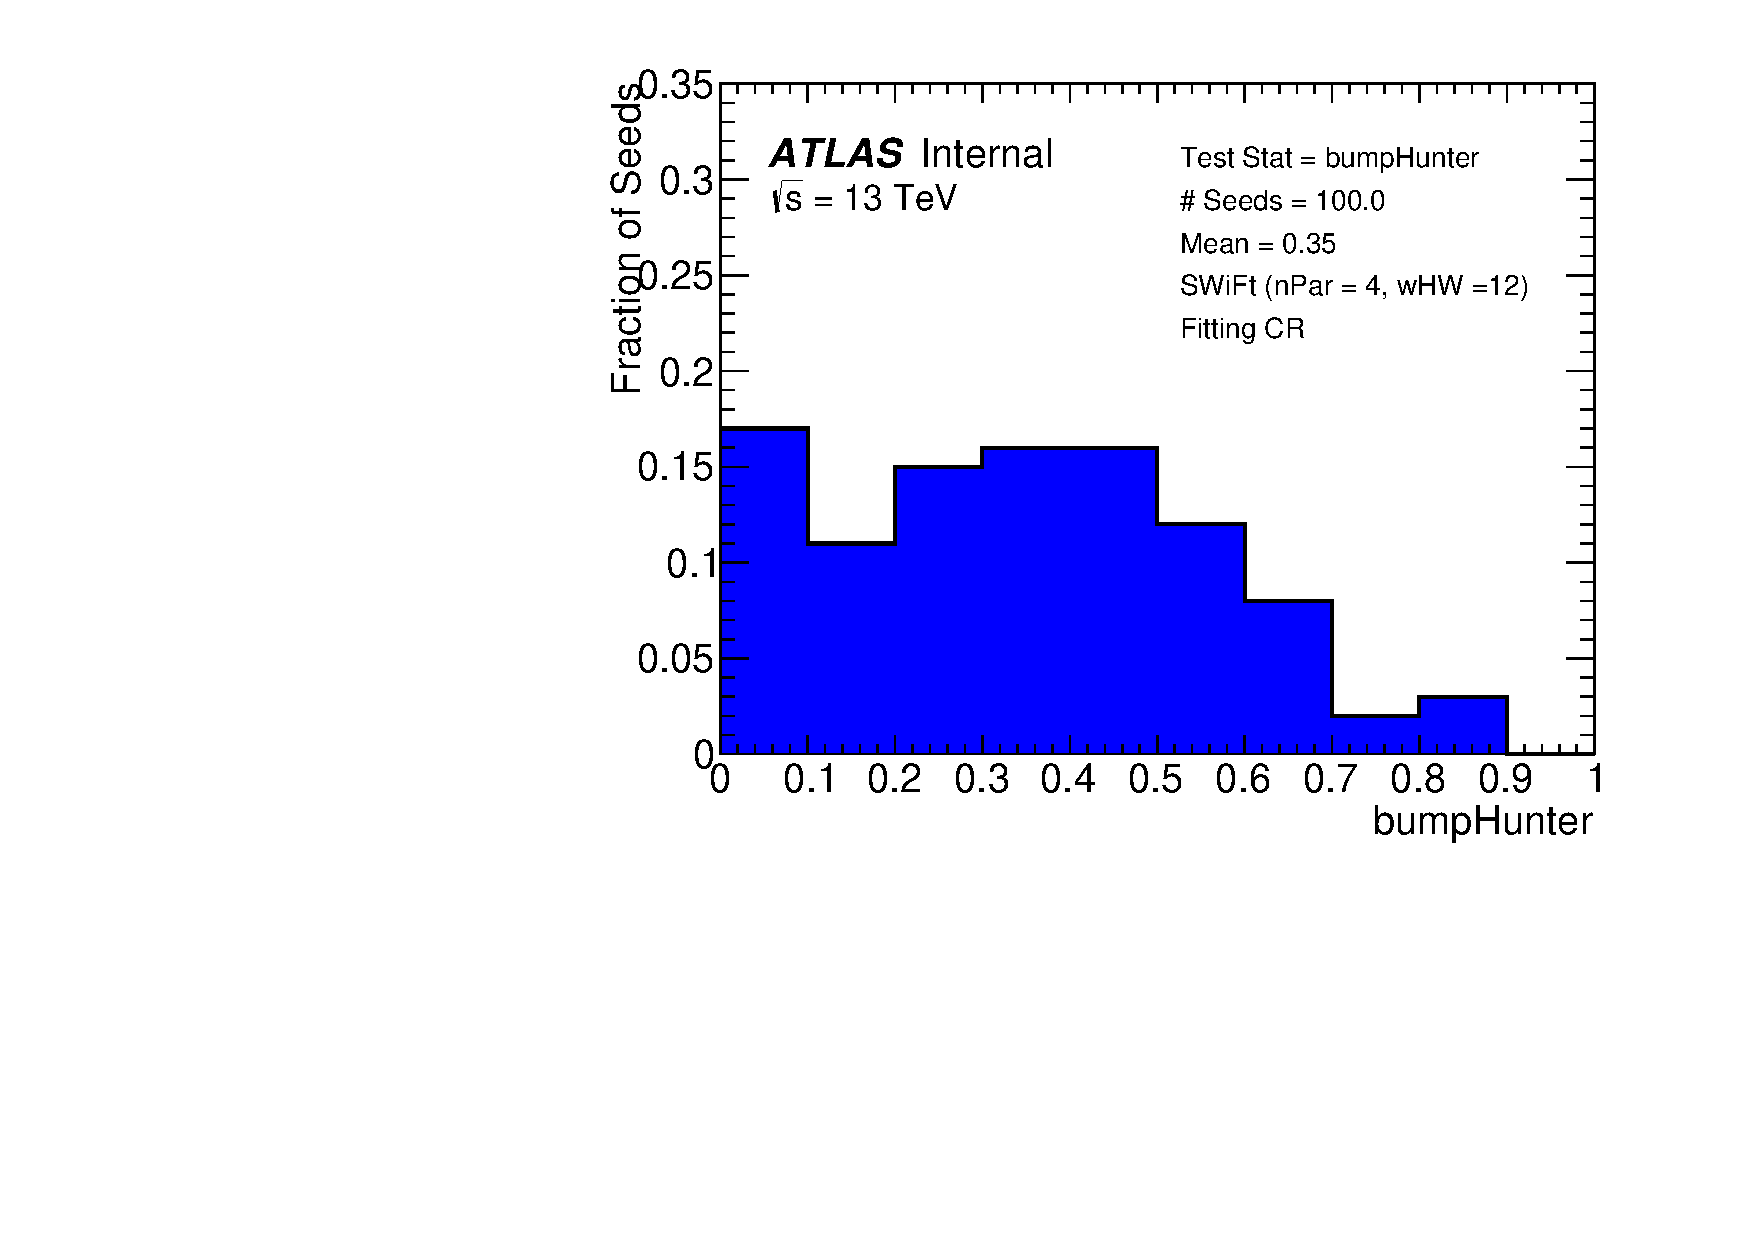
\includegraphics[width=0.48\linewidth, angle=0]{figs/Dibjet/LowMass/FitStudy_min566/pVal_bumpHunter_corrFitCR_4para_low12_high12.pdf}
}\hspace{-3mm}                                       
\subcaptionbox{4 parameter fit, $wHW$ = 10} {                                                    
  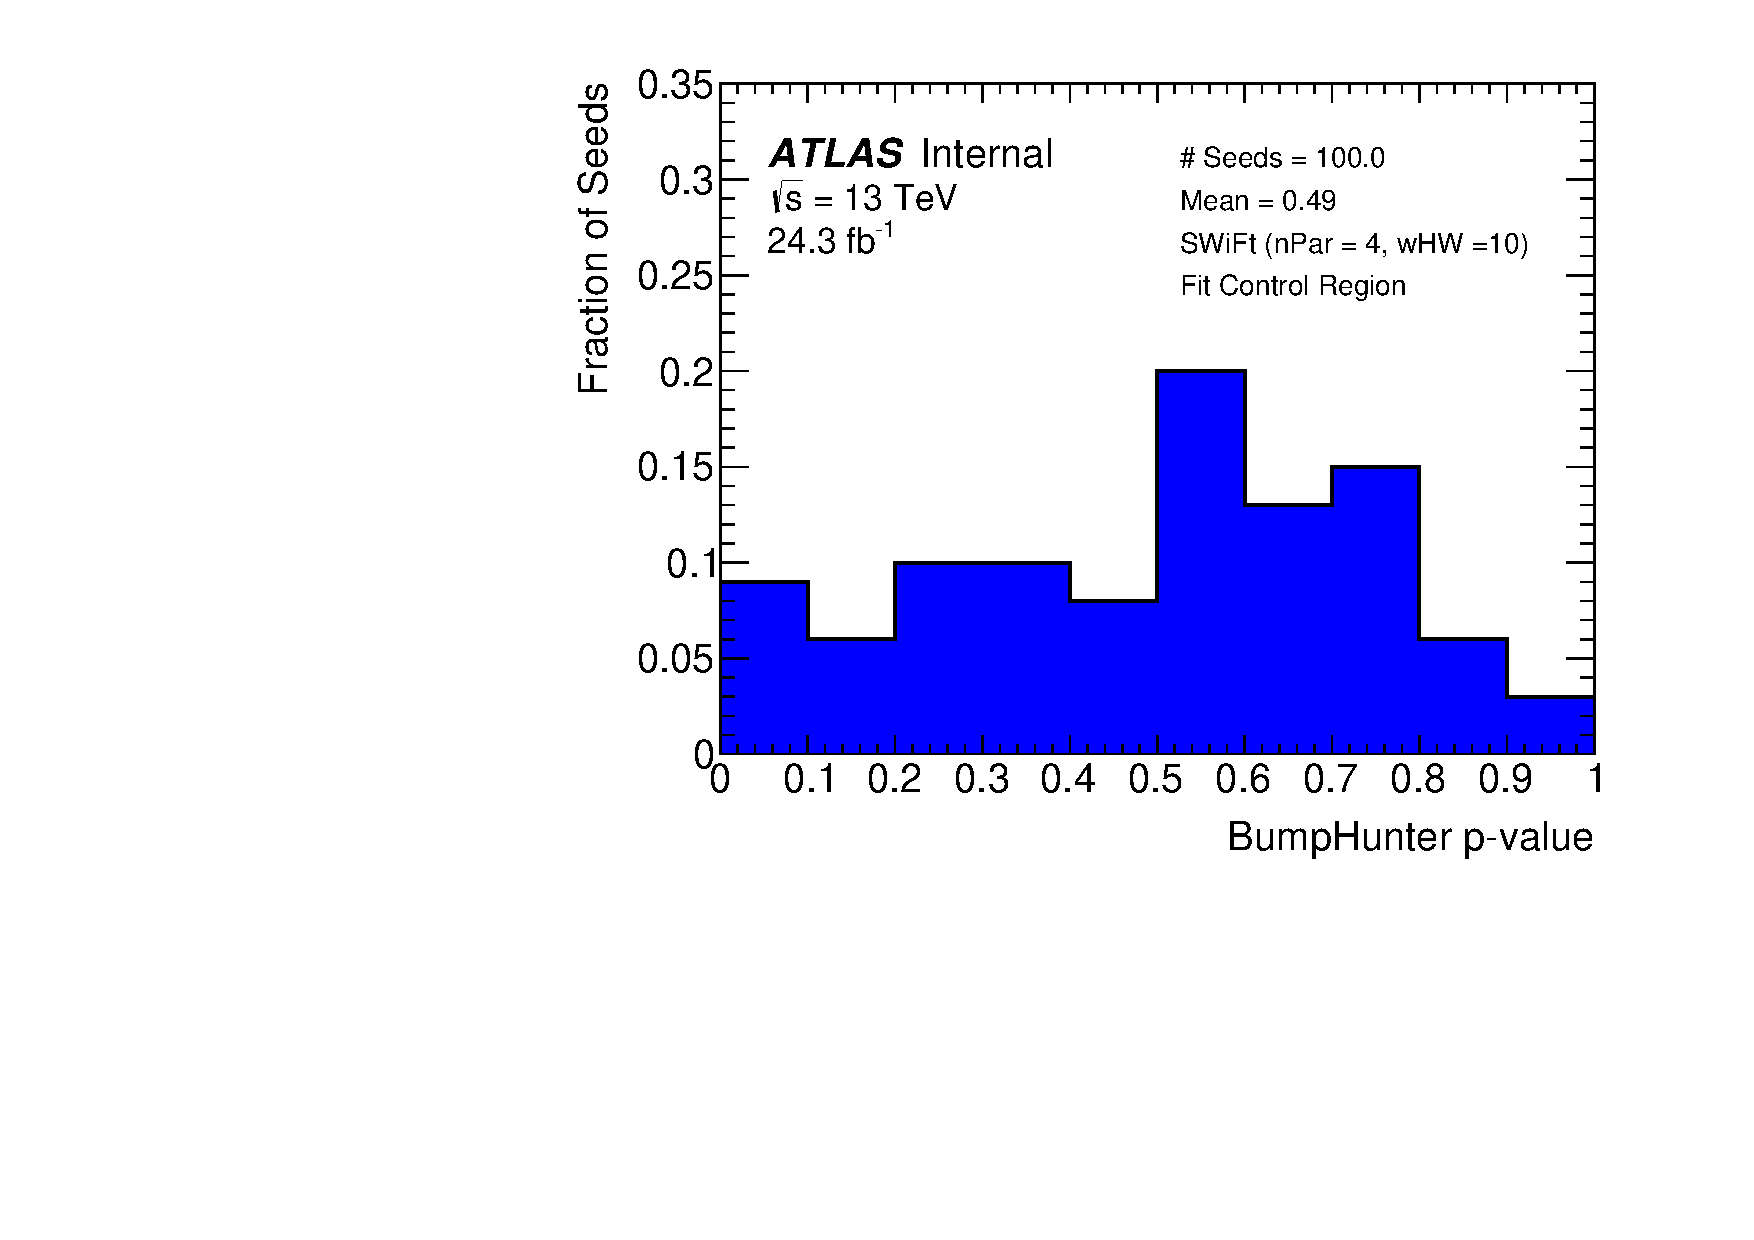
\includegraphics[width=0.48\linewidth, angle=0]{figs/Dibjet/LowMass/FitStudy_min566/pVal_bumpHunter_corrFitCR_4para_low10_high10.pdf}
}\hspace{-3mm}
\caption[Figure~\ref{fig:bumpH_spuriousSignal} for all SWiFt configurations using the 4 parameter dijet fit function.]
 {\label{fig:app-bumpH_spuriousSignal_4para}
 Figure~\ref{fig:bumpH_spuriousSignal} for all SWiFt configurations using the 4 parameter dijet fit function.
  This figure shows the normalised distribution of \bh{} $p$-values from performing the SWiFt background estimate to an ensemble of
  data-like dijet mass spectra taken from the fit control region for the \lm{} data-set.
  The SWiFt configurations considered use the 4 parameter dijet fit function for a window half-width ($wHW$) range of 10 to 16.
}
\end{figure}

\begin{figure}[!htb]
\captionsetup[subfigure]{aboveskip=0pt,justification=centering}
\subcaptionbox{5 parameter fit, $wHW$ = 16} {                                                    
  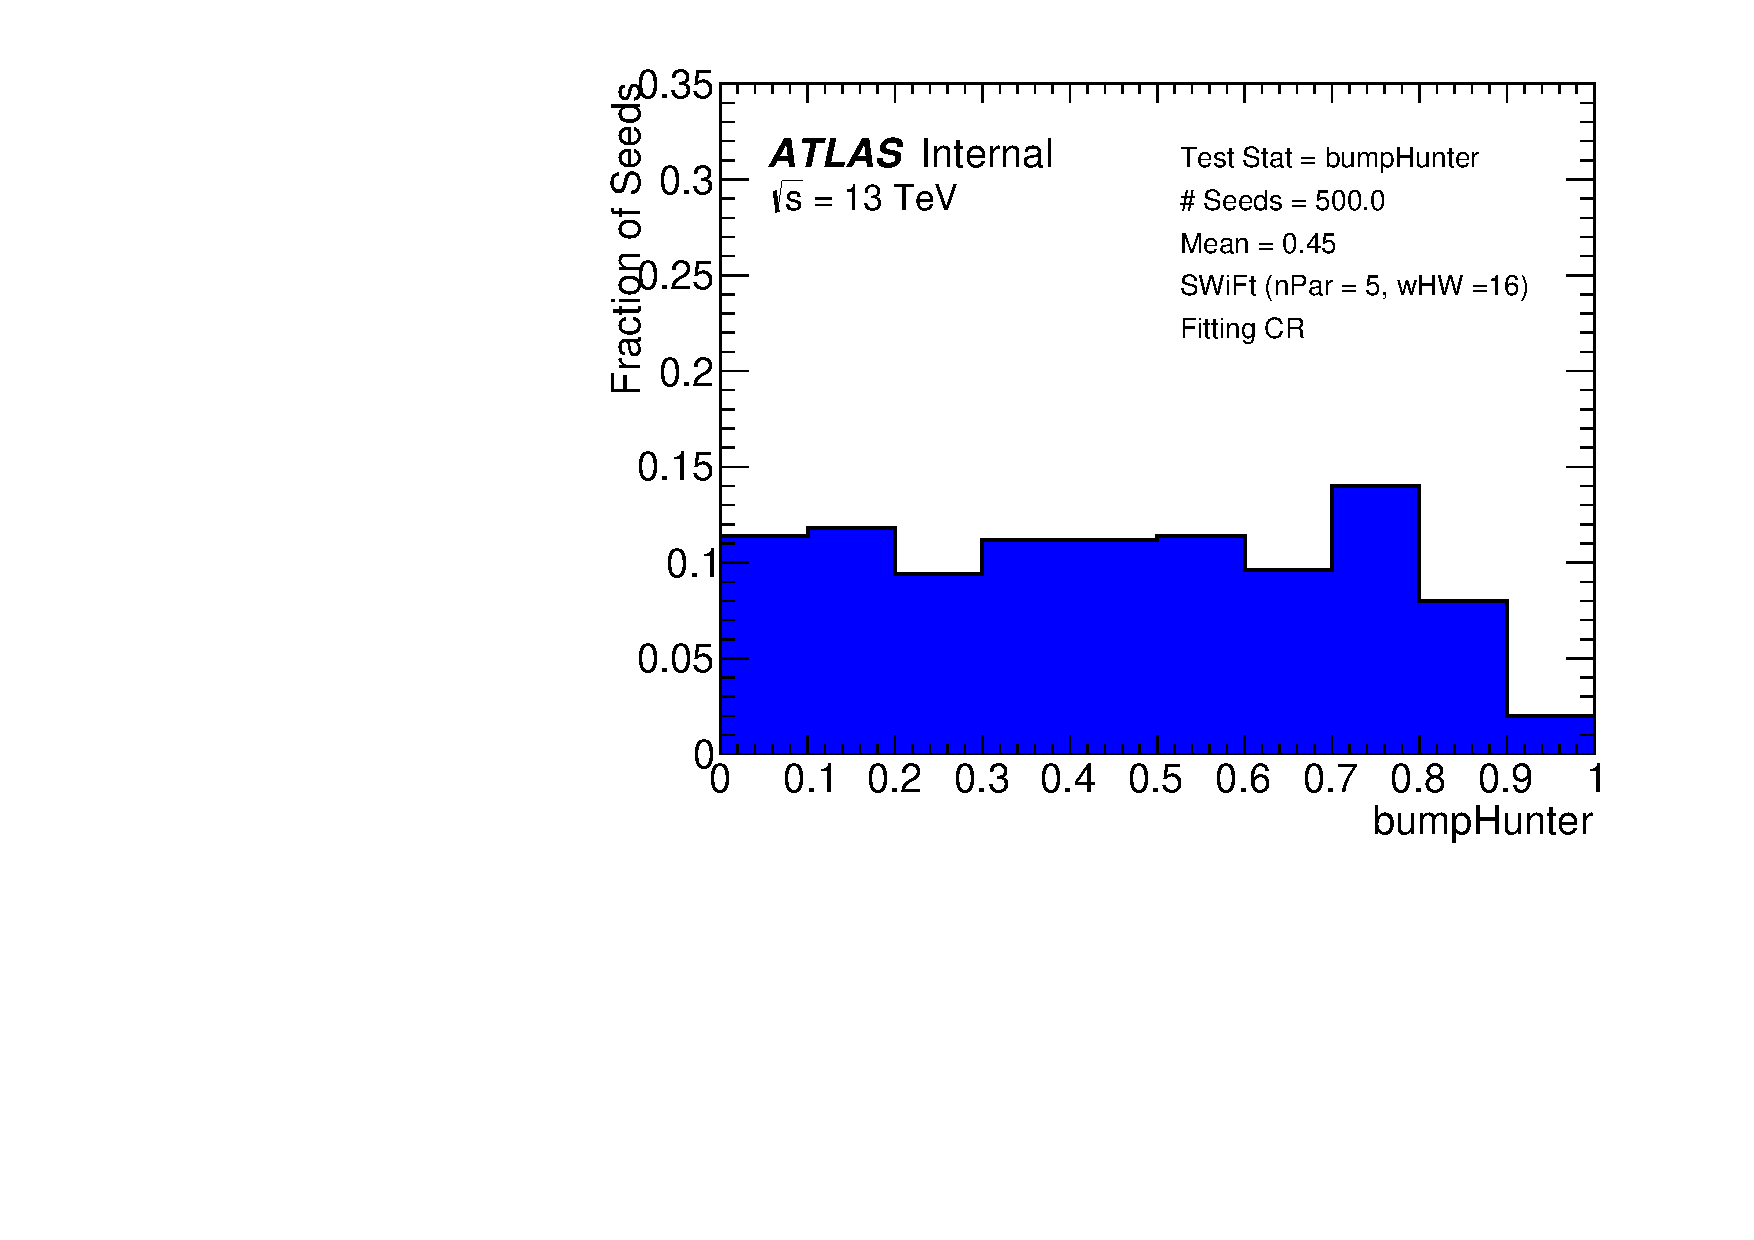
\includegraphics[width=0.48\linewidth, angle=0]{figs/Dibjet/LowMass/FitStudy_min566/pVal_bumpHunter_corrFitCR_5para_low16_high16.pdf}
}\hspace{-3mm}                                       
\subcaptionbox{5 parameter fit, $wHW$ = 14} {                                                    
  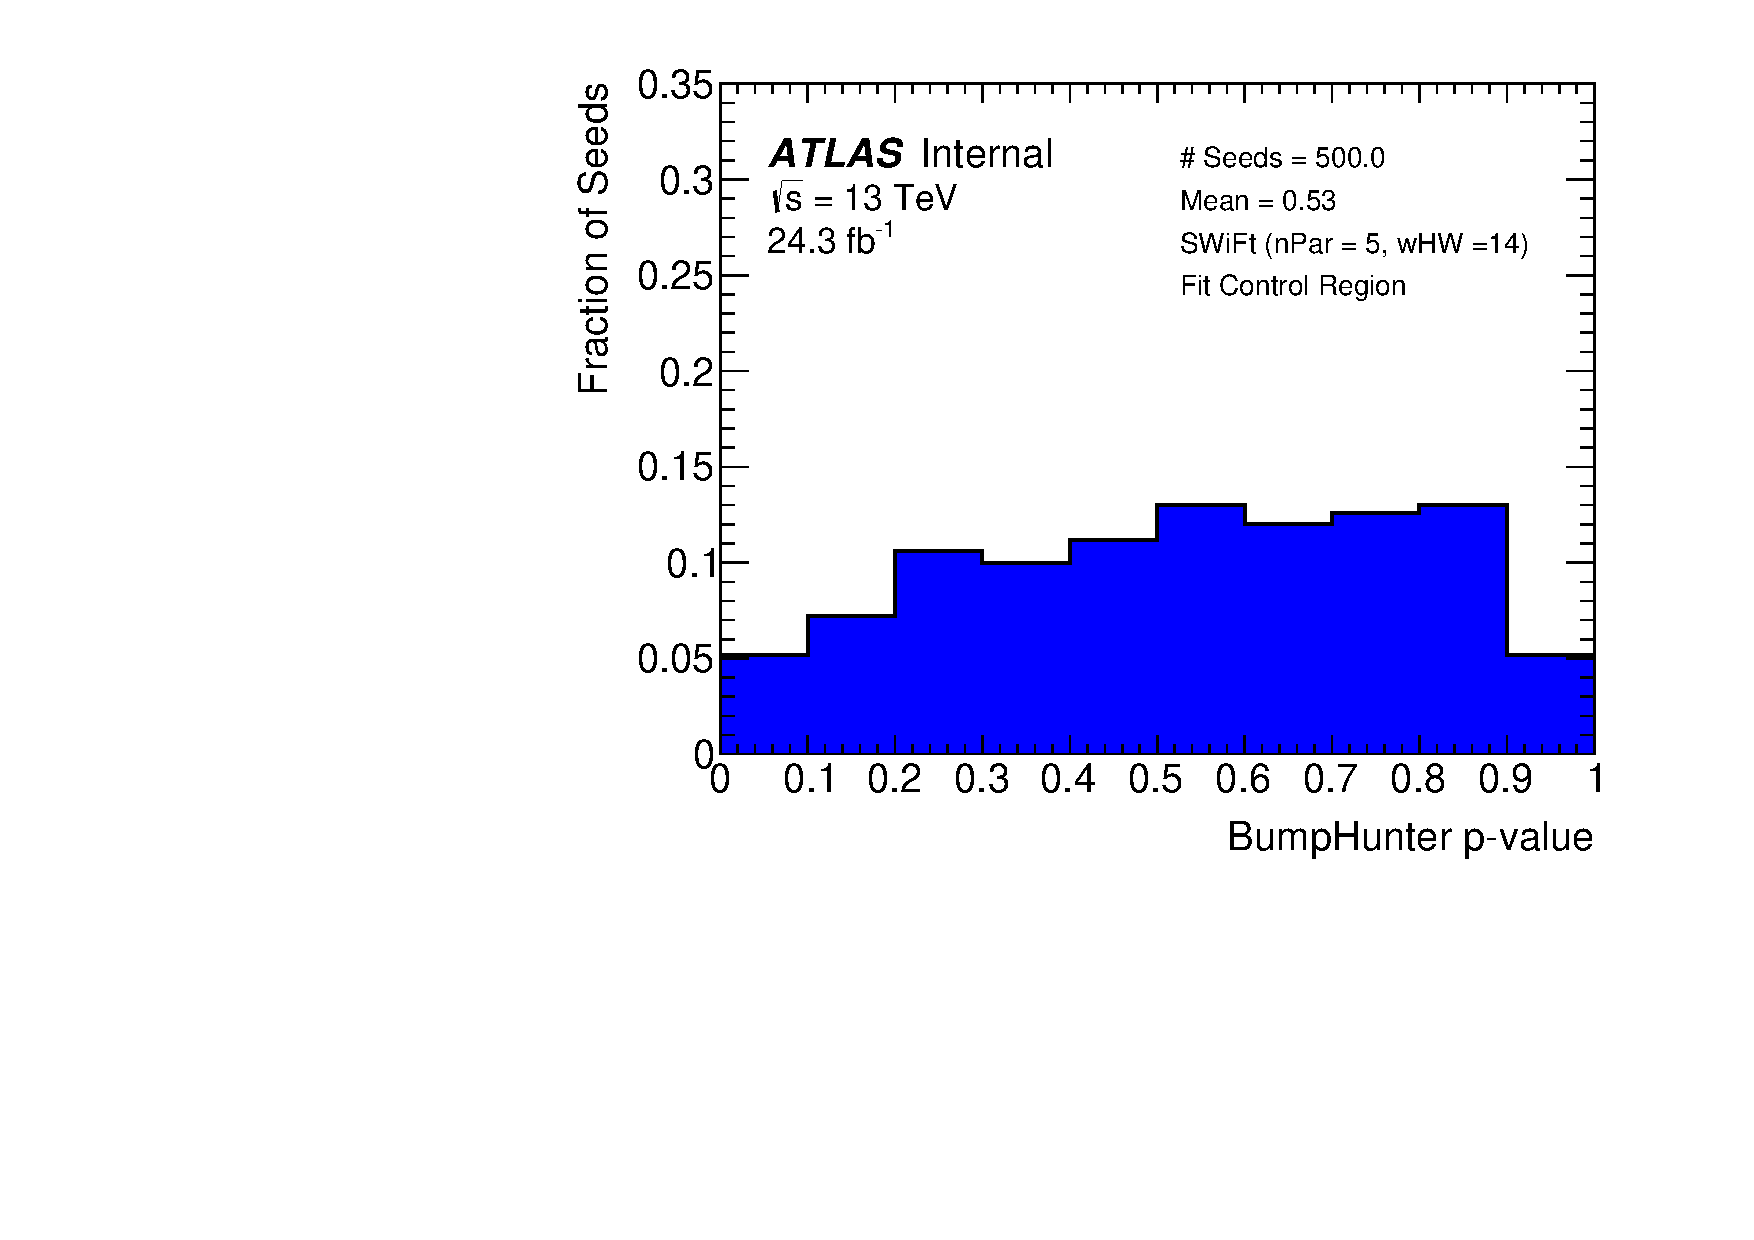
\includegraphics[width=0.48\linewidth, angle=0]{figs/Dibjet/LowMass/FitStudy_min566/pVal_bumpHunter_corrFitCR_5para_low14_high14.pdf}
}\hspace{-3mm}                                       
\subcaptionbox{5 parameter fit, $wHW$ = 12} {                                                    
  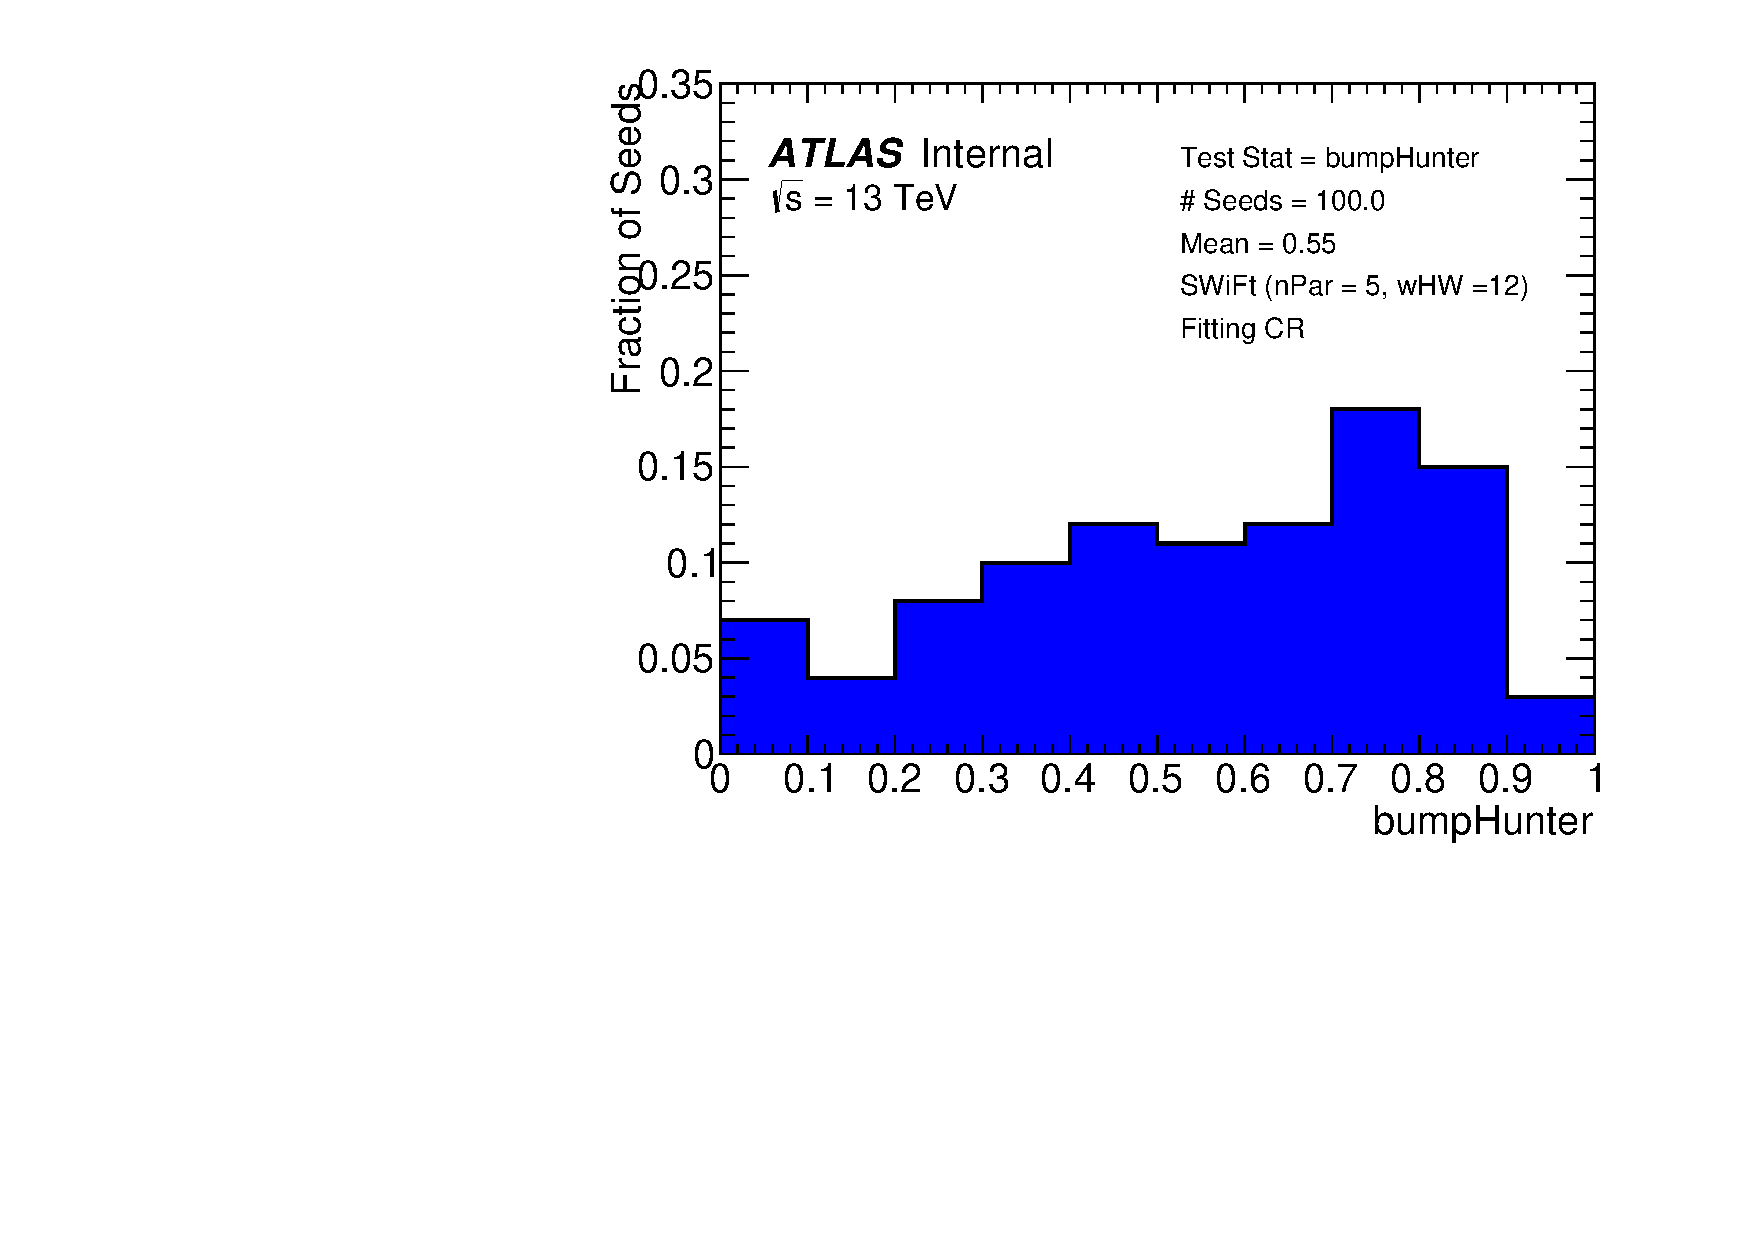
\includegraphics[width=0.48\linewidth, angle=0]{figs/Dibjet/LowMass/FitStudy_min566/pVal_bumpHunter_corrFitCR_5para_low12_high12.pdf}
}\hspace{-3mm}                                       
\subcaptionbox{5 parameter fit, $wHW$ = 10} {                                                    
  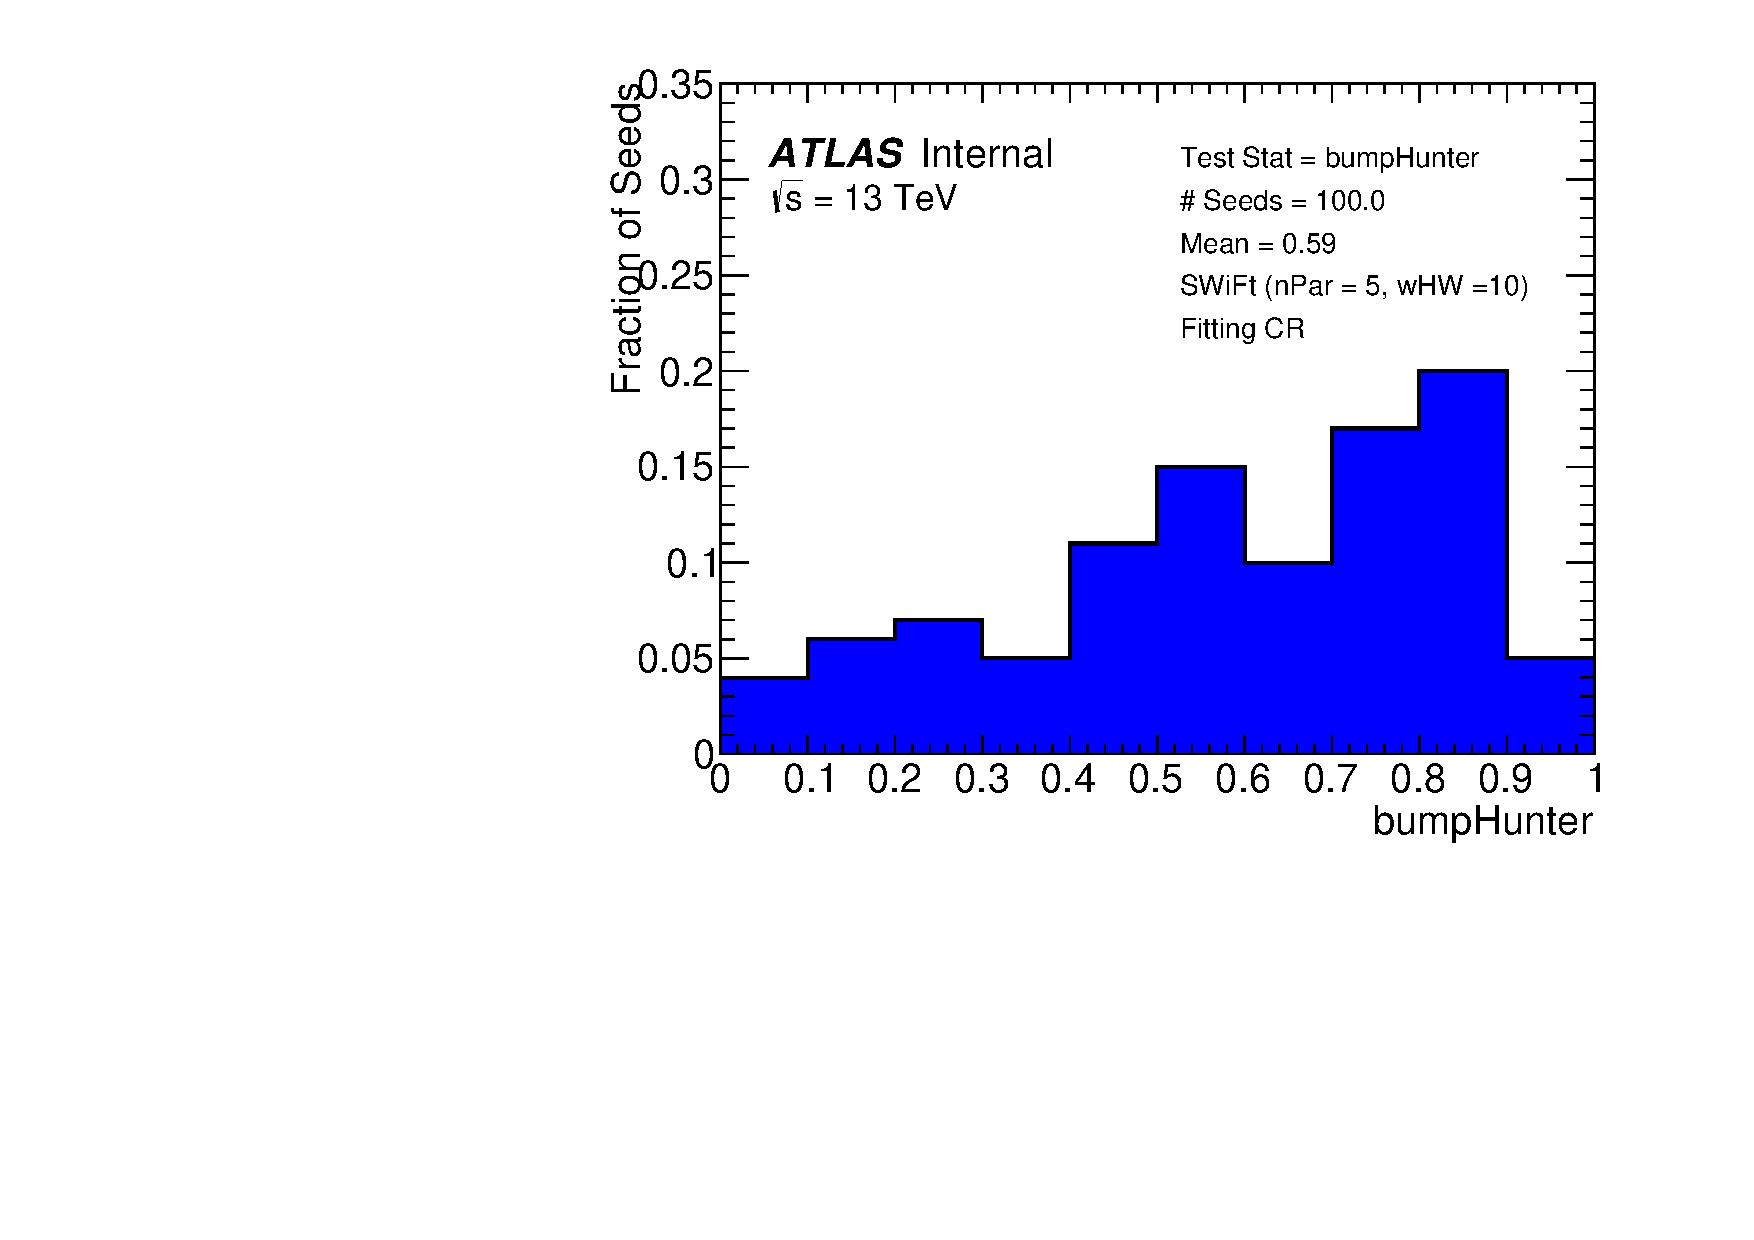
\includegraphics[width=0.48\linewidth, angle=0]{figs/Dibjet/LowMass/FitStudy_min566/pVal_bumpHunter_corrFitCR_5para_low10_high10.pdf}
}
\caption[Figure~\ref{fig:bumpH_spuriousSignal} for all SWiFt configurations using the 5 parameter dijet fit function.]
 {\label{fig:app-bumpH_spuriousSignal_5para}
 Figure~\ref{fig:bumpH_spuriousSignal} for all SWiFt configurations using the 5 parameter dijet fit function..
  This figure shows the normalised distribution of \bh{} $p$-values from performing the SWiFt background estimate to an ensemble of
  data-like dijet mass spectra taken from the fit control region for the \lm{} data-set.
  The SWiFt configurations considered use the 5 parameter dijet fit function for a window half-width ($wHW$) range of 10 to 16.
}
\end{figure}

\clearpage

\section{Figure~\ref{fig:bhFit_lm_corrFitCR_smooth} for all SWiFt configurations}
\vspace{5em}


\begin{figure}[!htb]
\captionsetup[subfigure]{aboveskip=0pt,justification=centering}
\centering
\subcaptionbox{4 parameter fit, $wHW$ = 16} {
  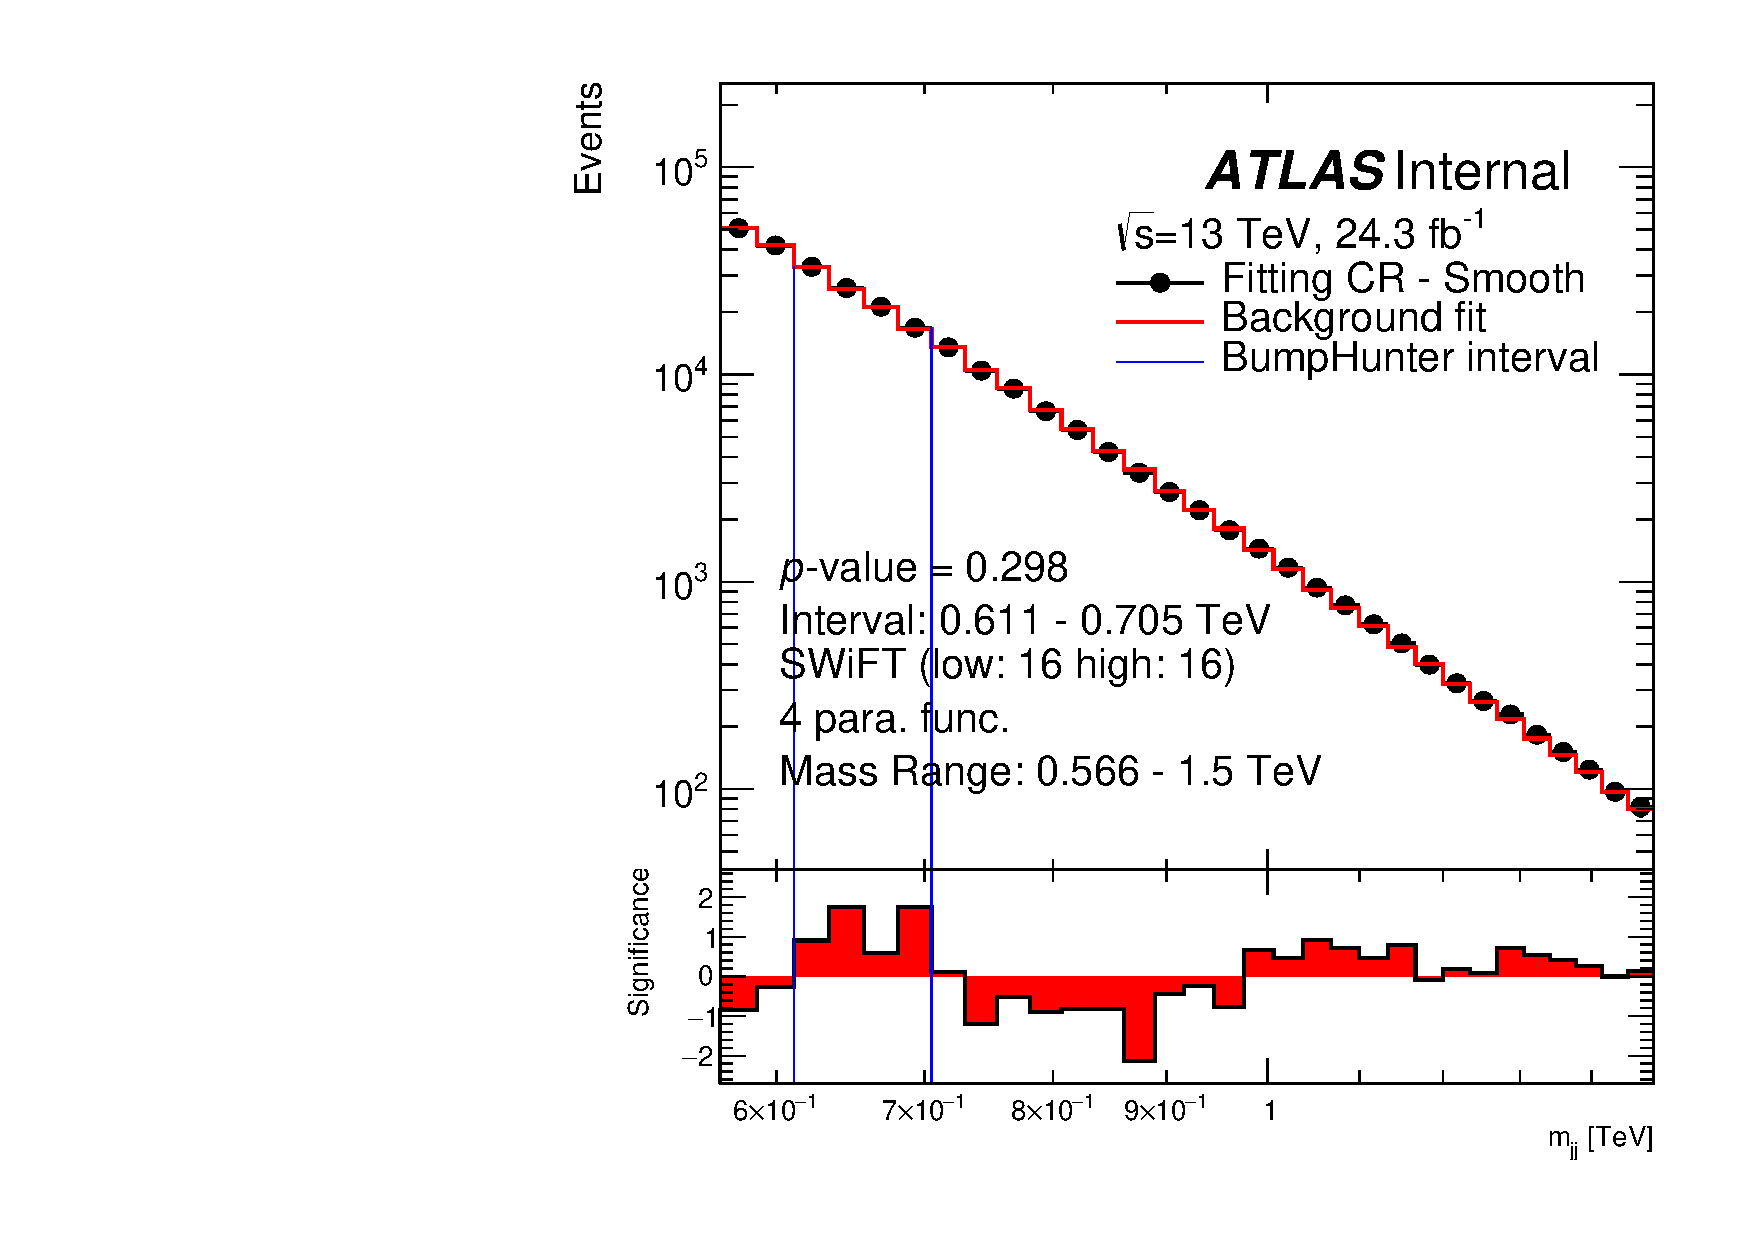
\includegraphics[width=0.48\linewidth, angle=0]{figs/Dibjet/LowMass/FitStudy_min566/bhFit_corrFitCR_smooth_4para_low16_high16.pdf}
}
\subcaptionbox{4 parameter fit, $wHW$ = 14} {
  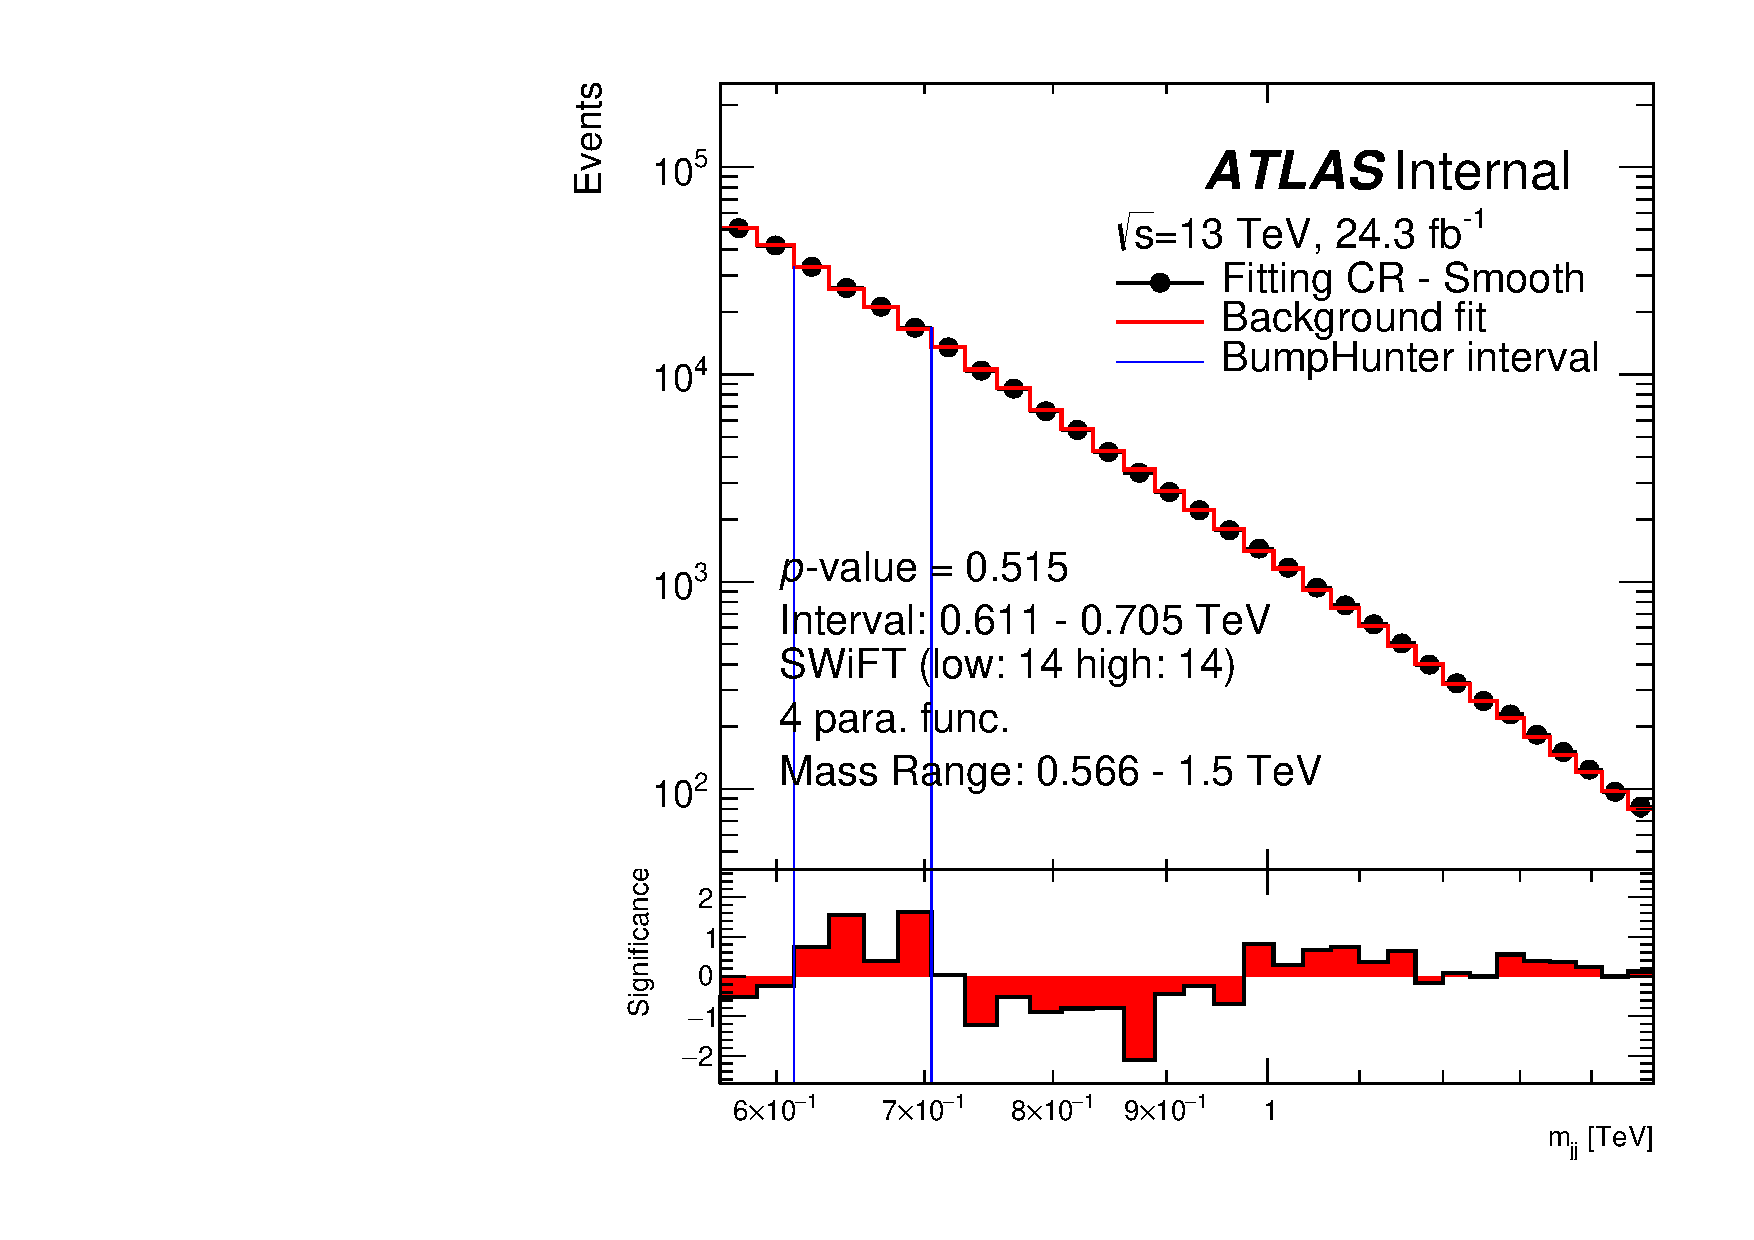
\includegraphics[width=0.48\linewidth, angle=0]{figs/Dibjet/LowMass/FitStudy_min566/bhFit_corrFitCR_smooth_4para_low14_high14.pdf}
}
\subcaptionbox{4 parameter fit, $wHW$ = 12} {
  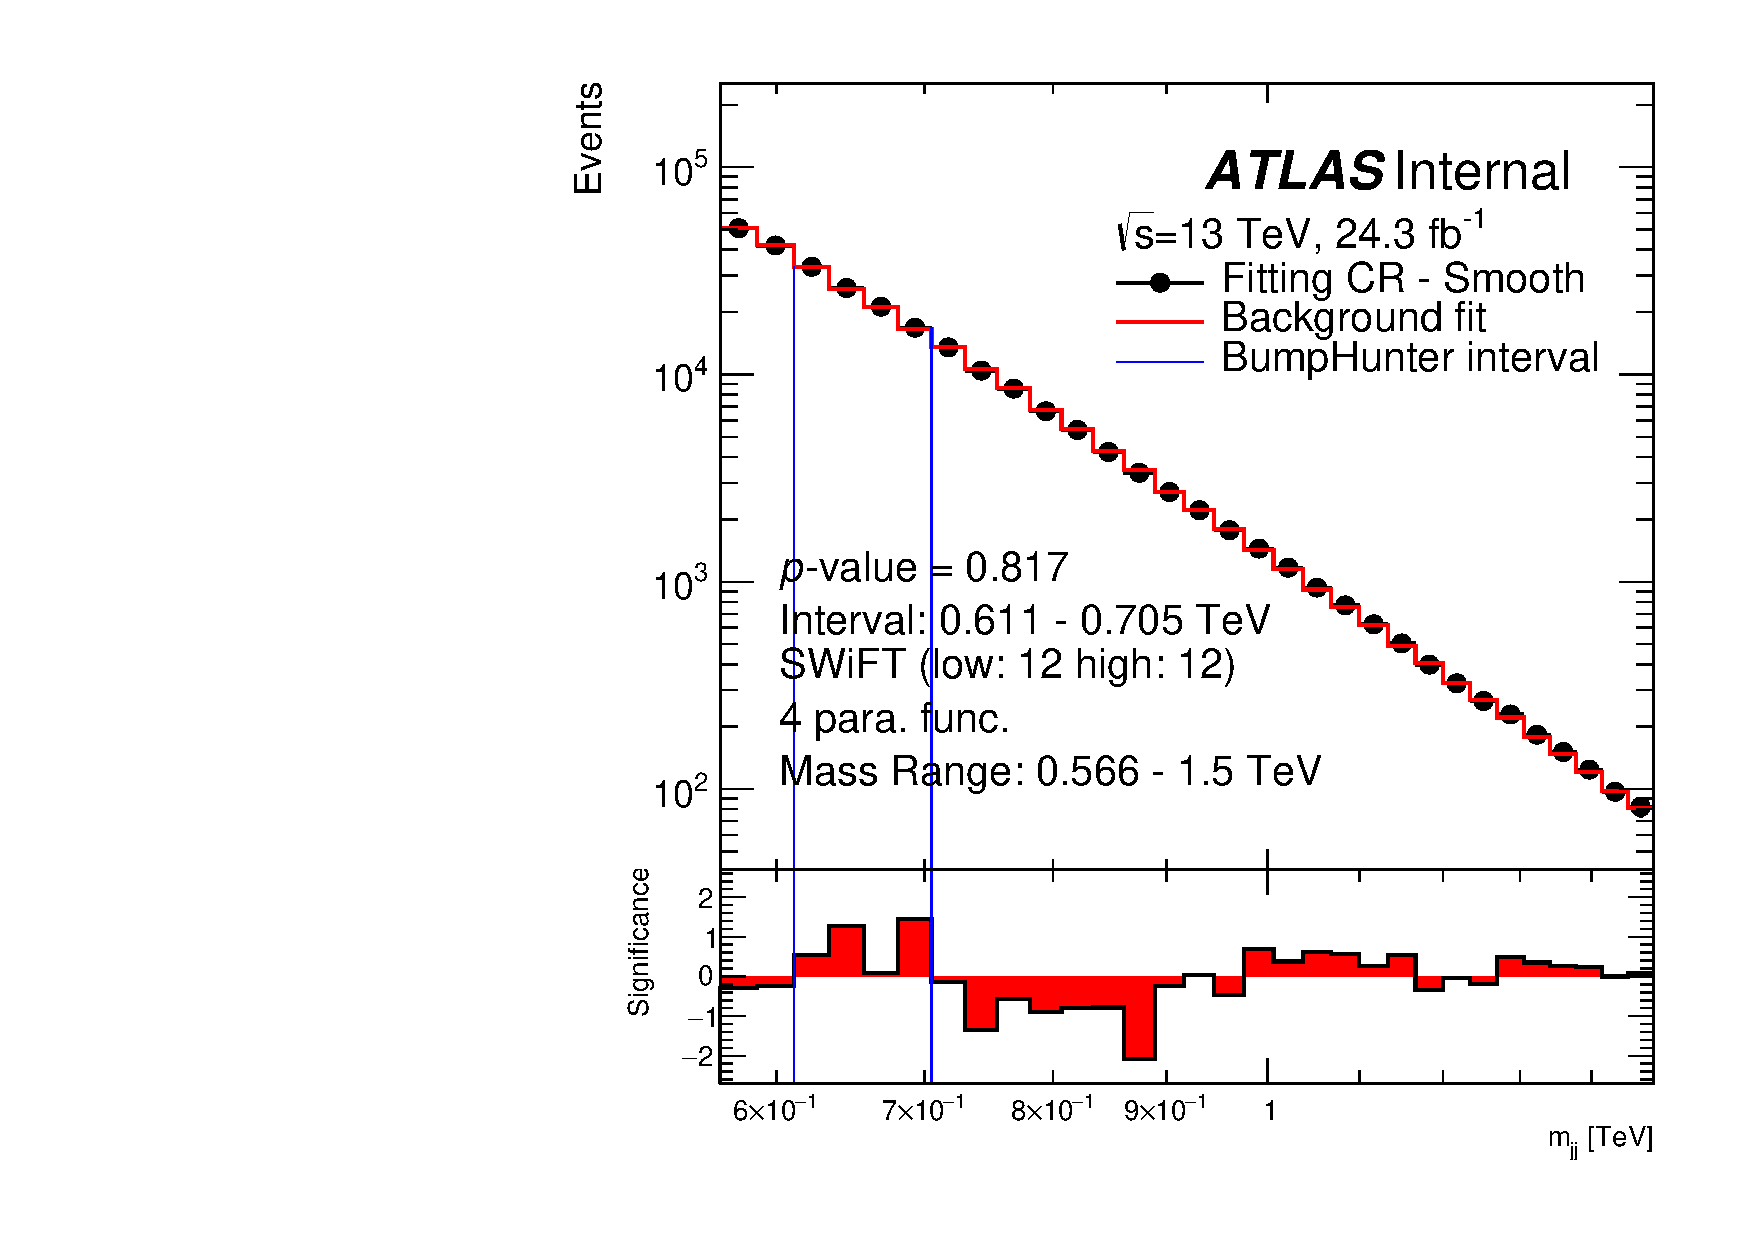
\includegraphics[width=0.48\linewidth, angle=0]{figs/Dibjet/LowMass/FitStudy_min566/bhFit_corrFitCR_smooth_4para_low12_high12.pdf}
}
\subcaptionbox{4 parameter fit, $wHW$ = 10} {
  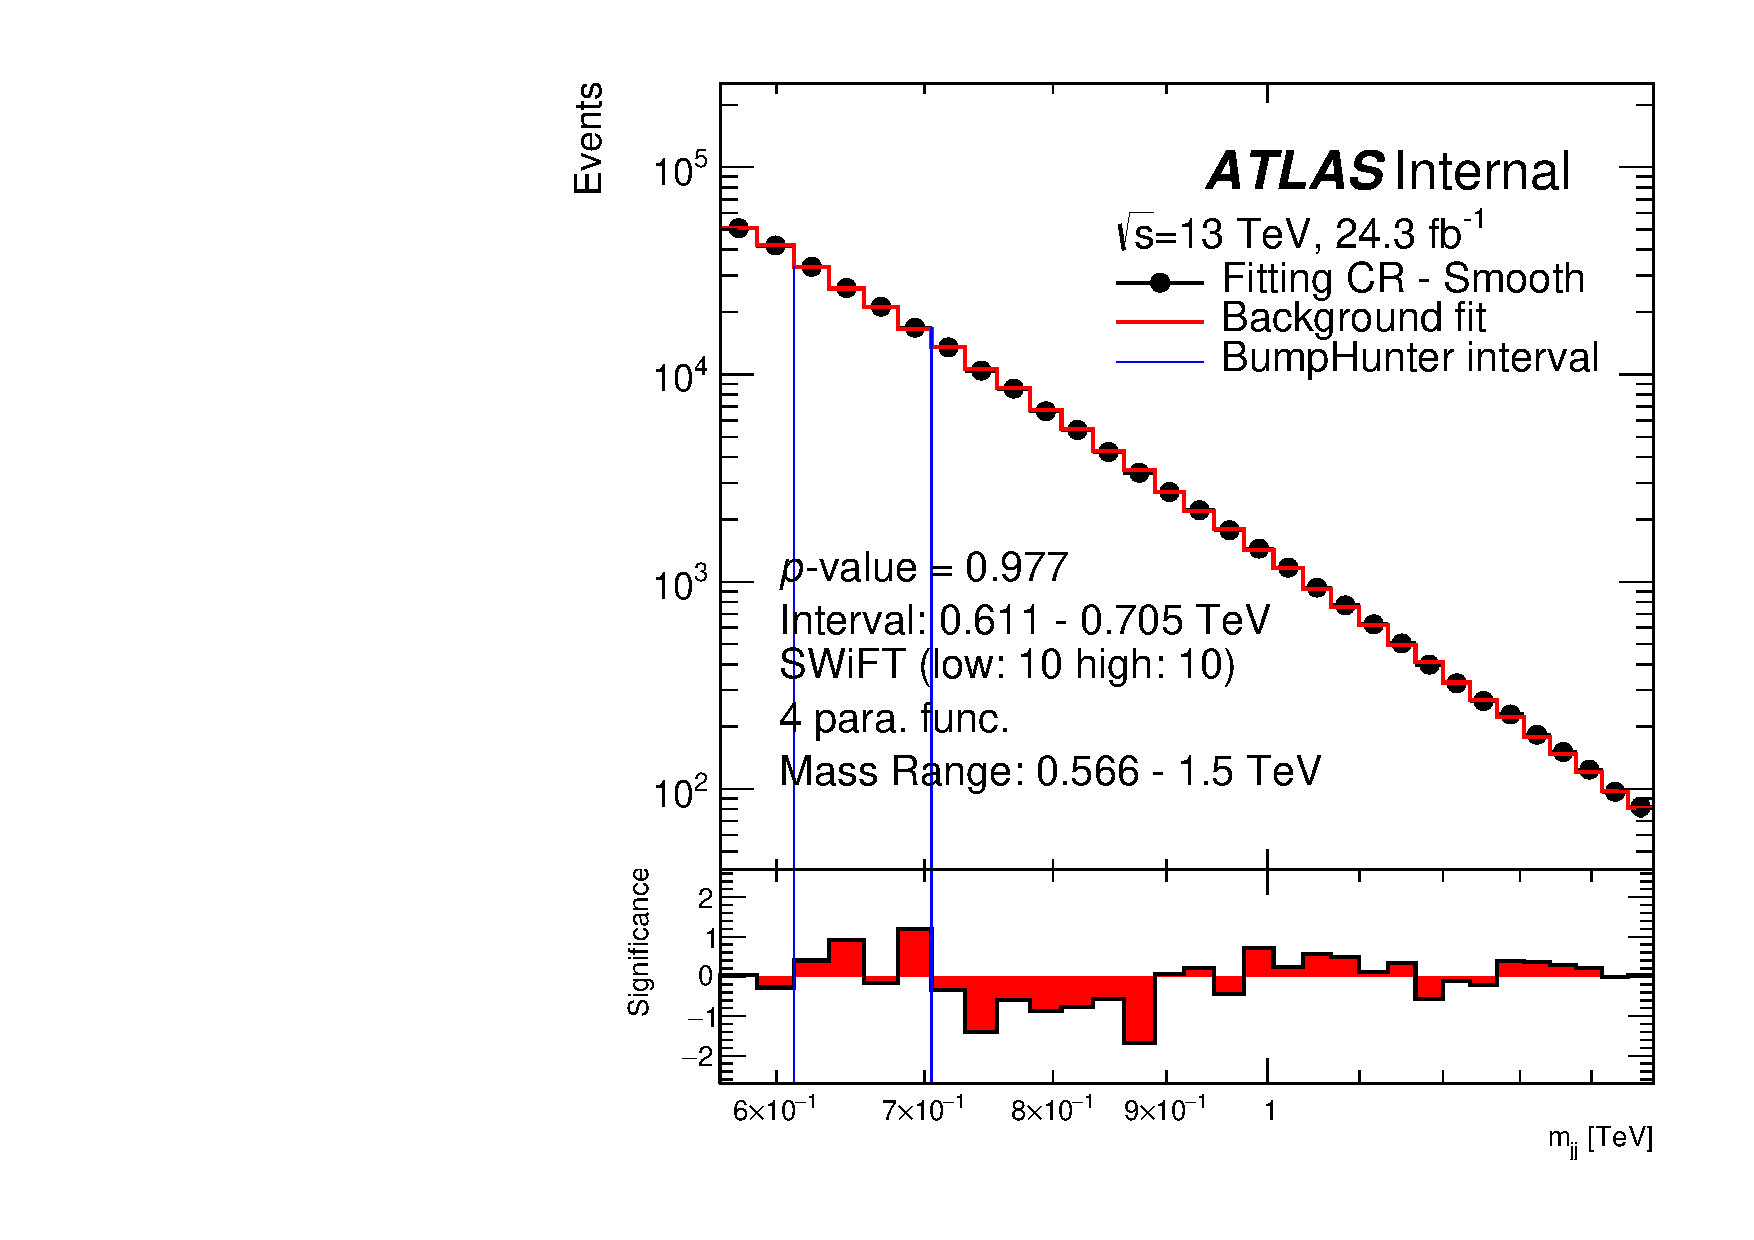
\includegraphics[width=0.48\linewidth, angle=0]{figs/Dibjet/LowMass/FitStudy_min566/bhFit_corrFitCR_smooth_4para_low10_high10.pdf}
}
\caption[Figure~\ref{fig:bhFit_lm_corrFitCR_smooth} for all SWiFt configurations using the 4 parameter dijet fit function..]
        {\label{fig:app-bhFit_lm_corrFitCR_smooth_4para}
        Figure~\ref{fig:bhFit_lm_corrFitCR_smooth} for all SWiFt configurations using the 4 parameter dijet fit function..
          The SWiFt search phase run on the smooth dijet mass spectrum from the fit control region for the \lm{} data-set.
          The SWiFt configurations considered use the 4 parameter dijet fit function for a window half-width ($wHW$) range of 10 to 16.
  
}    
\end{figure}
\begin{figure}
\captionsetup[subfigure]{aboveskip=0pt,justification=centering}
\subcaptionbox{5 parameter fit, $wHW$ = 16} {
  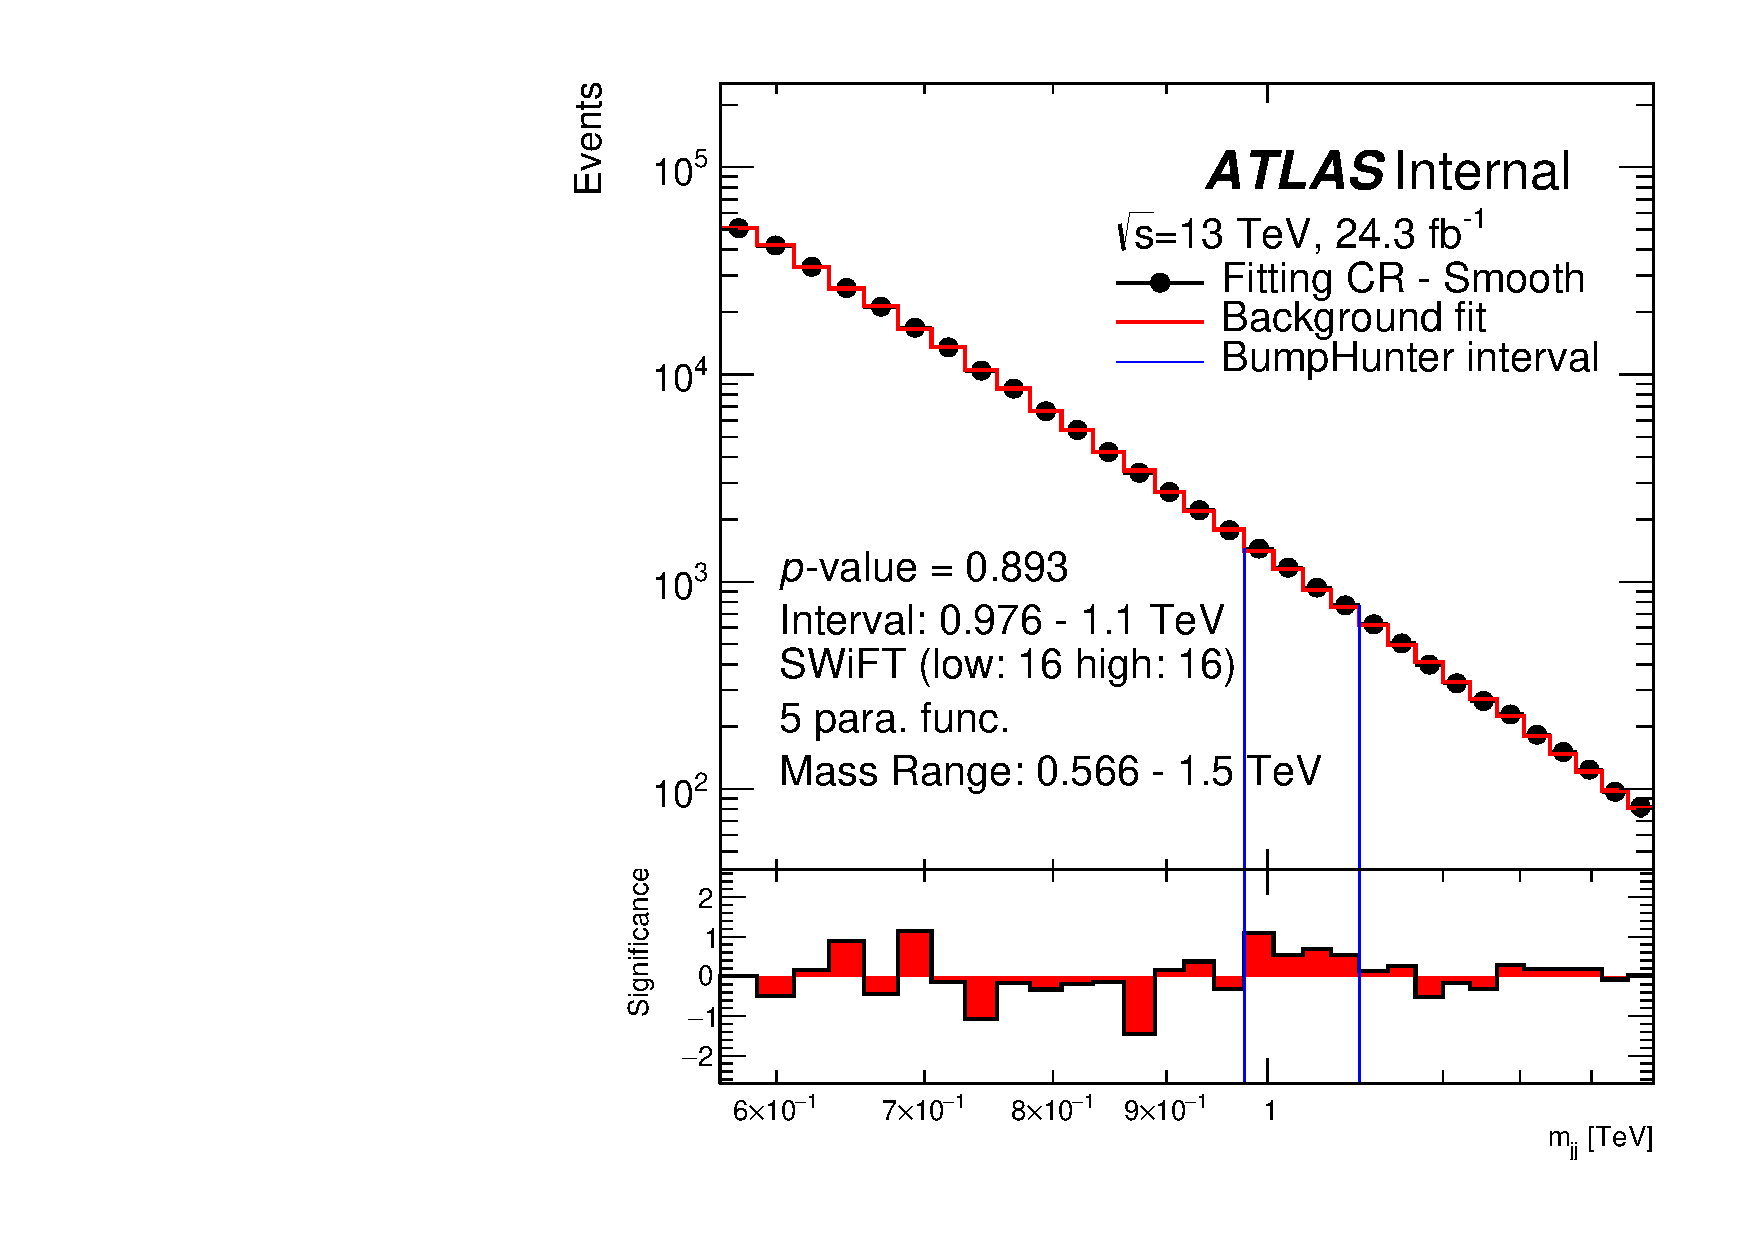
\includegraphics[width=0.48\linewidth, angle=0]{figs/Dibjet/LowMass/FitStudy_min566/bhFit_corrFitCR_smooth_5para_low16_high16.pdf}
}
\subcaptionbox{5 parameter fit, $wHW$ = 14} {
  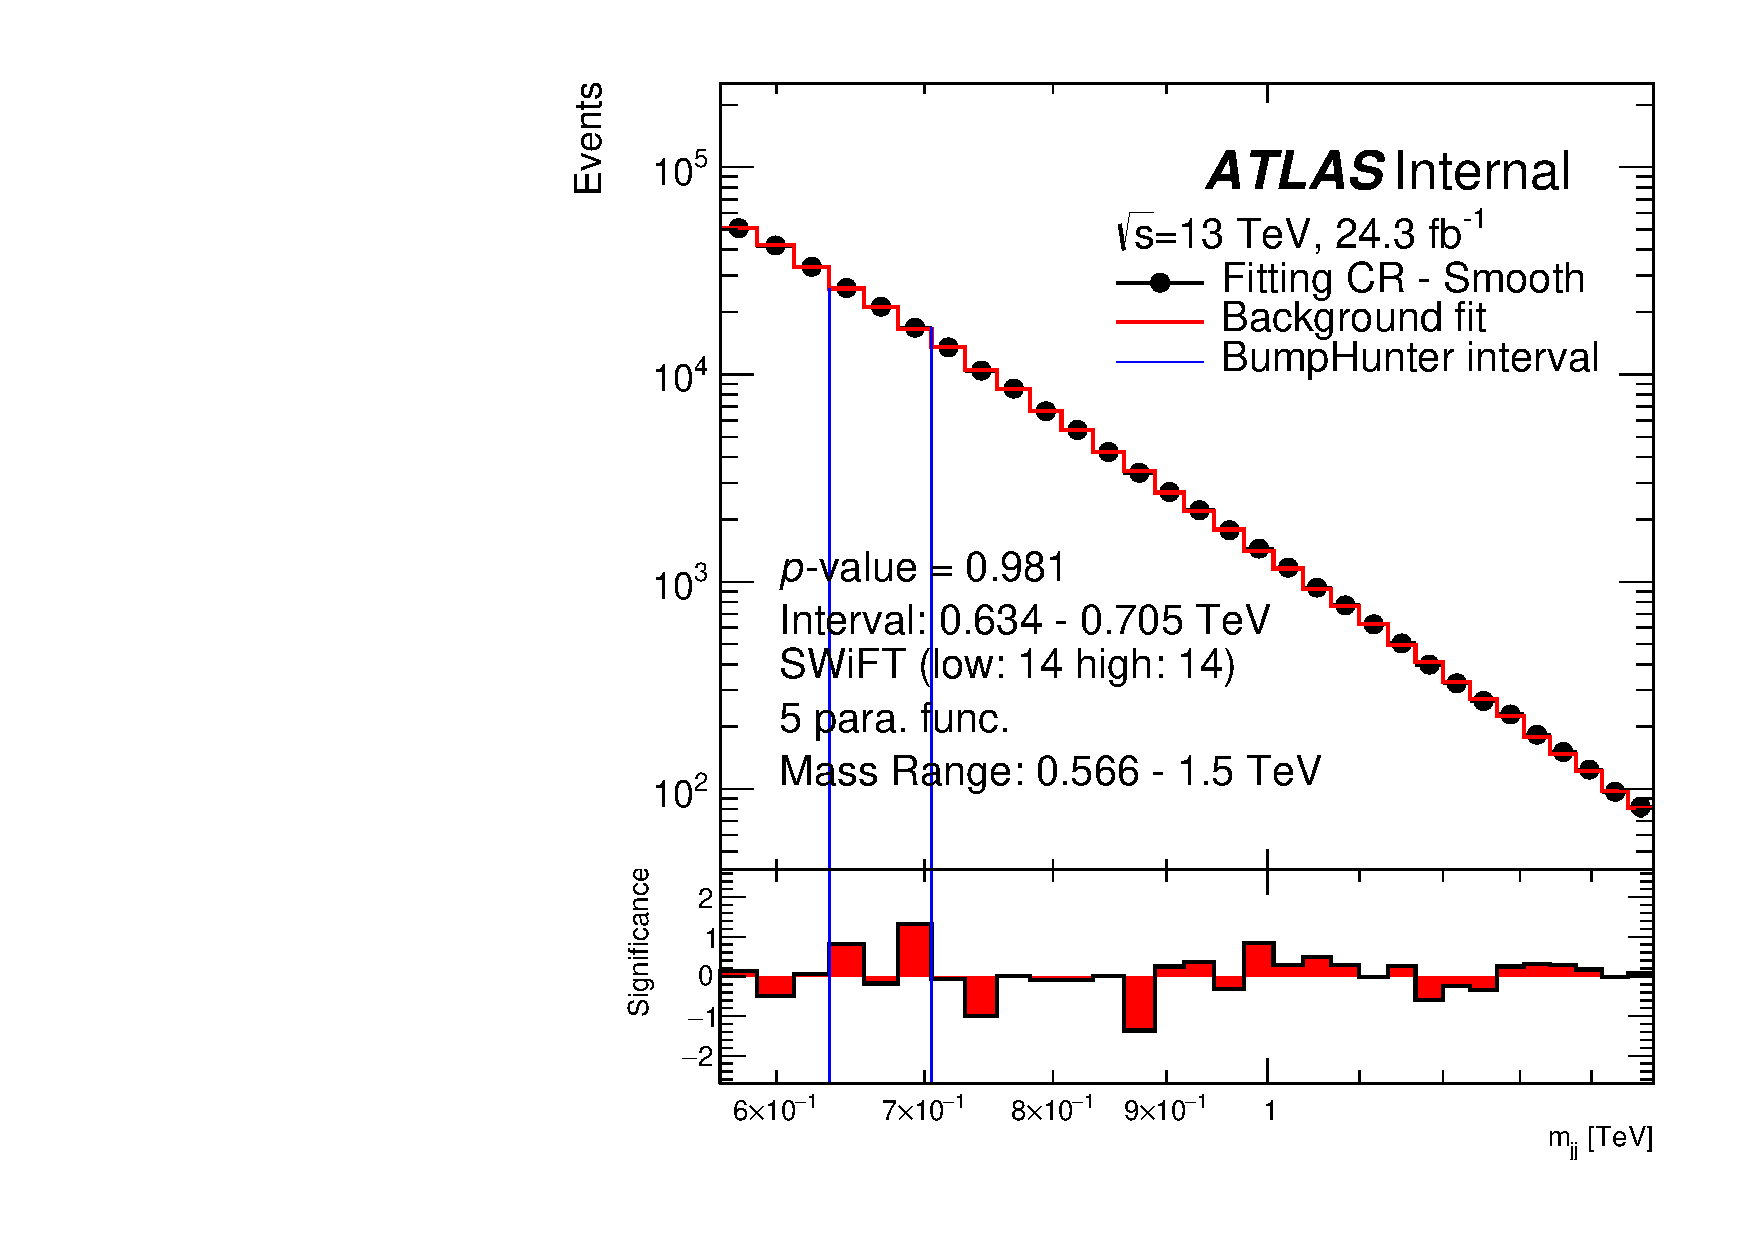
\includegraphics[width=0.48\linewidth, angle=0]{figs/Dibjet/LowMass/FitStudy_min566/bhFit_corrFitCR_smooth_5para_low14_high14.pdf}
}
\subcaptionbox{5 parameter fit, $wHW$ = 12} {
  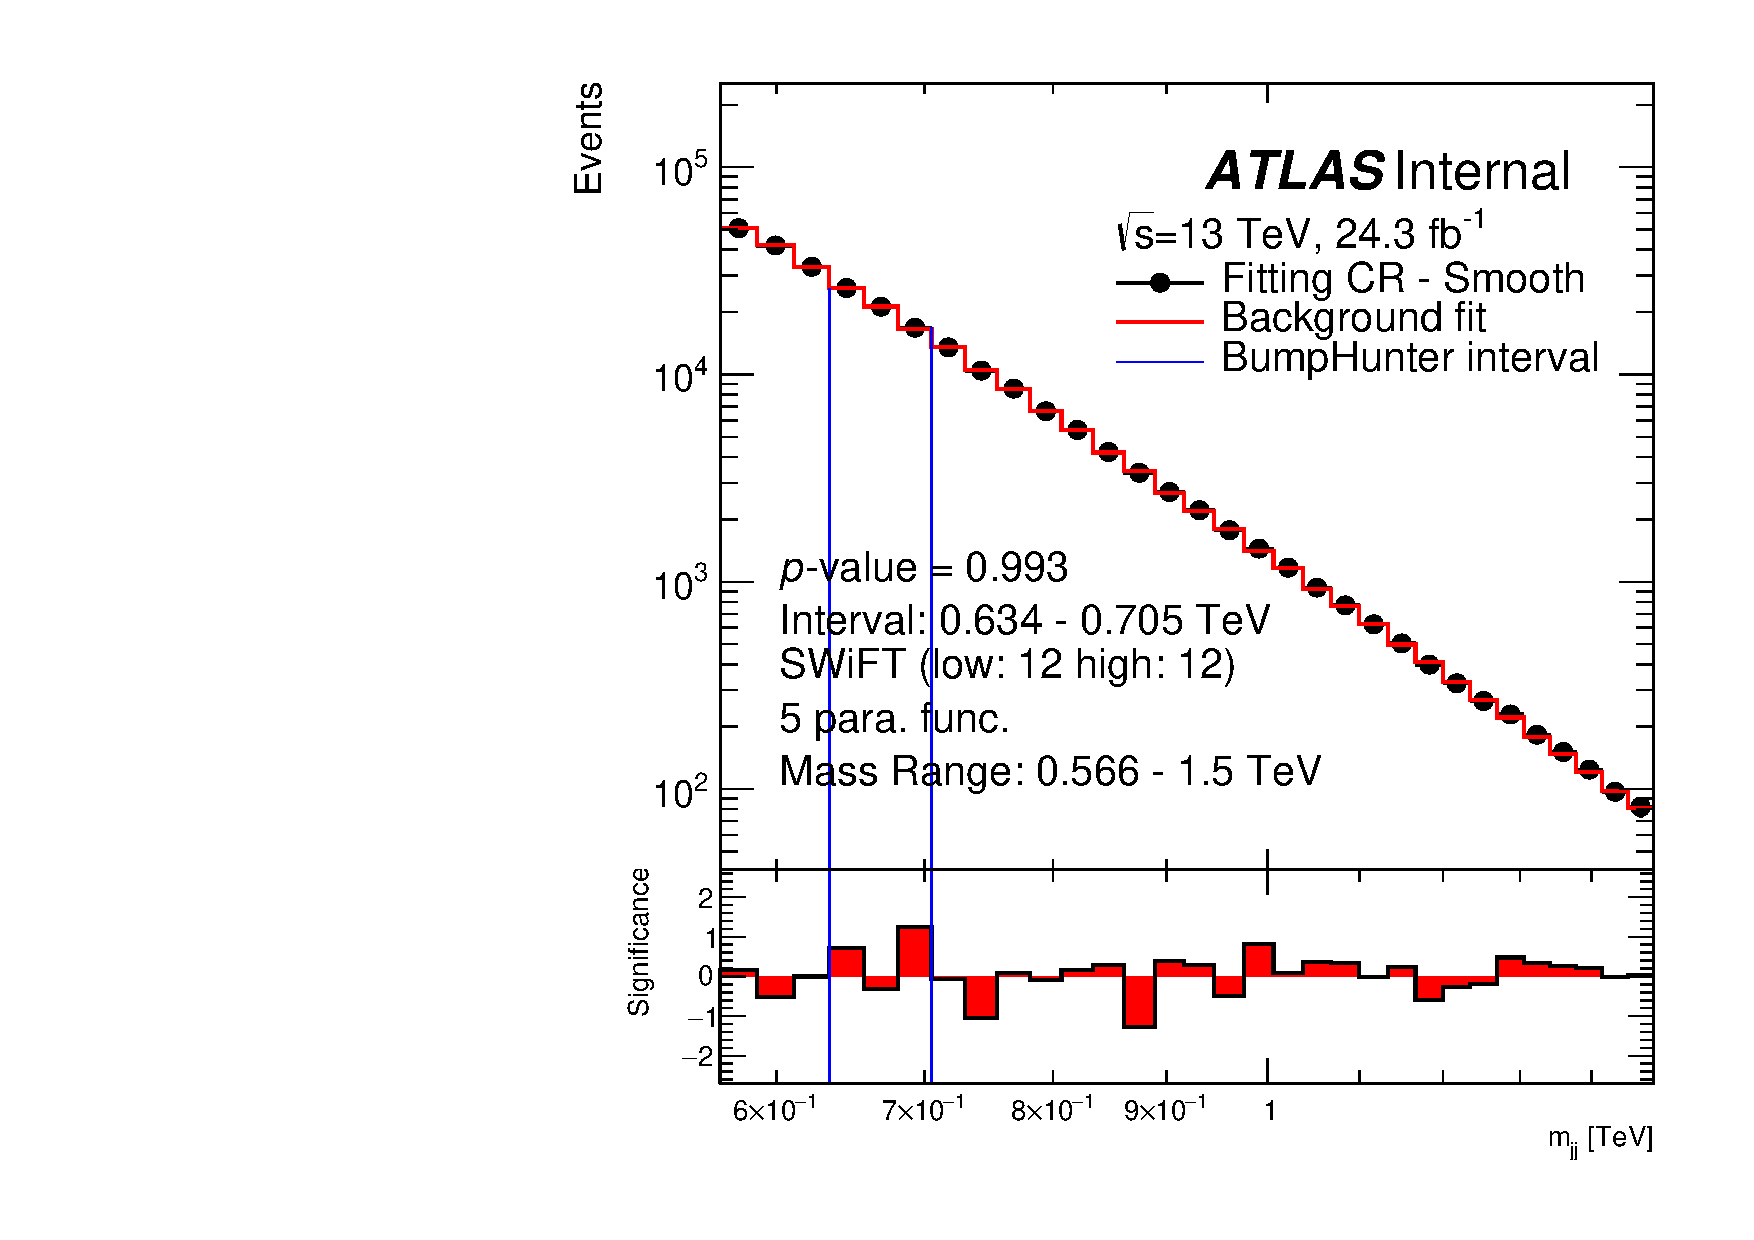
\includegraphics[width=0.48\linewidth, angle=0]{figs/Dibjet/LowMass/FitStudy_min566/bhFit_corrFitCR_smooth_5para_low12_high12.pdf}
}
\subcaptionbox{5 parameter fit, $wHW$ = 10} {
  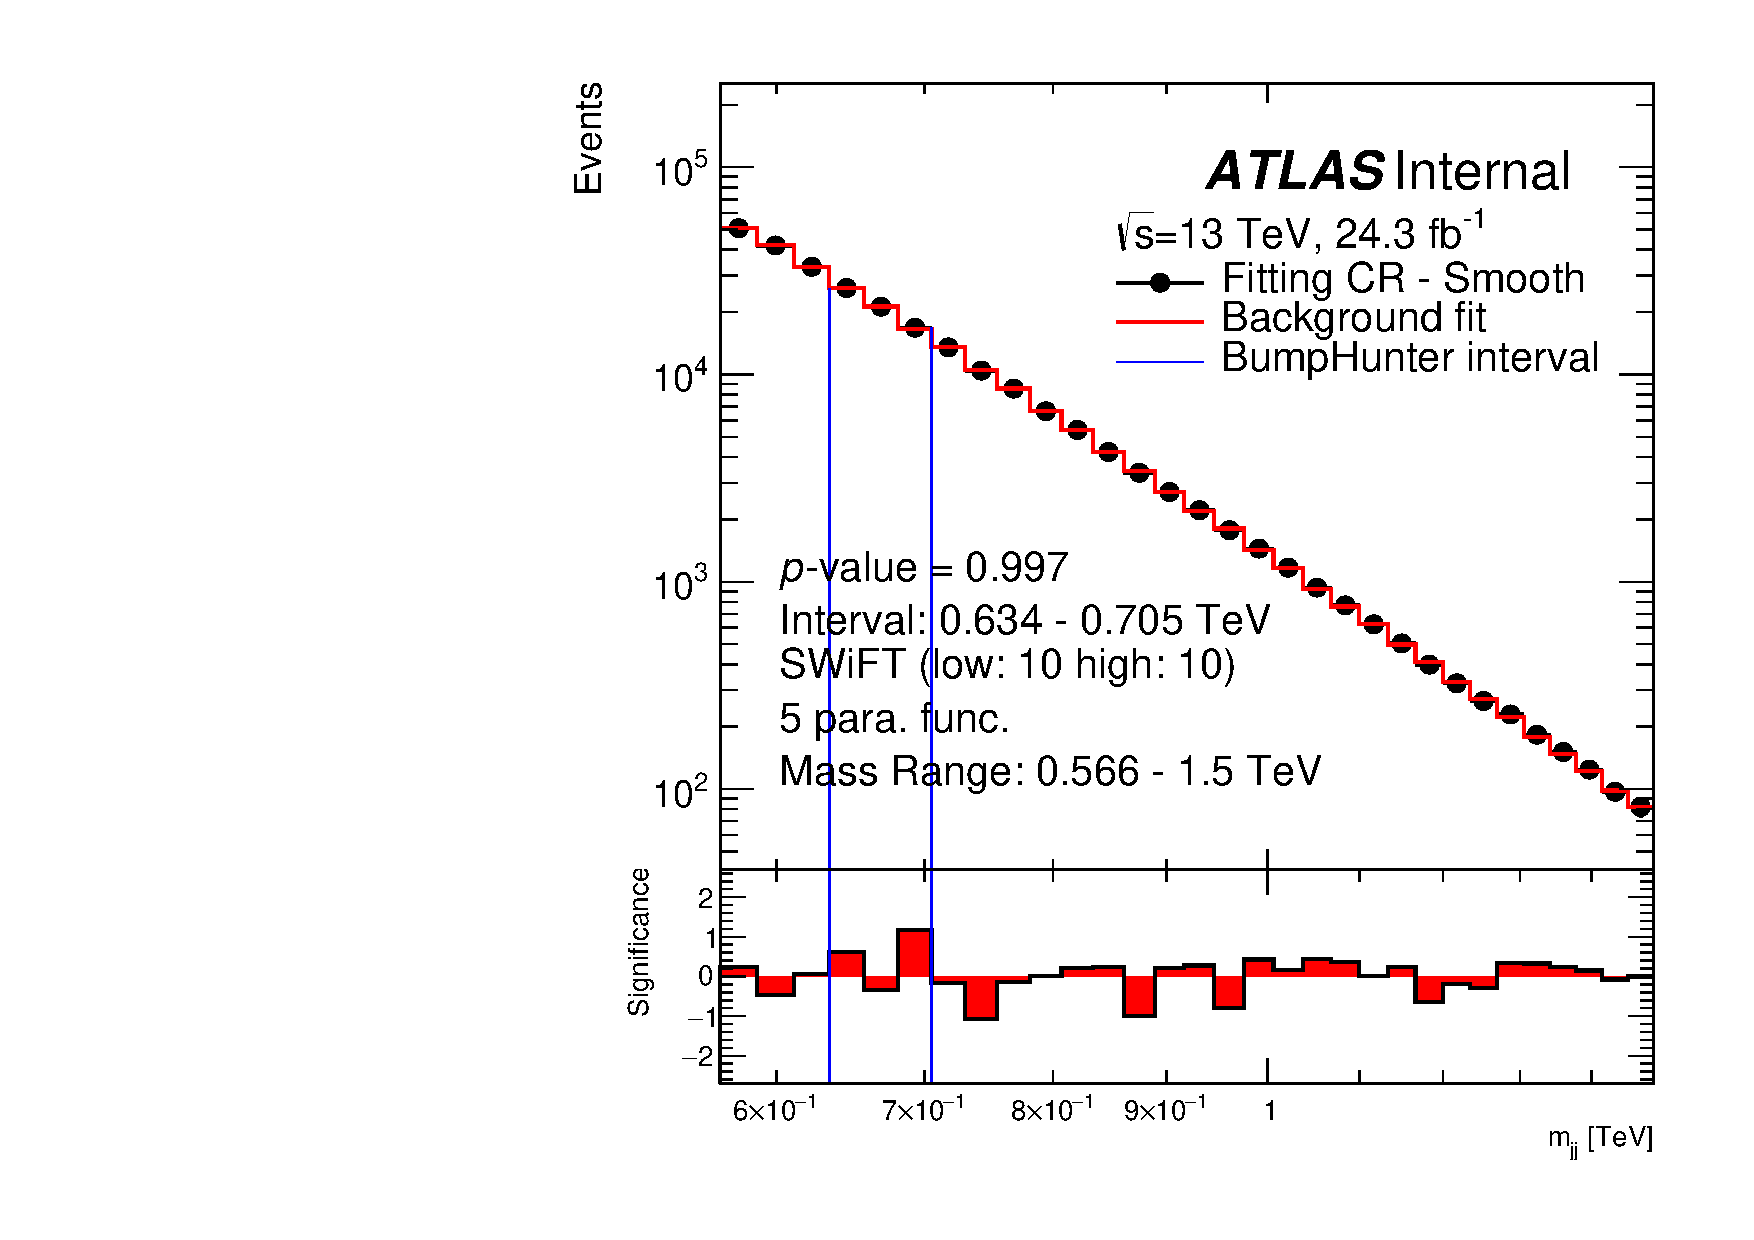
\includegraphics[width=0.48\linewidth, angle=0]{figs/Dibjet/LowMass/FitStudy_min566/bhFit_corrFitCR_smooth_5para_low10_high10.pdf}
}
\vspace{10pt}
\caption[Figure~\ref{fig:bhFit_lm_corrFitCR_smooth} for all SWiFt configurations using the 5 parameter dijet fit function..]
        {\label{fig:app-bhFit_lm_corrFitCR_smooth_5para}
        Figure~\ref{fig:bhFit_lm_corrFitCR_smooth} for all SWiFt configurations using the 5 parameter dijet fit function..
          The SWiFt search phase run on the smooth dijet mass spectrum from the fit control region for the \lm{} data-set.
          The SWiFt configurations considered use the 5 parameter dijet fit function for a window half-width ($wHW$) range of 10 to 16.
  
}    
\end{figure}

\clearpage

\section{Figure~\ref{fig:bhFit_lm_corrFitCR_dataLike} for all SWiFt configurations}
\vspace{5em}

\begin{figure}[!htb]
\captionsetup[subfigure]{aboveskip=0pt,justification=centering}
\centering
\subcaptionbox{4 parameter fit, $wHW$ = 16} {
  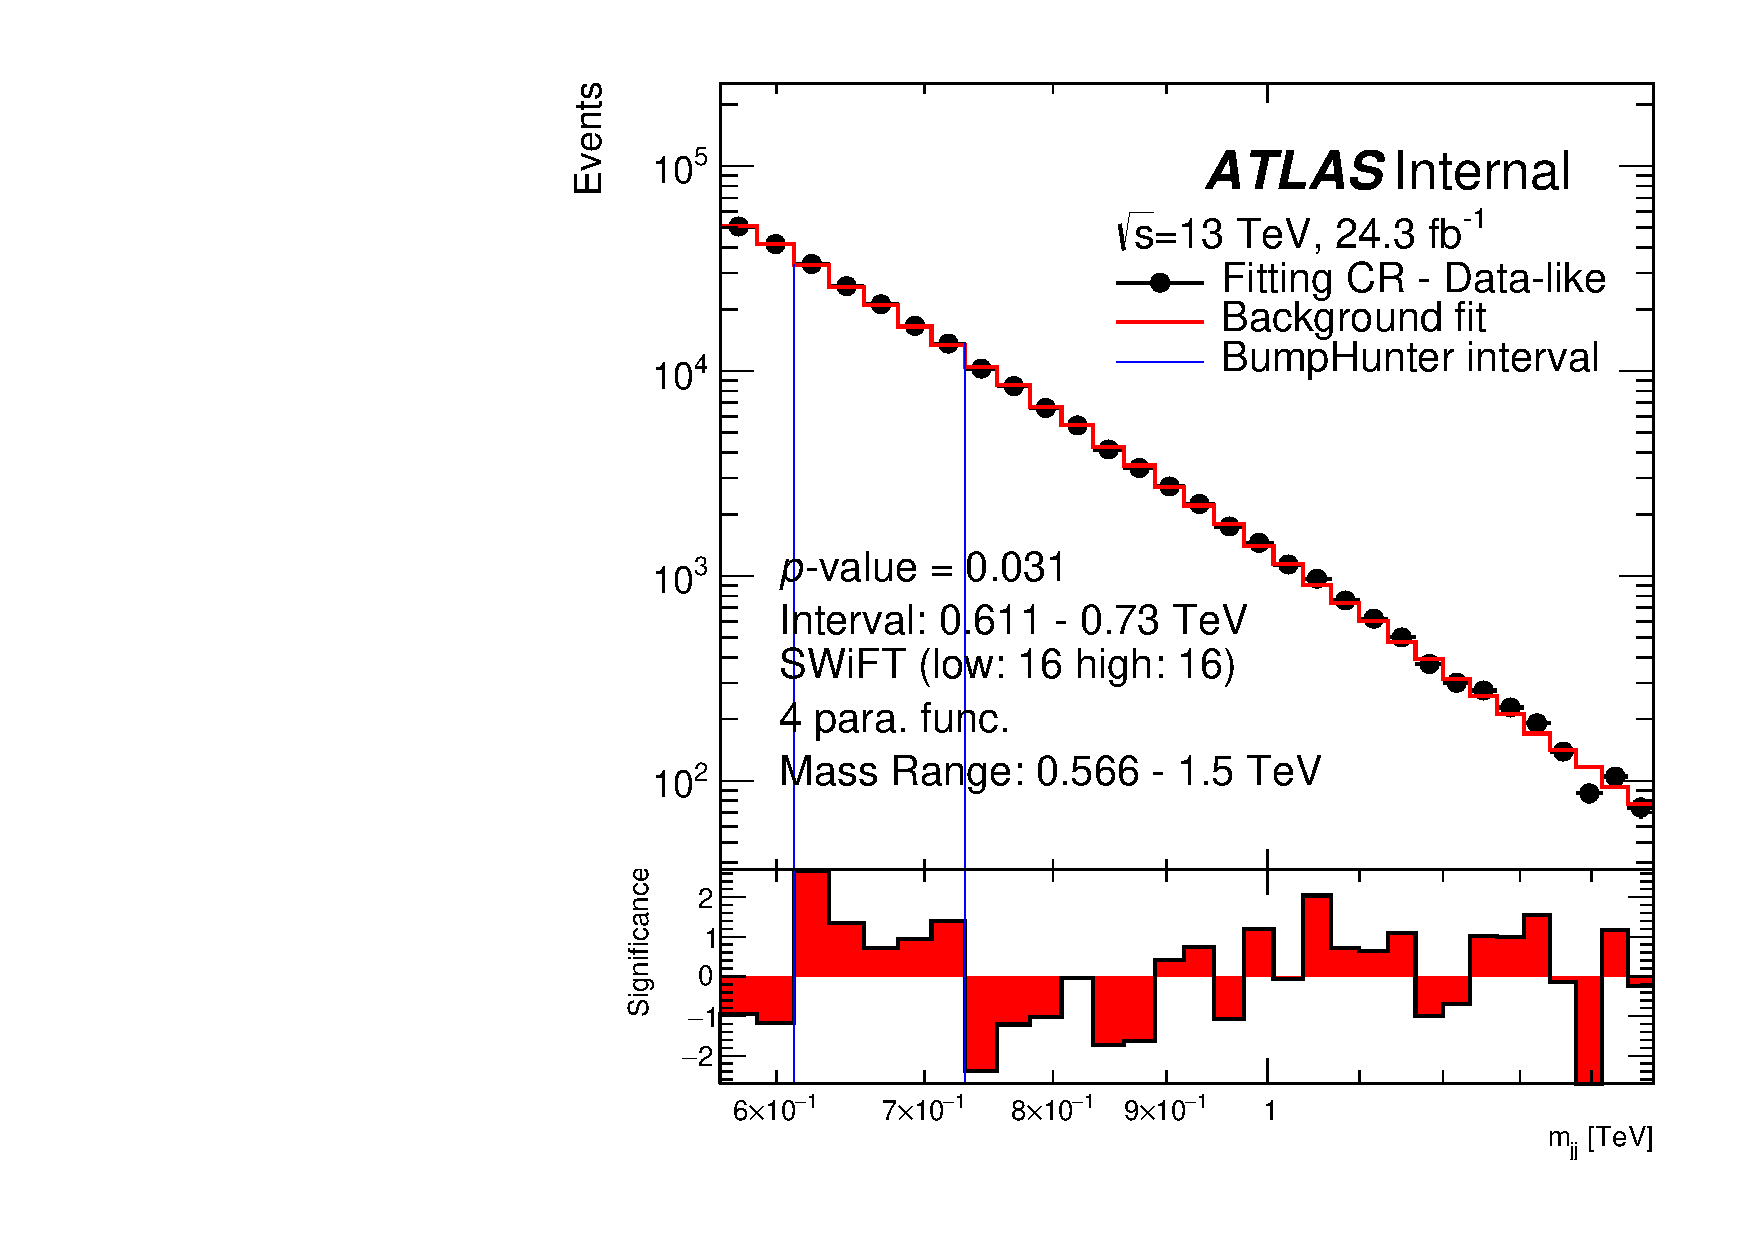
\includegraphics[width=0.48\linewidth, angle=0]{figs/Dibjet/LowMass/FitStudy_min566/bhFit_corrFitCR_dataLike_v13_4para_low16_high16.pdf}
}
\subcaptionbox{4 parameter fit, $wHW$ = 14} {
  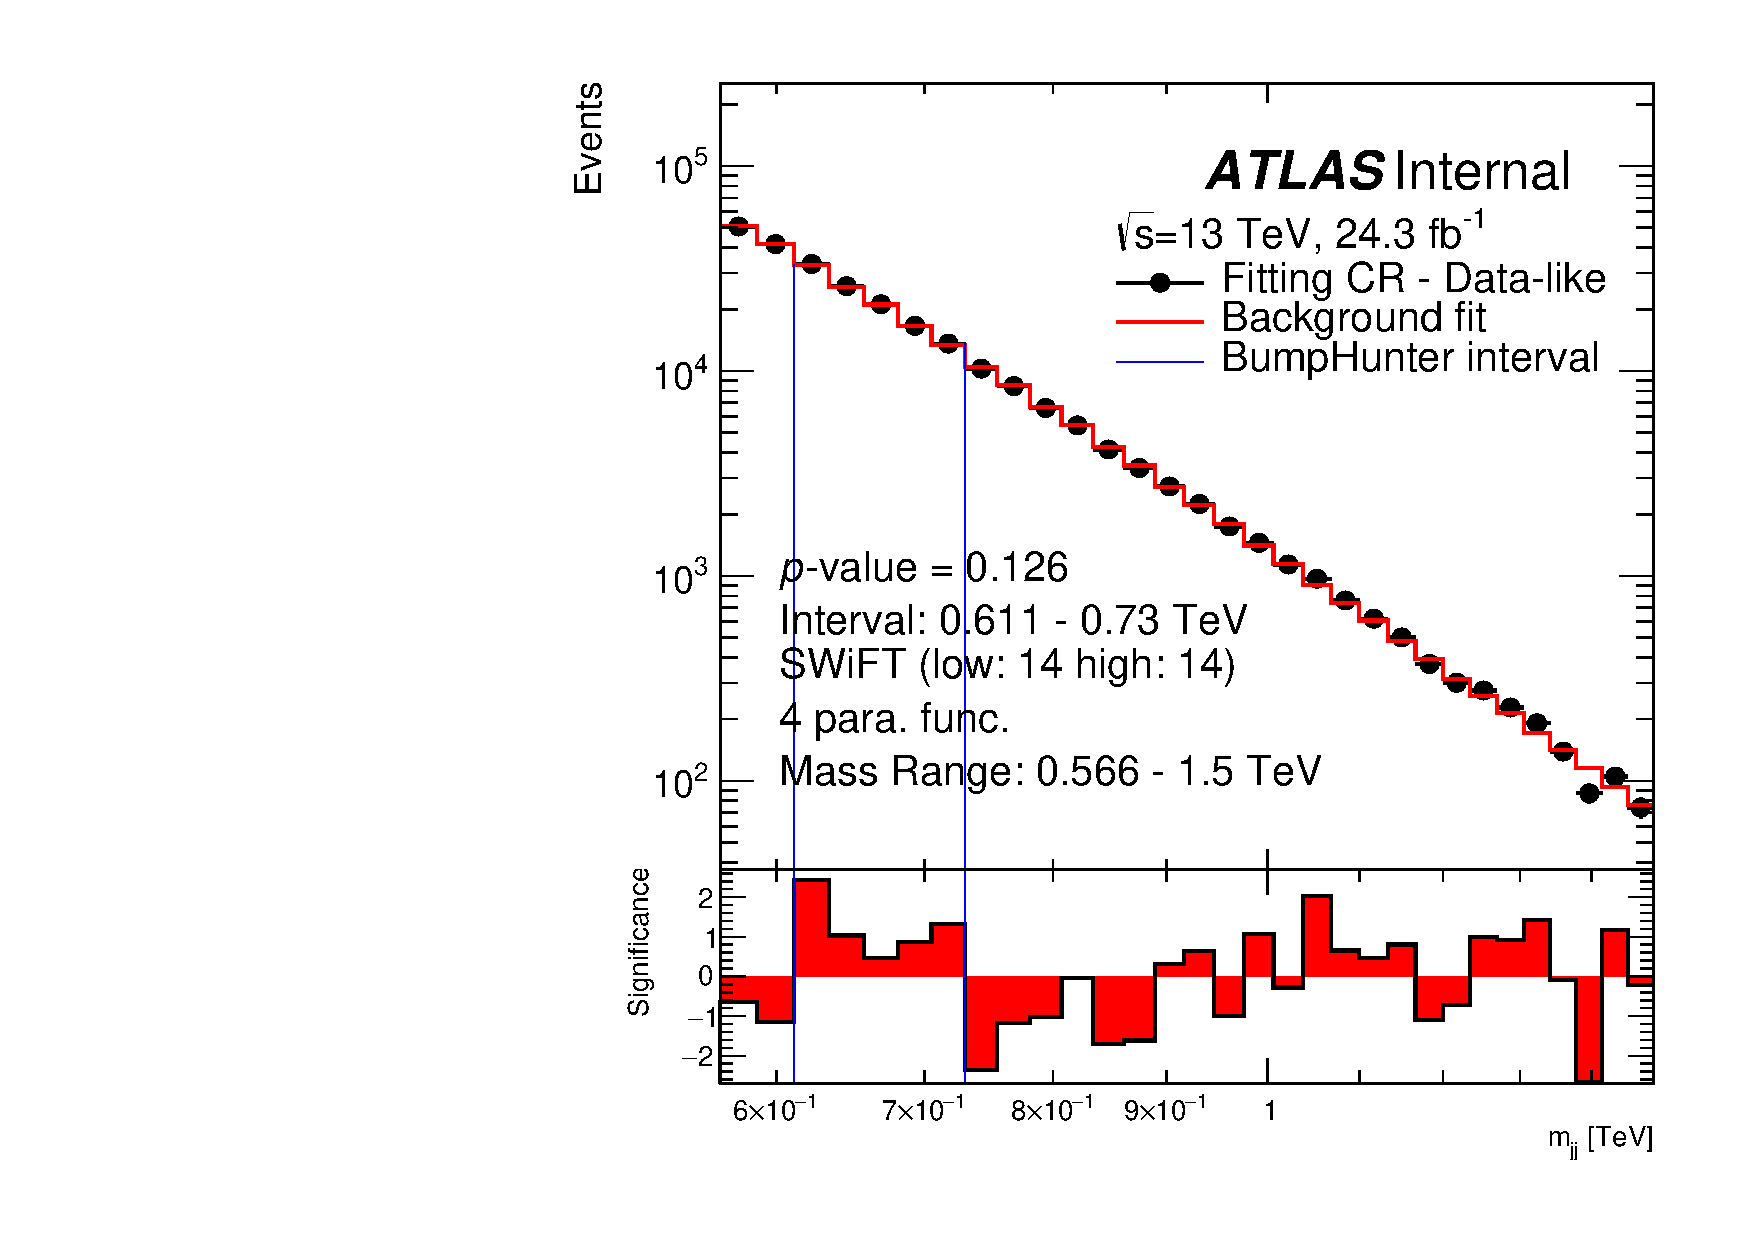
\includegraphics[width=0.48\linewidth, angle=0]{figs/Dibjet/LowMass/FitStudy_min566/bhFit_corrFitCR_dataLike_v13_4para_low14_high14.pdf}
}
\subcaptionbox{4 parameter fit, $wHW$ = 12} {
  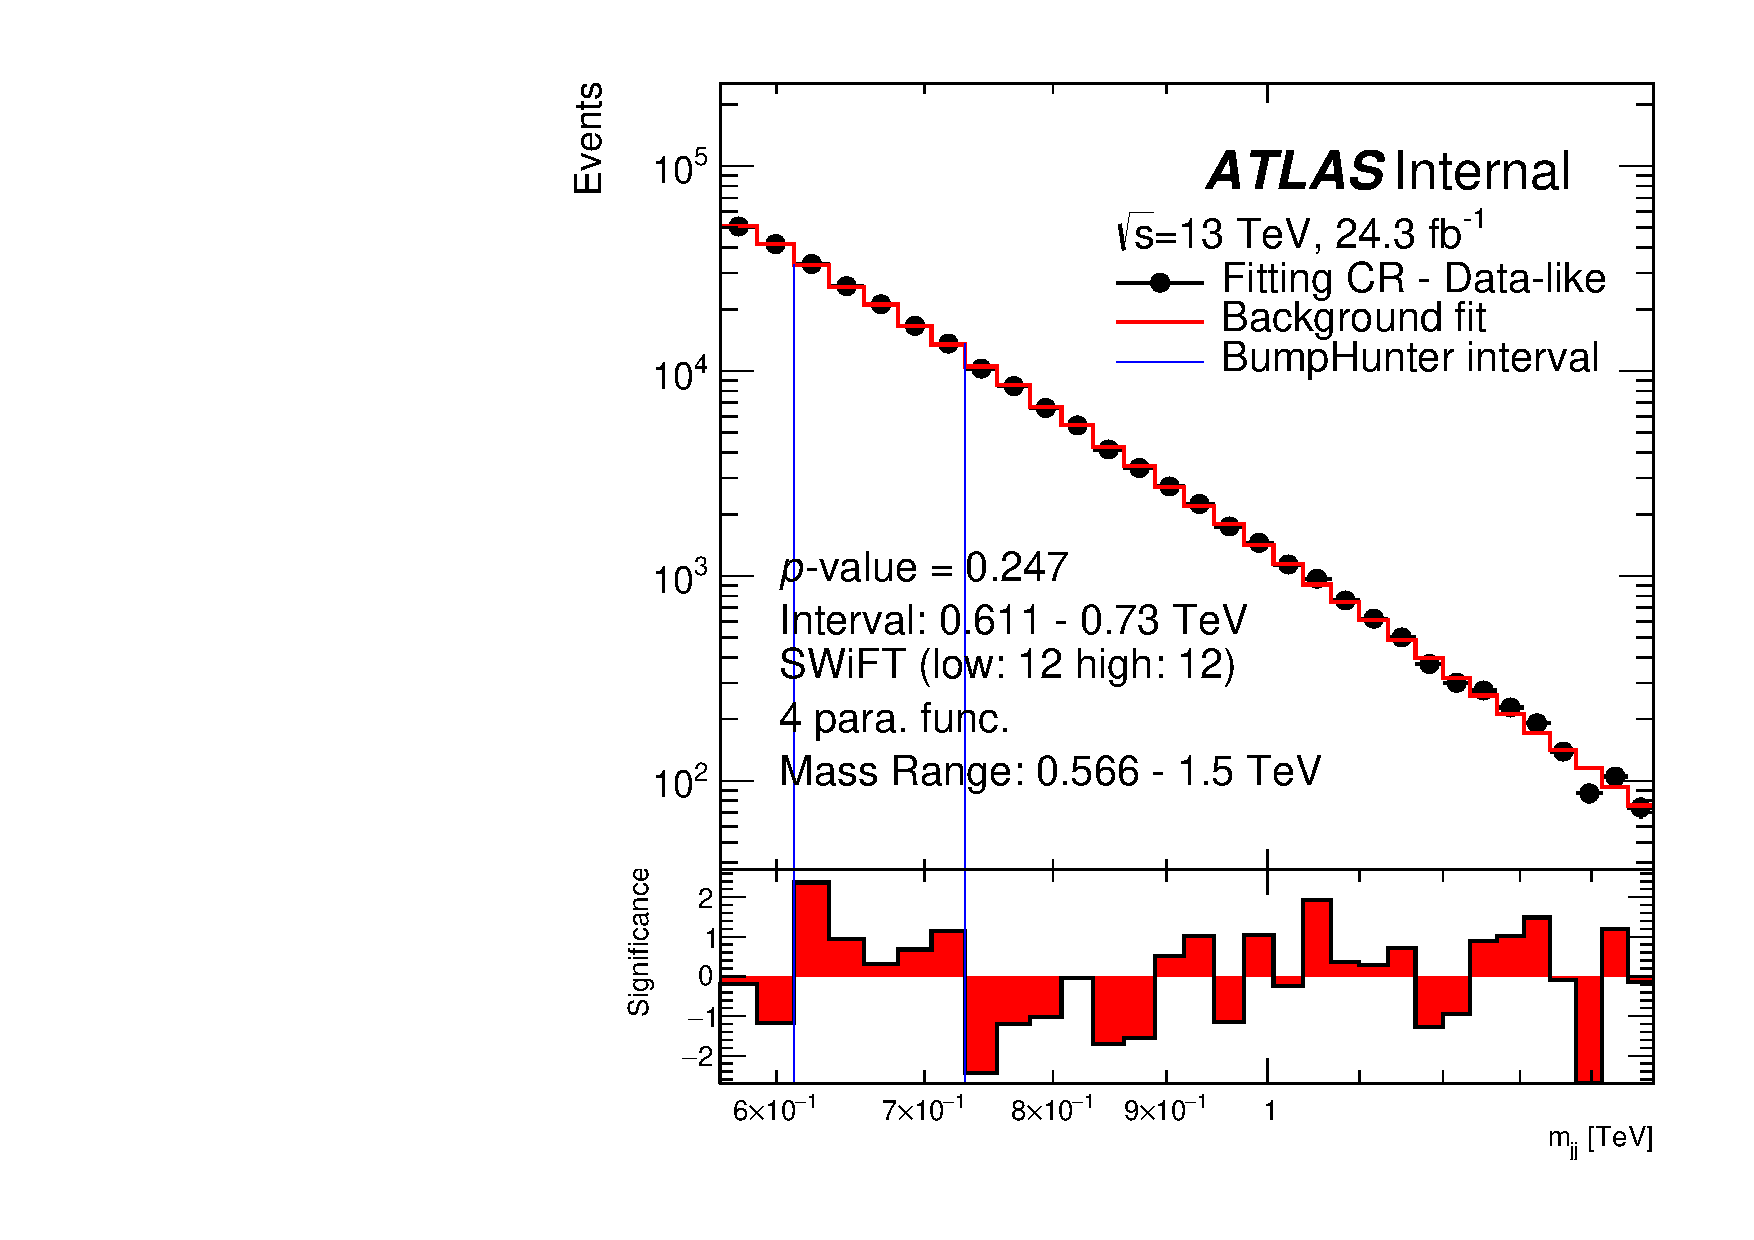
\includegraphics[width=0.48\linewidth, angle=0]{figs/Dibjet/LowMass/FitStudy_min566/bhFit_corrFitCR_dataLike_v13_4para_low12_high12.pdf}
}
\subcaptionbox{4 parameter fit, $wHW$ = 10} {
  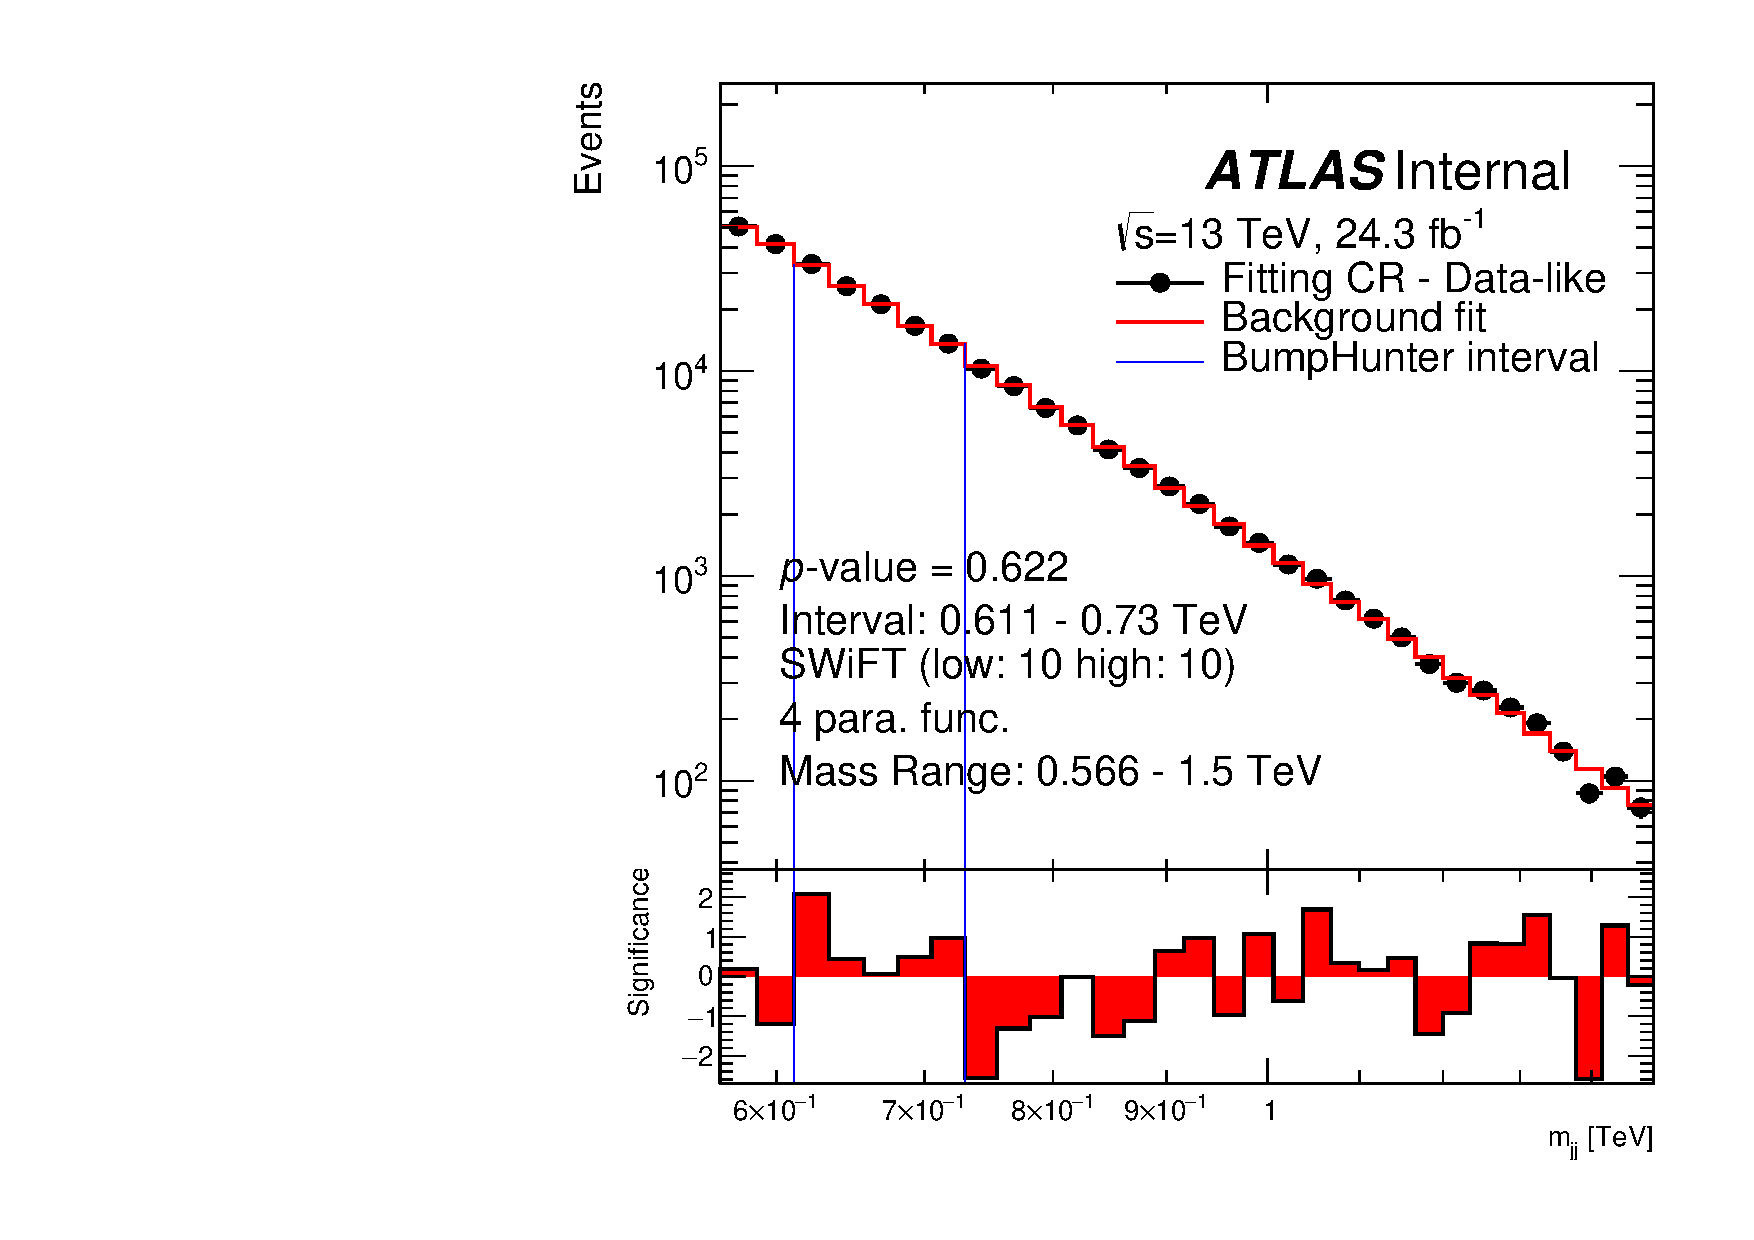
\includegraphics[width=0.48\linewidth, angle=0]{figs/Dibjet/LowMass/FitStudy_min566/bhFit_corrFitCR_dataLike_v13_4para_low10_high10.pdf}
}
\caption[Figure~\ref{fig:bhFit_lm_corrFitCR_dataLike} for all SWiFt configurations using the 4 parameter dijet fit function..]
{\label{fig:app-bhFit_lm_corrFitCR_dataLike_4para}
  Figure~\ref{fig:bhFit_lm_corrFitCR_dataLike} for all SWiFt configurations using the 4 parameter dijet fit function..
  The SWiFt search phase run on a data-like dijet mass spectrum
  from the fit control region for the \lm{} data-set.
  The SWiFt configurations considered use the 4 parameter dijet fit function for a window half-width ($wHW$) range of 10 to 16.
}
\end{figure}
\begin{figure}
\captionsetup[subfigure]{aboveskip=0pt,justification=centering}
\subcaptionbox{5 parameter fit, $wHW$ = 16} {
  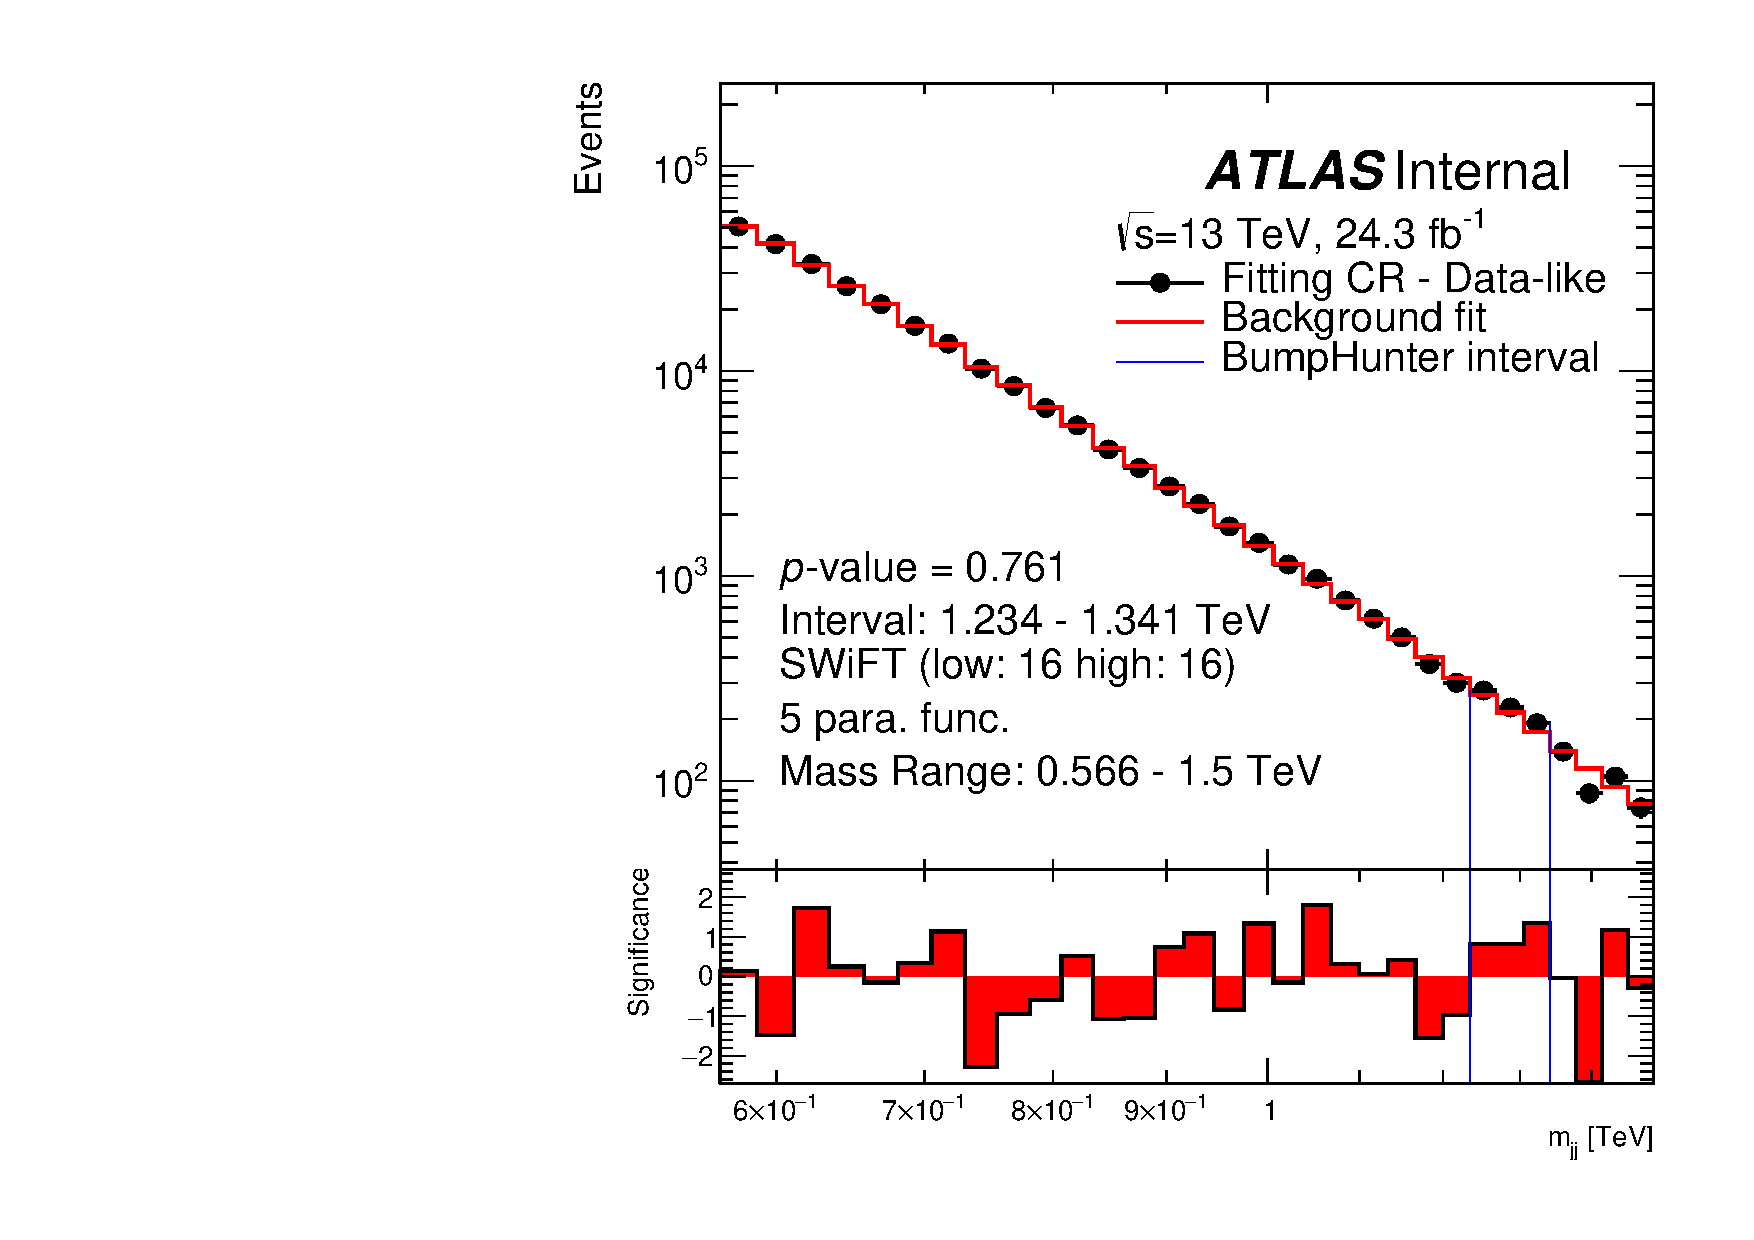
\includegraphics[width=0.48\linewidth, angle=0]{figs/Dibjet/LowMass/FitStudy_min566/bhFit_corrFitCR_dataLike_v13_5para_low16_high16.pdf}
}
\subcaptionbox{5 parameter fit, $wHW$ = 14} {
  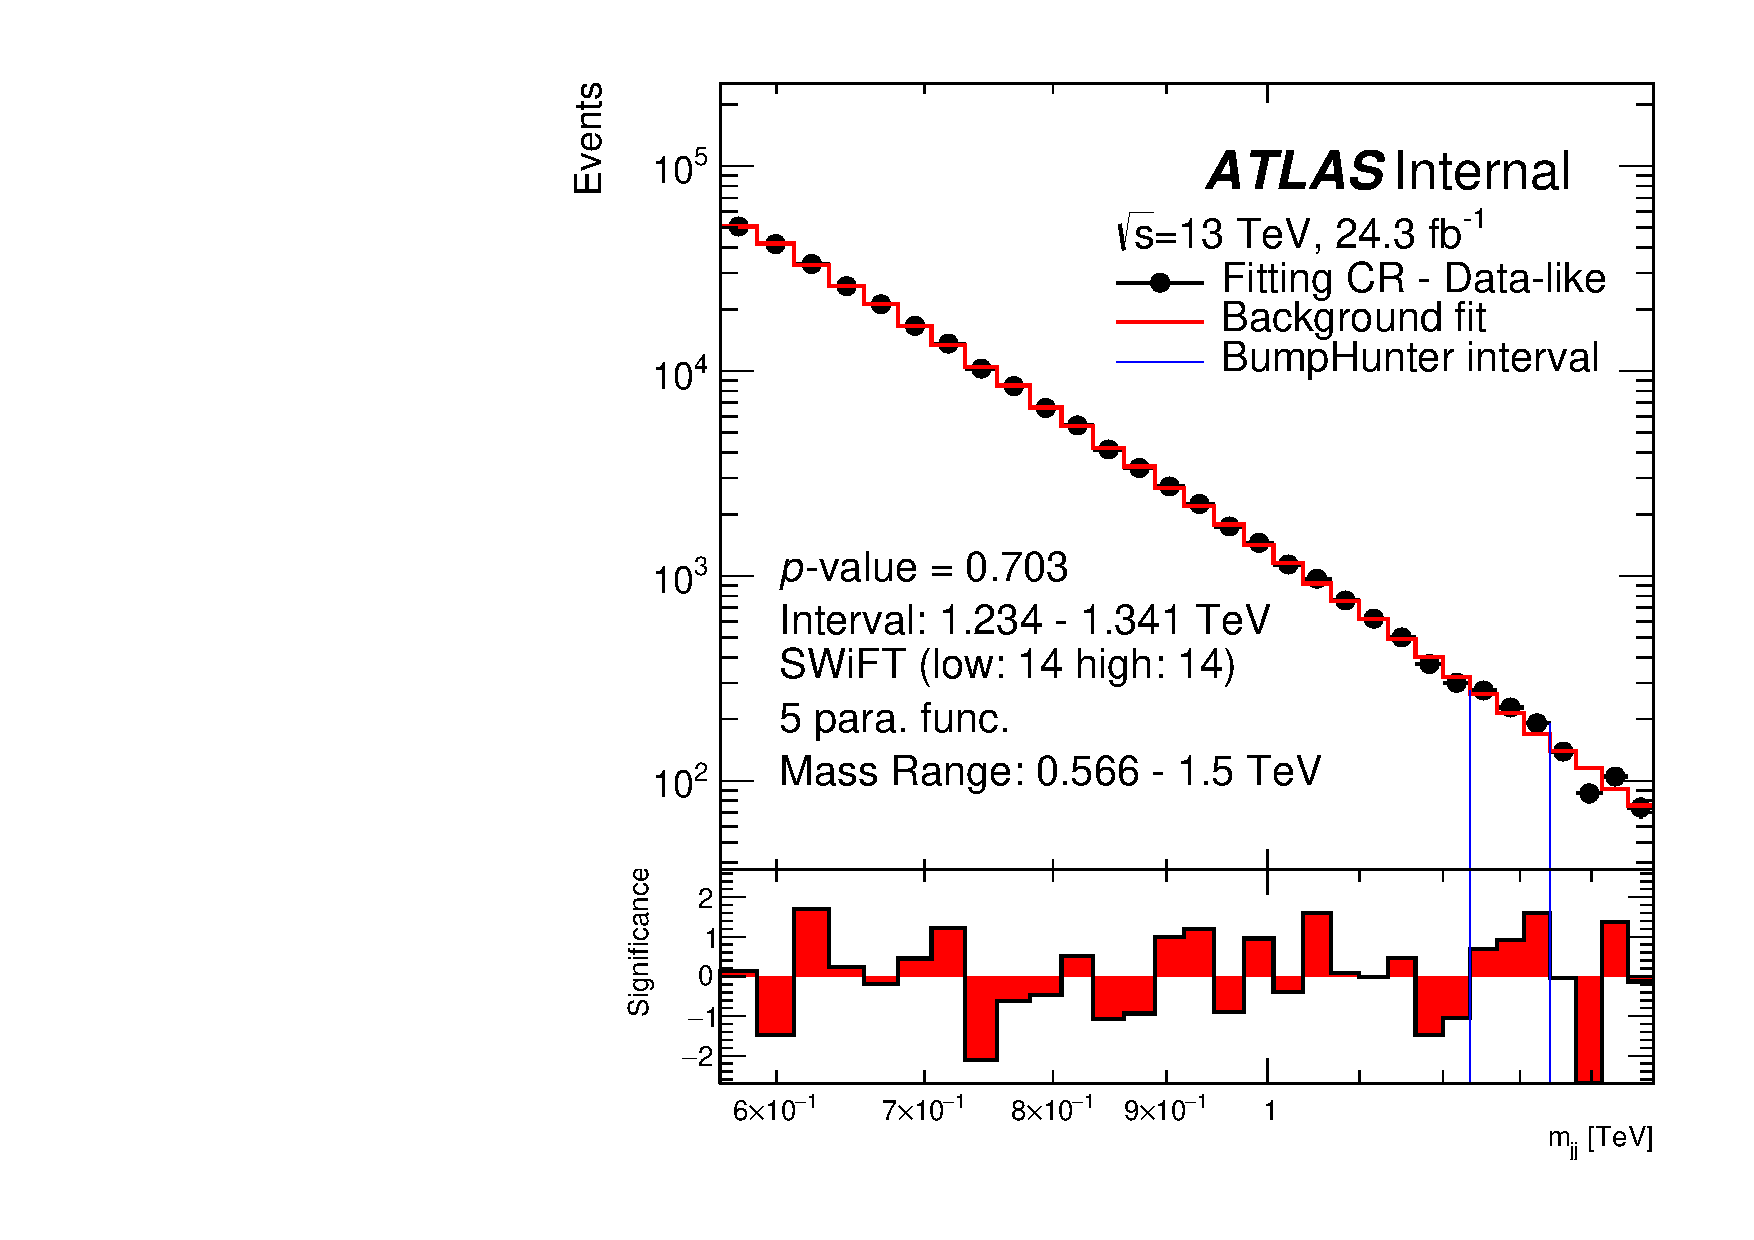
\includegraphics[width=0.48\linewidth, angle=0]{figs/Dibjet/LowMass/FitStudy_min566/bhFit_corrFitCR_dataLike_v13_5para_low14_high14.pdf}
}
\subcaptionbox{5 parameter fit, $wHW$ = 12} {
  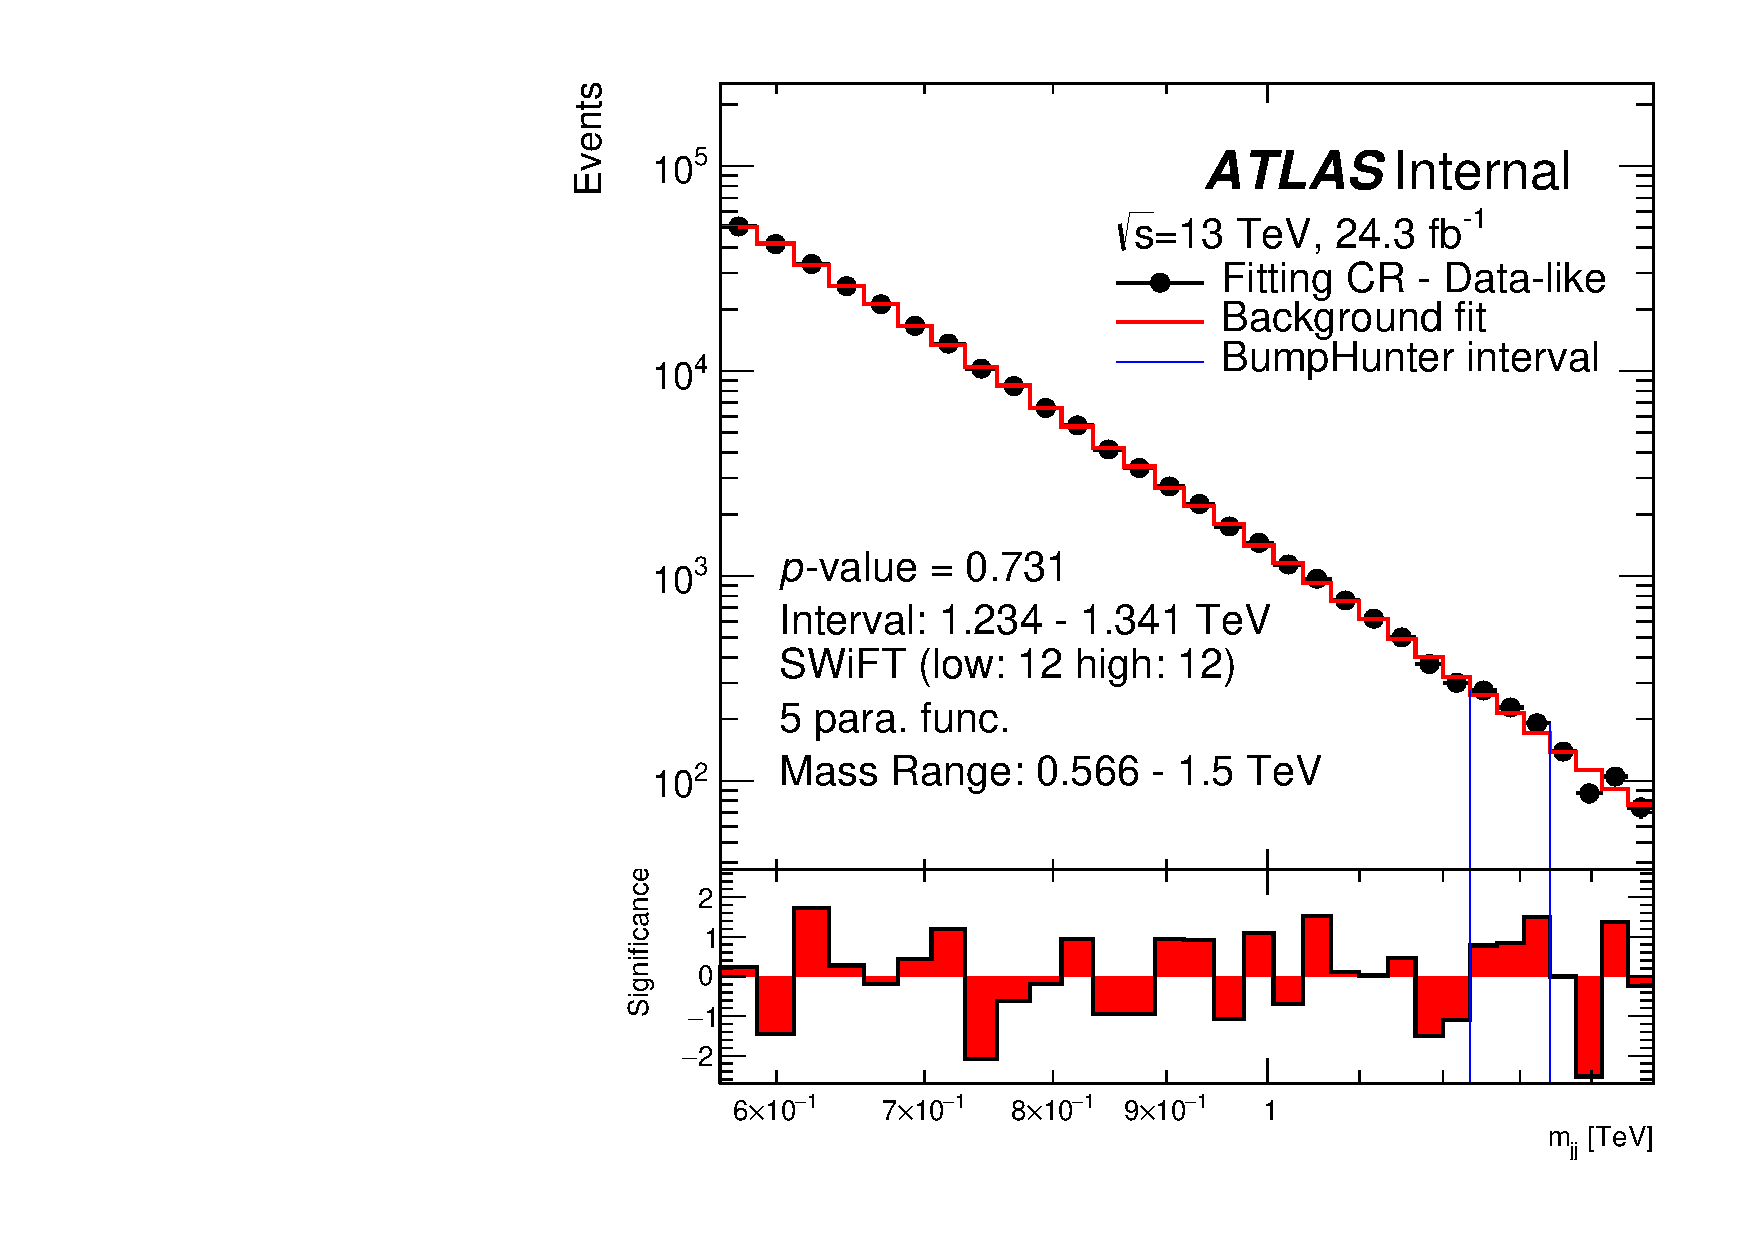
\includegraphics[width=0.48\linewidth, angle=0]{figs/Dibjet/LowMass/FitStudy_min566/bhFit_corrFitCR_dataLike_v13_5para_low12_high12.pdf}
}
\subcaptionbox{5 parameter fit, $wHW$ = 10} {
  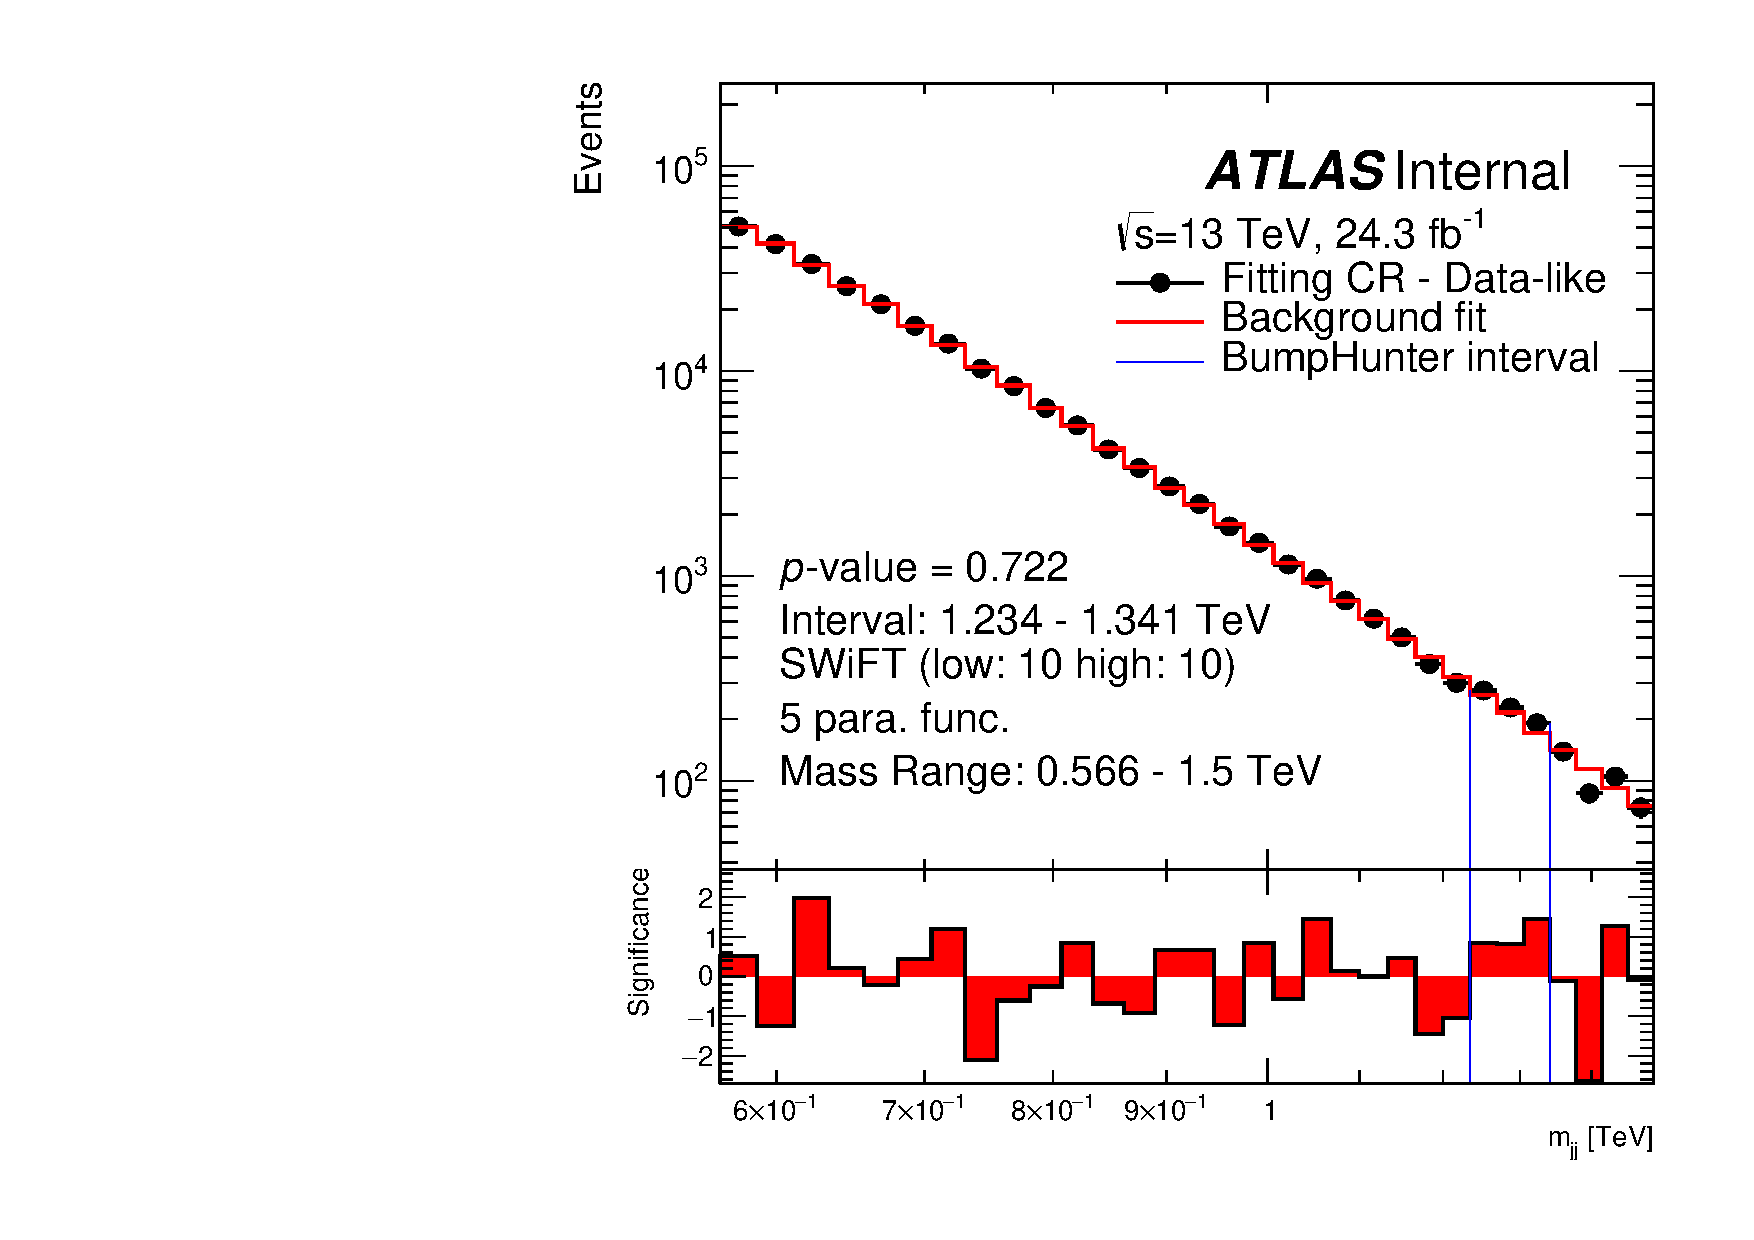
\includegraphics[width=0.48\linewidth, angle=0]{figs/Dibjet/LowMass/FitStudy_min566/bhFit_corrFitCR_dataLike_v13_5para_low10_high10.pdf}
}
\vspace{10pt}
\caption[Figure~\ref{fig:bhFit_lm_corrFitCR_dataLike} for all SWiFt configurations using the 5 parameter dijet fit function..]
{\label{fig:app-bhFit_lm_corrFitCR_dataLike_5para}
  Figure~\ref{fig:bhFit_lm_corrFitCR_dataLike} for all SWiFt configurations using the 5 parameter dijet fit function..
  The SWiFt search phase run on a data-like dijet mass spectrum
  from the fit control region for the \lm{} data-set.
  The SWiFt configurations considered use the 5 parameter dijet fit function for a window half-width ($wHW$) range of 10 to 16.
}
\end{figure}

\clearpage
\section{Figure~\ref{fig:bhFit_lm_corrFitCR_dataLike_inj_Zprimebb800_xsFactor1} for all SWiFt configurations.}
\vspace{5em}

\begin{figure}[!htb]
\captionsetup[subfigure]{aboveskip=0pt,justification=centering}
\centering
\subcaptionbox{4 parameter fit, $wHW$ = 16} {
  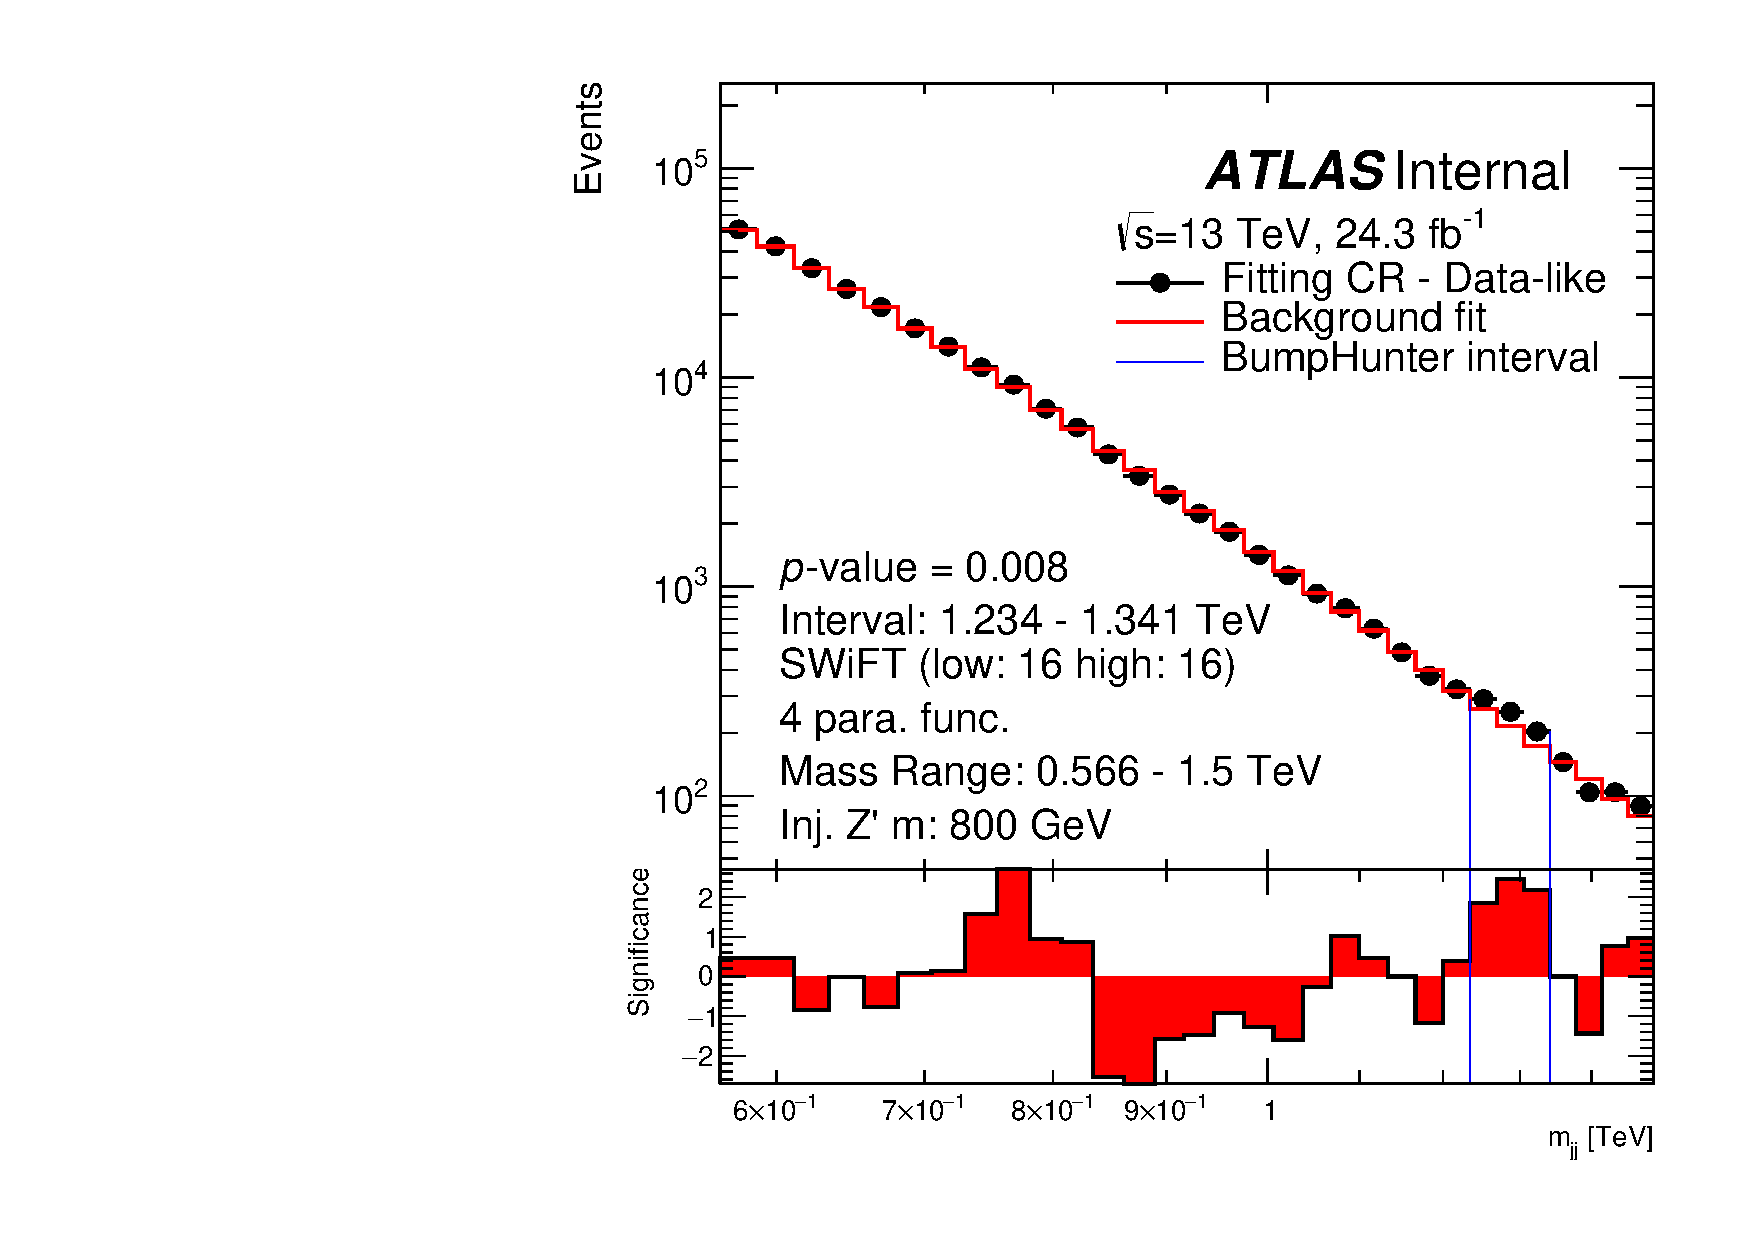
\includegraphics[width=0.48\linewidth, angle=0]{figs/Dibjet/LowMass/FitStudy_min566/bhFit_corrFitCR_dataLike_4para_low16_high16_inj_Zprimebb800_xsFactor1.pdf}
}
\subcaptionbox{4 parameter fit, $wHW$ = 14} {
  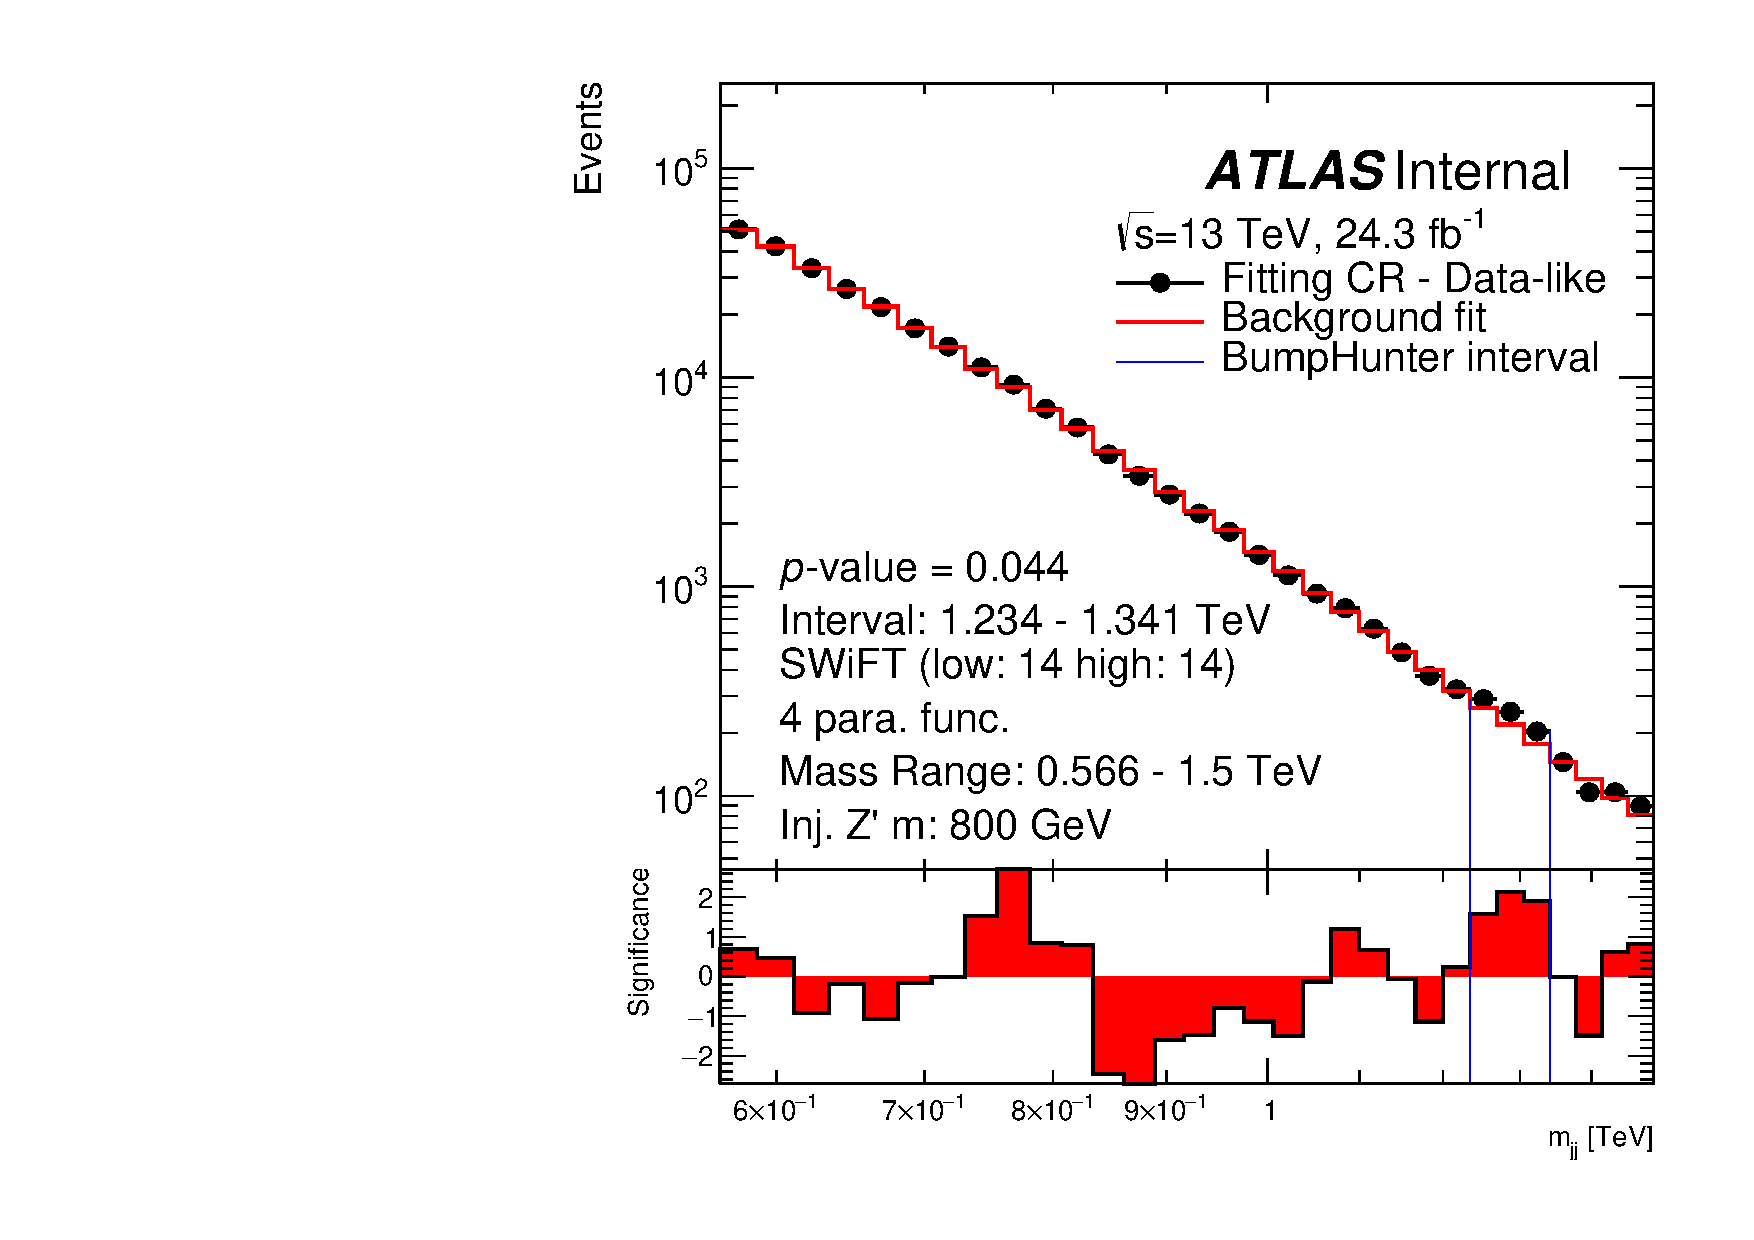
\includegraphics[width=0.48\linewidth, angle=0]{figs/Dibjet/LowMass/FitStudy_min566/bhFit_corrFitCR_dataLike_4para_low14_high14_inj_Zprimebb800_xsFactor1.pdf}
}
\subcaptionbox{4 parameter fit, $wHW$ = 12} {
  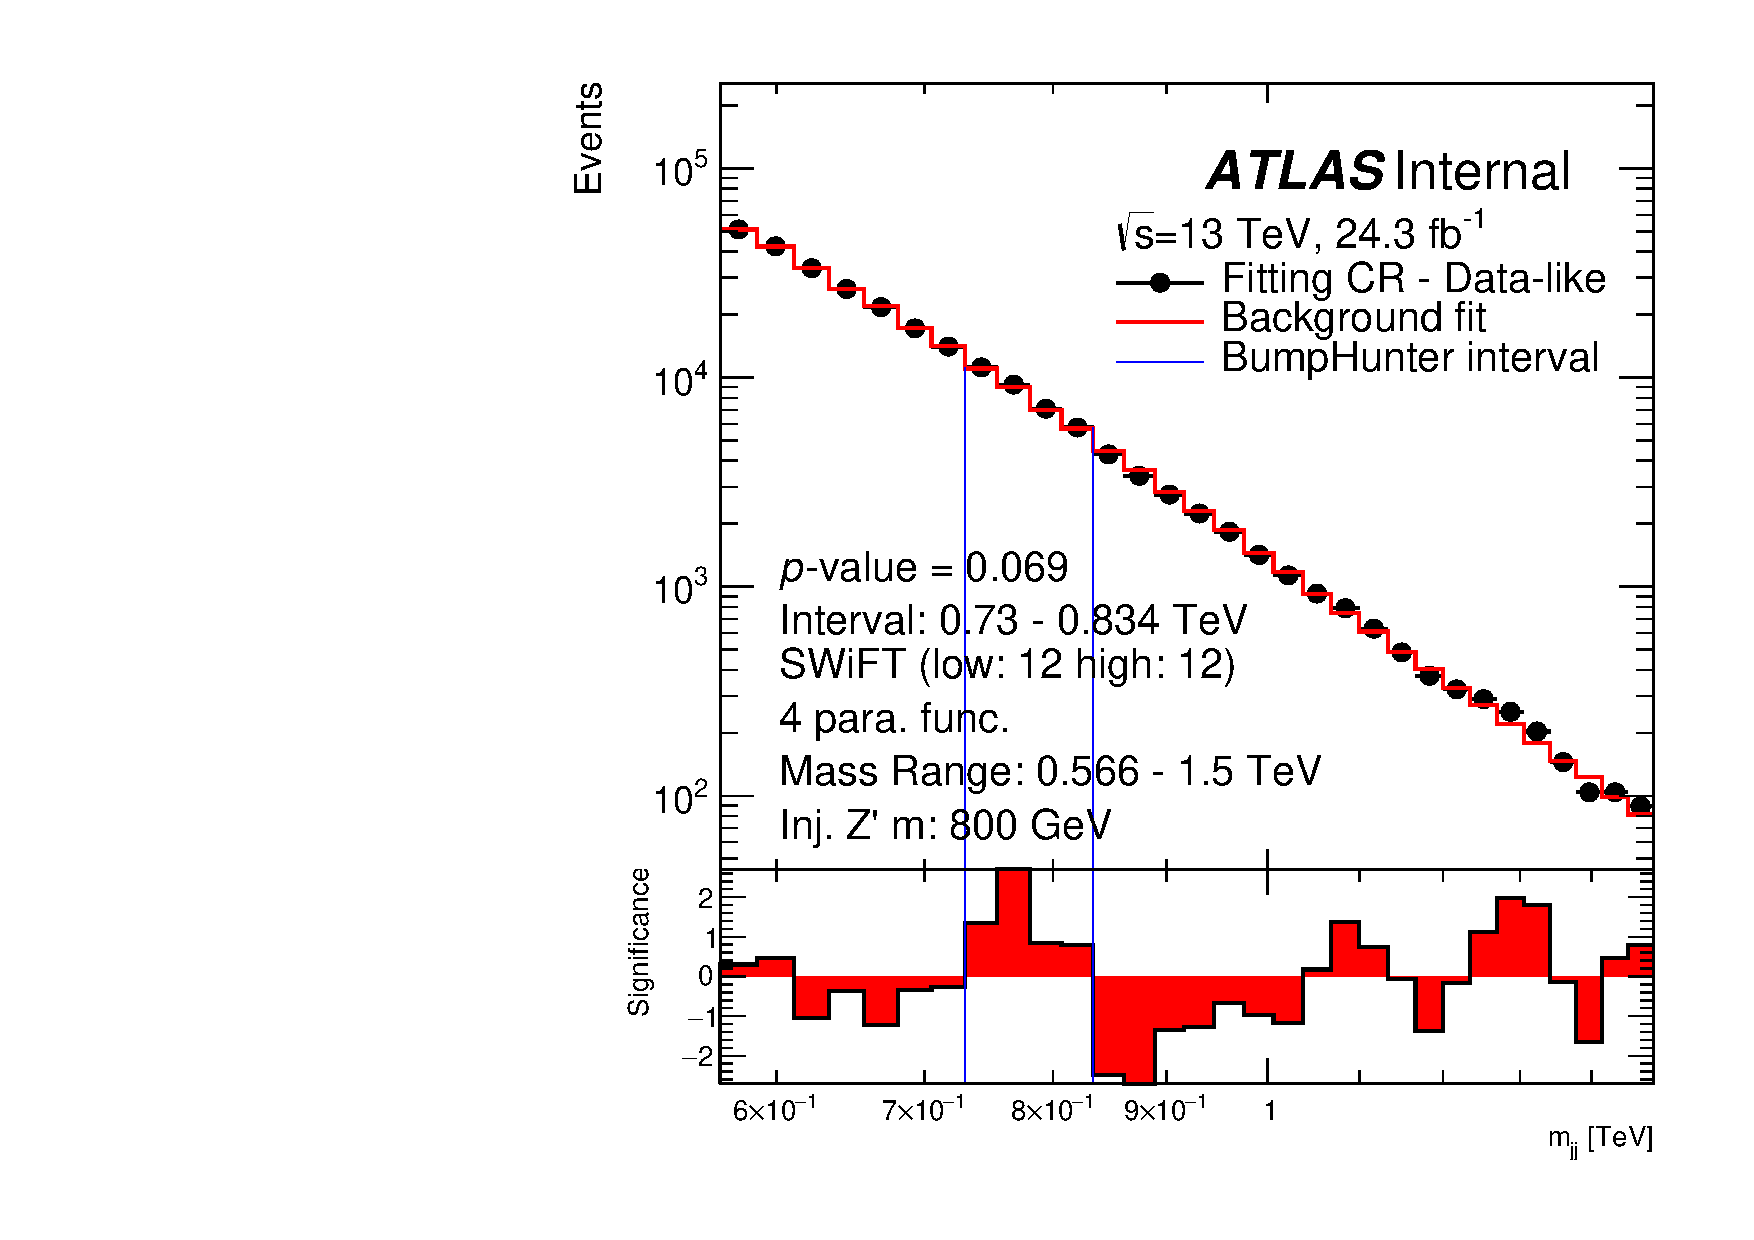
\includegraphics[width=0.48\linewidth, angle=0]{figs/Dibjet/LowMass/FitStudy_min566/bhFit_corrFitCR_dataLike_4para_low12_high12_inj_Zprimebb800_xsFactor1.pdf}
}
\subcaptionbox{4 parameter fit, $wHW$ = 10} {
  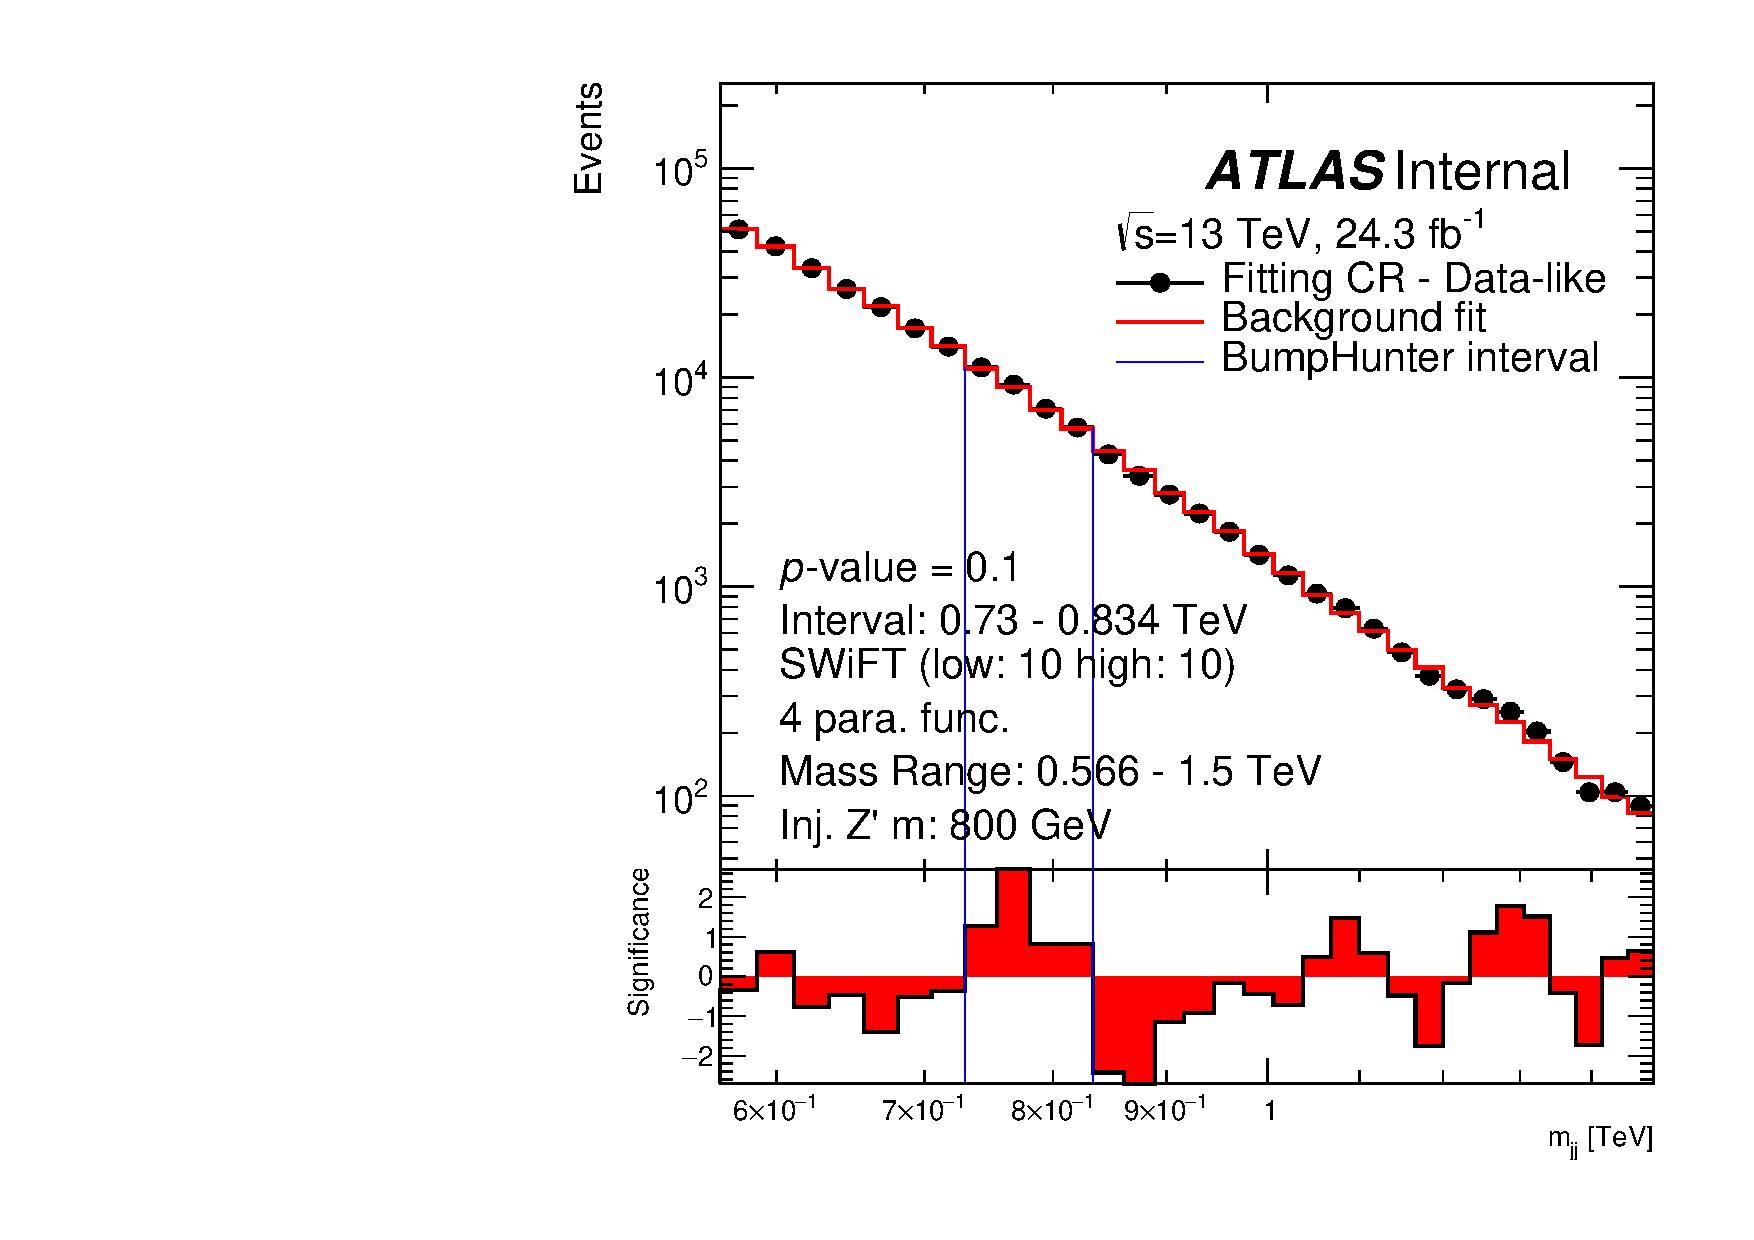
\includegraphics[width=0.48\linewidth, angle=0]{figs/Dibjet/LowMass/FitStudy_min566/bhFit_corrFitCR_dataLike_4para_low10_high10_inj_Zprimebb800_xsFactor1.pdf}
}
\caption[Figure~\ref{fig:bhFit_lm_corrFitCR_dataLike_inj_Zprimebb800_xsFactor1} for all SWiFt configurations using the 4 parameter dijet fit function..]
{\label{fig:app-bhFit_lm_corrFitCR_dataLike_inj_Zprimebb800_xsFactor1_4para}
Figure~\ref{fig:bhFit_lm_corrFitCR_dataLike_inj_Zprimebb800_xsFactor1} for all SWiFt configurations using the 4 parameter dijet fit function..    
  The SWiFt search phase run on a data-like dijet mass spectrum
  from the fit control region with a SSM $Z'$ of mass 800 GeV injected.
  The SWiFt configurations considered use the 4 parameter dijet fit function for a window half-width ($wHW$) range of 10 to 16.
}
\end{figure}
\begin{figure}[!htb]
\captionsetup[subfigure]{aboveskip=0pt,justification=centering}
\subcaptionbox{5 parameter fit, $wHW$ = 16} {
  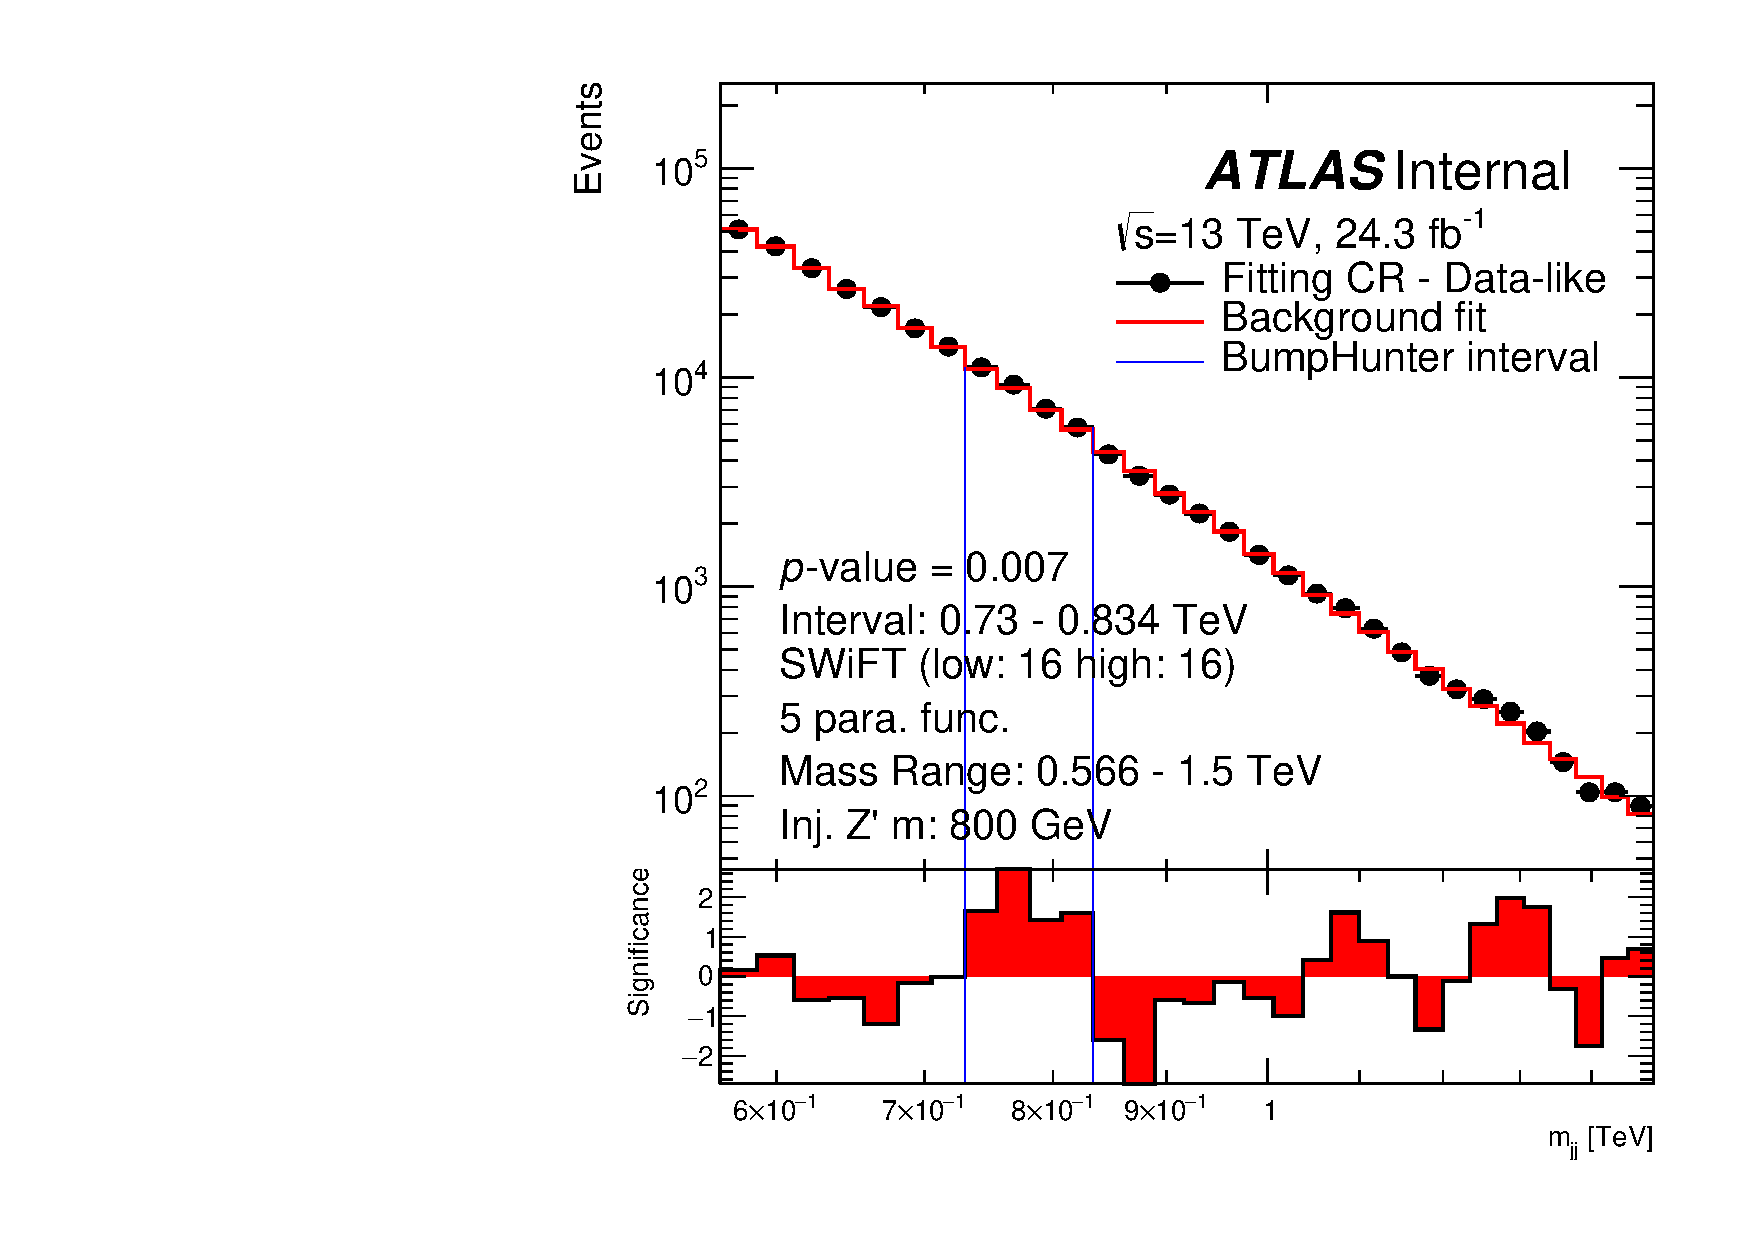
\includegraphics[width=0.48\linewidth, angle=0]{figs/Dibjet/LowMass/FitStudy_min566/bhFit_corrFitCR_dataLike_5para_low16_high16_inj_Zprimebb800_xsFactor1.pdf}
}
\subcaptionbox{5 parameter fit, $wHW$ = 14} {
  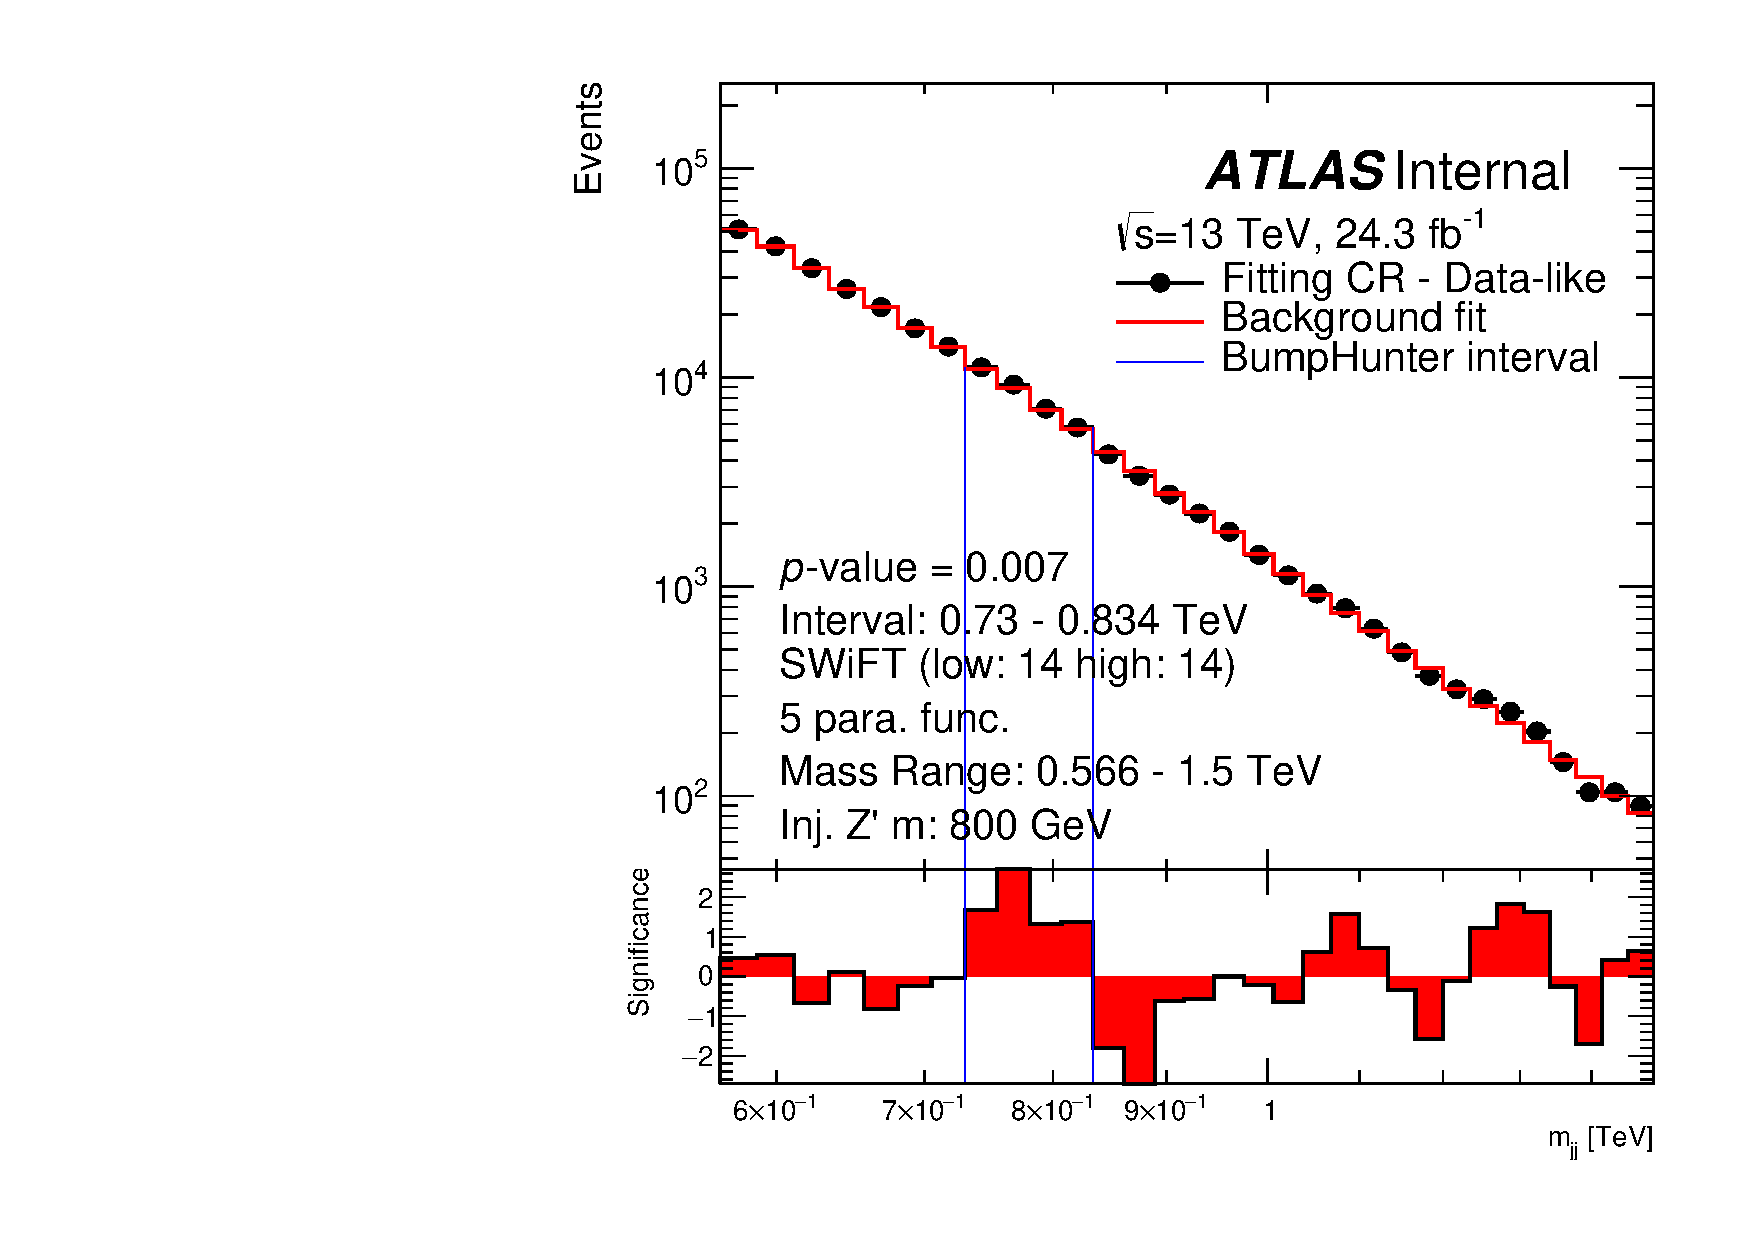
\includegraphics[width=0.48\linewidth, angle=0]{figs/Dibjet/LowMass/FitStudy_min566/bhFit_corrFitCR_dataLike_5para_low14_high14_inj_Zprimebb800_xsFactor1.pdf}
}
\subcaptionbox{5 parameter fit, $wHW$ = 12} {
  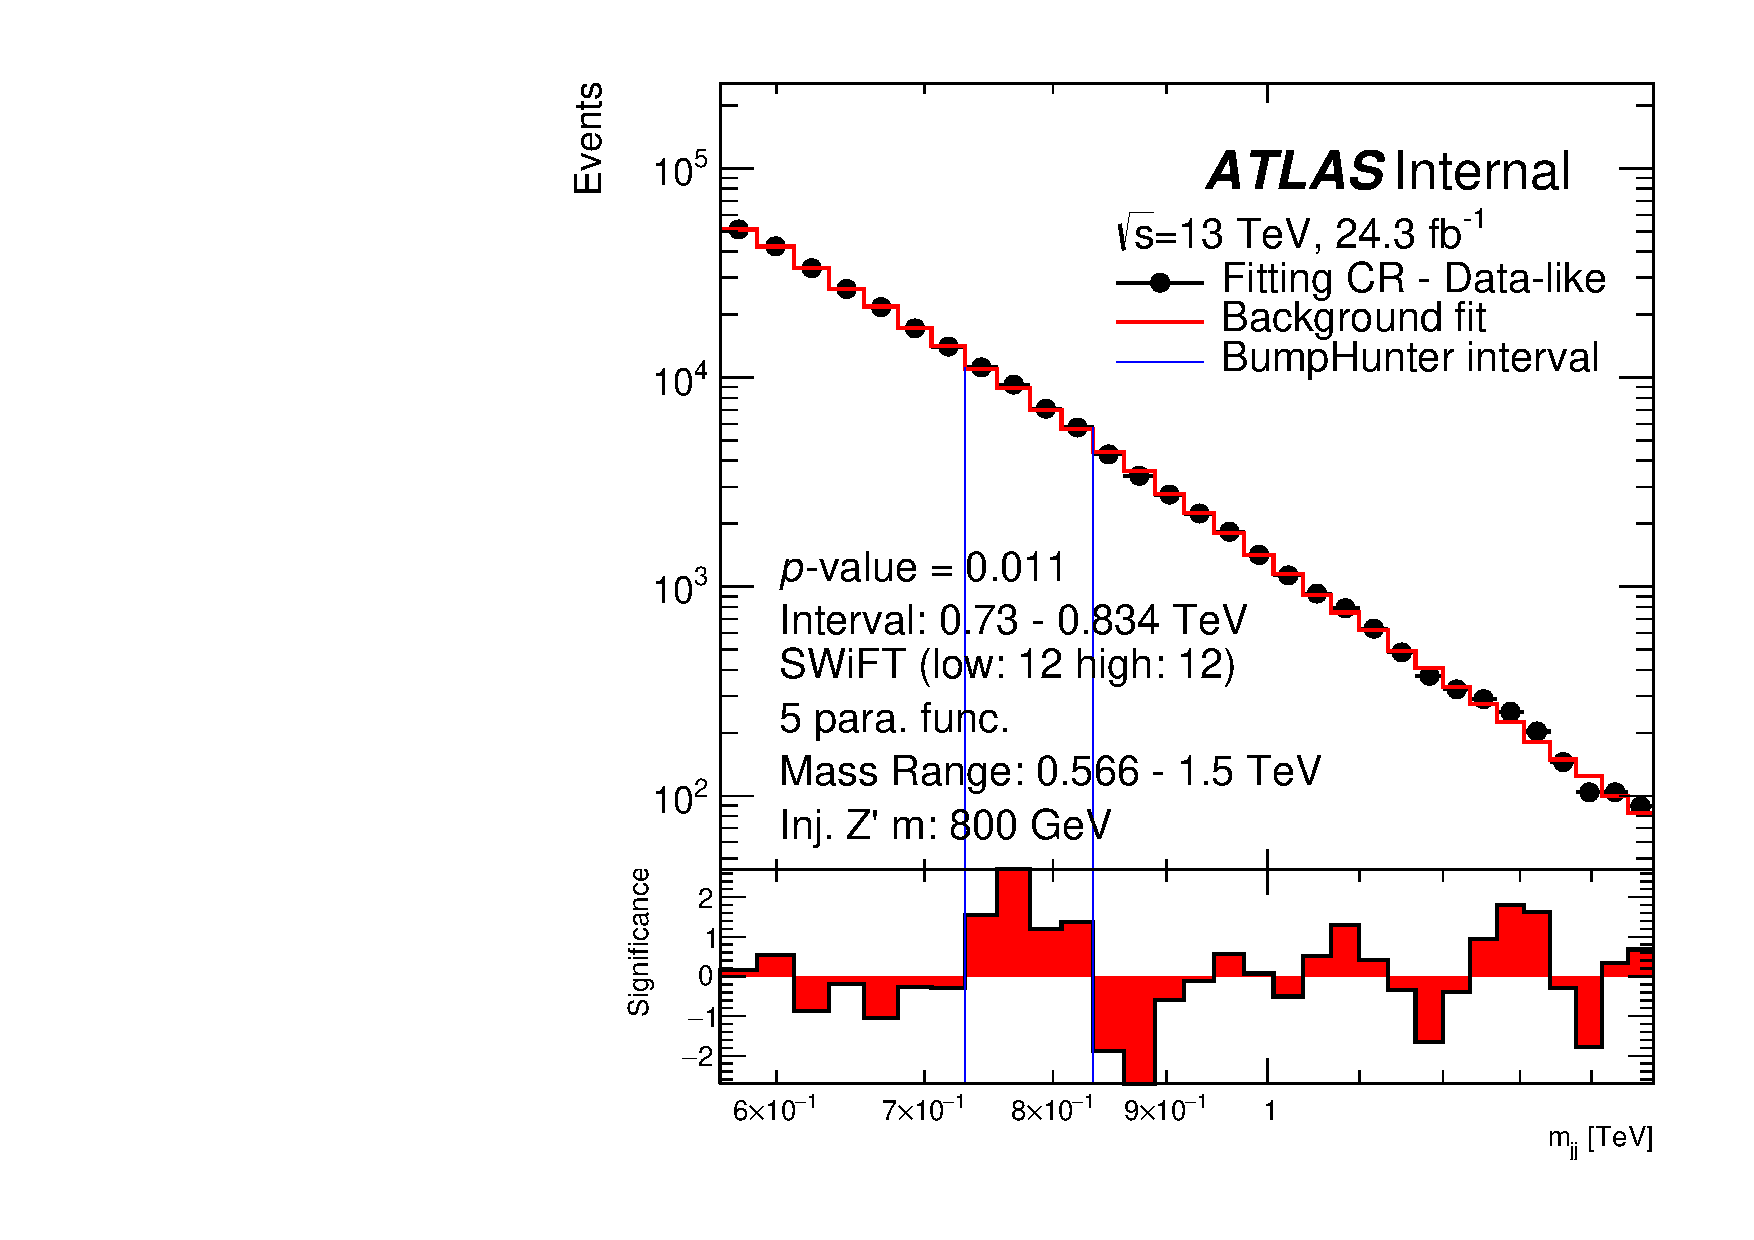
\includegraphics[width=0.48\linewidth, angle=0]{figs/Dibjet/LowMass/FitStudy_min566/bhFit_corrFitCR_dataLike_5para_low12_high12_inj_Zprimebb800_xsFactor1.pdf}
}
\subcaptionbox{5 parameter fit, $wHW$ = 10} {
  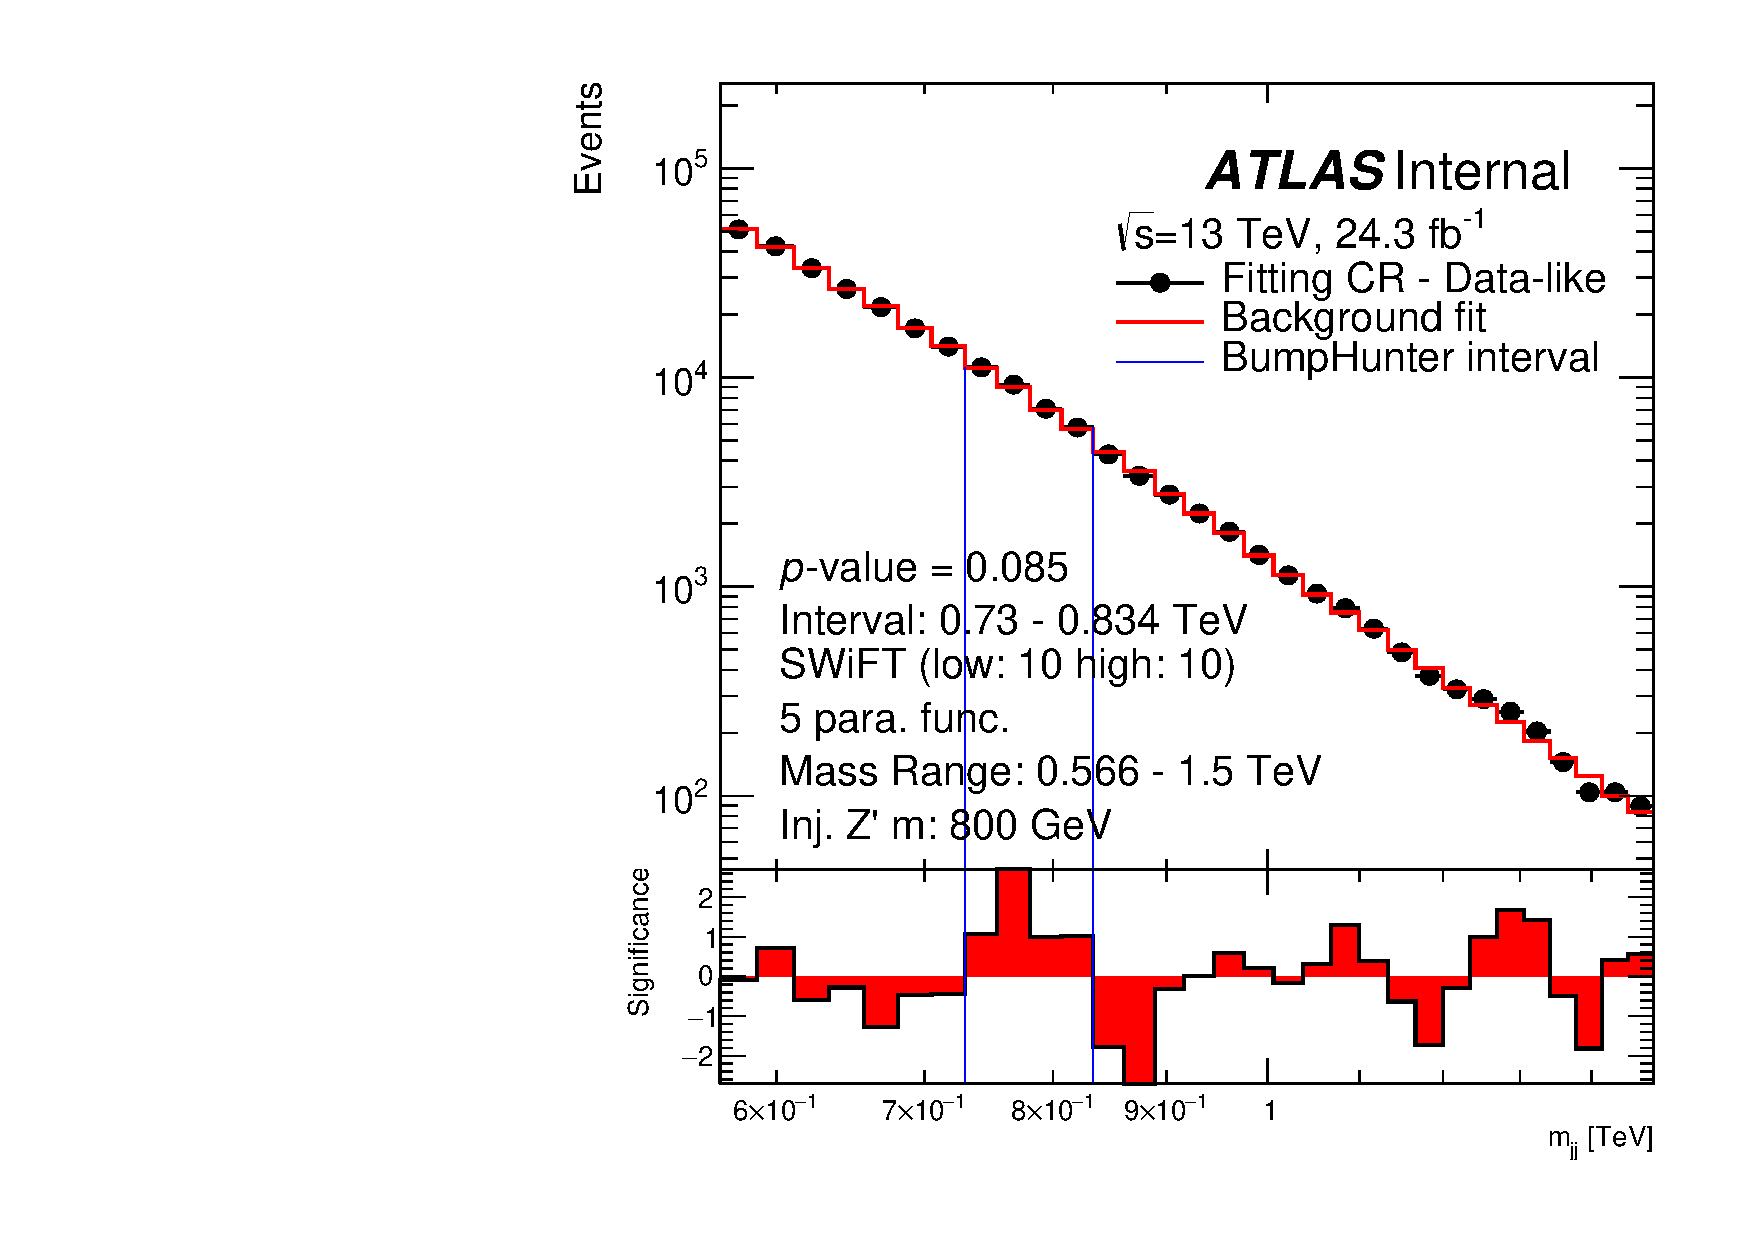
\includegraphics[width=0.48\linewidth, angle=0]{figs/Dibjet/LowMass/FitStudy_min566/bhFit_corrFitCR_dataLike_5para_low10_high10_inj_Zprimebb800_xsFactor1.pdf}
}
\vspace{10pt}
\caption[Figure~\ref{fig:bhFit_lm_corrFitCR_dataLike_inj_Zprimebb800_xsFactor1} for all SWiFt configurations using the 5 parameter dijet fit function.]
{\label{fig:app-bhFit_lm_corrFitCR_dataLike_inj_Zprimebb800_xsFactor1_5para}
Figure~\ref{fig:bhFit_lm_corrFitCR_dataLike_inj_Zprimebb800_xsFactor1} for all SWiFt configurations using the 5 parameter dijet fit function.    
  The SWiFt search phase run on a data-like dijet mass spectrum
  from the fit control region with a SSM $Z'$ of mass 800 GeV injected.
  The SWiFt configurations considered use the 5 parameter dijet fit function for a window half-width ($wHW$) range of 10 to 16.
}
\end{figure}

\addtocontents{toc}{\protect\setcounter{tocdepth}{2}}
